\documentclass{beamer}
%%%https://github.com/hdante/picat-lang/blob/master/doc/predfunc.tex
%\documentclass[10pt]{beamer} 
%\usetheme[pageofpages=of,% String used between the current page and the
          % total page count.
%          alternativetitlepage=true,% Use the fancy title page.
          %titlepagelogo=coca,% Logo for the first page.
%          titleline=true
%          ]{chameleon}
%\usetheme{Frankfurt}


\mode<presentation> {

% The Beamer class comes with a number of default slide themes
% which change the colors and layouts of slides. Below this is a list
% of all the themes, uncomment each in turn to see what they look like.

%\usetheme{default}
%\usetheme{AnnArbor}
%\usetheme{Antibes}
%\usetheme{Bergen}
%\usetheme{Berkeley}
\usetheme{Berlin}
%\usetheme{Boadilla}
%\usetheme{CambridgeUS}
%\usetheme{Copenhagen}
%\usetheme{Darmstadt}
%\usetheme{Dresden}
%\usetheme{Frankfurt}
%\usetheme{Goettingen}
%\usetheme{Hannover}
%\usetheme{Ilmenau}
%\usetheme{JuanLesPins}
%\usetheme{Luebeck}
%\usetheme{Madrid}
%\usetheme{Malmoe}
%\usetheme{Marburg}
%\usetheme{Montpellier}
%\usetheme{PaloAlto}
%\usetheme{Pittsburgh}
%\usetheme{Rochester}
%\usetheme{Singapore}
%\usetheme{Szeged}
%\usetheme{Warsaw}

% As well as themes, the Beamer class has a number of color themes
% for any slide theme. Uncomment each of these in turn to see how it
% changes the colors of your current slide theme.

%\usecolortheme{albatross}
%\usecolortheme{beaver}
%\usecolortheme{beetle}
%\usecolortheme{crane}
\usecolortheme{dolphin}
%\usecolortheme{dove}
%\usecolortheme{fly}
%\usecolortheme{lily}
%\usecolortheme{orchid}
%\usecolortheme{rose}
%\usecolortheme{seagull}
%\usecolortheme{seahorse}
%\usecolortheme{whale}
%\usecolortheme{wolverine}

%\setbeamertemplate{footline} % To remove the footer line in all slides uncomment this line
%\setbeamertemplate{footline}[page number] % To replace the footer line in all slides with a simple slide count uncomment this line

%\setbeamertemplate{navigation symbols}{} % To remove the navigation symbols from the bottom of all slides uncomment this line
}


%\usecolortheme{chameleon}

\usepackage{graphicx,hyperref,url}
\usepackage[utf8]{inputenc}
\usepackage[T1]{fontenc}
\usepackage[portuges,brazilian]{babel}
%%%\usepackage{wrapfig}
\usepackage{caption}
\usepackage{subfigure}
%\usepackage{subcaption}
\usepackage{latexsym}
\usepackage{amssymb, amsmath}
\usepackage{multicol}
\usepackage{pifont}%,bbding}%%,dingbat} %%% ver manual de simbolos
\usepackage[final]{listings}
\usepackage{comment}
\usepackage{array}
\usepackage{blindtext}
\usepackage{lipsum}

\setbeamertemplate{caption}[numbered]

\definecolor{azulclaro}{rgb}{0.9,0.9,0.9}
\definecolor{mygreen}{rgb}{0,0.6,0}
\definecolor{mygray}{rgb}{0.5,0.5,0.5}
\definecolor{mymauve}{rgb}{0.58,0,0.82}
\definecolor{darkgray}{rgb}{.4,.4,.4}
\definecolor{purple}{rgb}{0.65, 0.12, 0.82}

%\newcommand{\minizinc}{MiniZinc}

\newenvironment{CustomBlock}[3]{%
	\setbeamercolor{block body}{#2}
	\setbeamercolor{block title}{#3}
	\begin{block}{#1}}{\end{block}}

\lstset{ 
  %  label={pgm_ex01},
    backgroundcolor=\color{azulclaro}, 
    language=erlang, %%Miranda,%%Perl,%%%Python, %%Mercury,
    showstringspaces=false,
    basicstyle=\bf\scriptsize\ttfamily,
%%      basicstyle= \footnotesize %%% TESTAR
%%      keywordstyle=\bfseries\color{green!40!black},
    keywordstyle=\textbf{\color{mygreen}}, 
    otherkeywords={*, \%, array, constraint, solve, output,  show, "/\", satisfy, set, of, if, then, elseif, float, search},
%%  keywordstyle=\color{blue},       % keyword style
%%    commentstyle=\itshape\color{purple!40!black},
      commentstyle=\color{orange},    % comment style
      identifierstyle=\color{blue},
      stringstyle=\color{orange},
      stringstyle=\color{mymauve},
      numbers=left,  % where to put the line-numbers; possible values are (none, left, right)
      numbersep=5pt,   % how far the line-numbers are from the code
      numberstyle=\tiny\color{magenta},
      keepspaces=true      
    % %caption={LEGENDA no source PASCAL ficou OK},
}


\graphicspath{{/home/ccs/Dropbox/figs_genericas/}{figuras/}{/home/ccs/Dropbox/CCS/picat/}}
\DeclareGraphicsExtensions{.pdf,.png,.jpg}
%Global Background must be put in preamble
%\usebackgroundtemplate{\includegraphics[width=\paperwidth]{amarelinho.pdf}}
%%% \begin{frame}[allowframebreaks=0.8]

% The log drawn in the upper right corner.

%\logo{\centering
%\includegraphics[height=0.050\paperheight]{figuras/logo_SBPO_Peixe.png}
%%\hspace{9.6cm}
%\includegraphics[height=0.027\paperheight]{figuras/logo_udesc_horizontal.jpg}


%%%%%%%%%%%%%%%%%%%%%%%%%%%%%%%%%%%%%%%%%%%%%%%%%%%%%%%%%%%%%%%%%%%%%


\title[Picat]{\fontsize{20}{30}\selectfont \textcolor{black}{PICAT: Uma Linguagem de Programação Multiparadigma}}

\author[Claudio Cesar de Sá]{, Claudio Cesar de Sá, Miguel Alfredo Nunes, Jeferson L. R. Souza
\\\medskip 
	 {\small \url{miguel.nunes@edu.udesc.br}}\\
     {\small \url{jeferson.souza@udesc.br}}\\
     {\small \url{claudio.sa@udesc.br}}}

\institute[]{
    Departamento de Ci\^encia da Computa\c{c}\~ao -- DCC \\
    Centro de Ci\^encias e Tecnol\'ogias -- CCT\\
    Universidade do Estado de Santa Catarina -- UDESC}

%%%%%%%%%%%%%%%%%%%%%%%%%%%%%%%%%%%%%%%%%%%%%%%%%%%%%%%%%%%%%%%%%%%%%

\begin{document}
\begin{frame}
    \titlepage
\end{frame}

%%%%%%%%%%%%%%%%%%%%%%%%%%%%%%%%%%%%%%%%%%%%%%%%%%%%%%%%%%%%%%%%%%%%%
\begin{frame}[fragile]
  \frametitle{Contribuições}
  \begin{itemize}

    \item Alexandre Gonçalves;

    \item João Herique Faes Battisti;

    \item Paulo Victor de Aguiar;

    \item Rogério Eduardo da Silva;
    \item Hakan Kjellerstrand -- (\url{http://www.hakank.org/picat/})
    \item Neng-Fa Zhou -- (\url{http://www.picat-lang.org/})

    \item Outros anônimos que auxiliaram na produção deste documento;

  \end{itemize}

\end{frame}


%%%%%%%%%%%%%%%%%%%%%%%%%%%%%%%%%%%%%%%%%%%%%%%%%%%%%%%%%%%%%%%%%%%%%
%%%%%%%%%%%%%%%%%%%%%%%%%%%%%%%%%%%%%%%%%%%%%%%%%%%%%%%%%%%%%%
\section{Apresentação ao Curso de PICAT}

%%%The \pause command internally uses \onslide (see §9.1 of the beamer manual), so it does employ overlay specifications.


\begin{frame}[fragile]

  \frametitle{Apresentação ao Curso de PICAT -- I}
  \begin{itemize}
    \item O que é o PICAT?
    \pause
       \begin{itemize}
			\item Uma linguagem de programação de propósitos gerais
			\item Uma evolução do PROLOG (consagrada linguagem dos primórdios da IA)
			\item Tem elementos das linguagens Python, Prolog e Haskell
		\end{itemize}

    \item Uso e finalidades do PICAT:
    \pause
       \begin{itemize}
			\item Uso de programas gerais: de simples à complexos (uma reflexão)
			\item Provê suporte há vários \textit{solvers} na área de Pesquisa Operacional
			\item Área: IA, programação por restrições, programação inteira, planejamento,
			combinatória, etc
		\end{itemize}

   \end{itemize}

  \end{frame}
    
%\framebreak
\begin{frame}[fragile]
  \frametitle{Apresentação ao Curso de PICAT -- II}
  \begin{itemize}

    \item Este curso é dirigido a você?
  \pause
    \item Requisitos:
   \pause
		\begin{itemize}
			\item Conhecimento: noções de lógica matemática 
			(proposional e primeira-ordem), matemática elementar, 
			e alguma outra linguagem de programação

			\item Dedicação: depende de você
		\end{itemize}
		
  \pause
    \item Motivação:
   \pause
		\begin{itemize}
			\item Dependendo de sua dedicação, ao final você vai estar apto a resolver problemas
			computacionais de simples à difíceis

			\item Difícil: muitas linhas de código e muito conhecimento de algoritmos seriam
			necessários
			
			\item Com Picat, há sofisticados esquemas prontos para se construir programas.

		\end{itemize}

  \end{itemize}

\end{frame}


    
\begin{frame}[fragile]
  \frametitle{Apresentação ao Curso de PICAT -- III}
  \begin{itemize}
						
    \item Recursos computacionais:\\
    \pause 
    Binários disponíveis para Linux, Mac e Windows
     e Código fonte (em C) também disponível

    \item Comunidade e ações: \url{http://picat-lang.org}
    
    \pause
    \item Códigos e este material, sempre atualizados em: 

    \pause
    \begin{itemize}
      \item  Este PDF e seu texto original:  \url{http://github.com/claudiosa/Slides_Picat} (em código \LaTeX)
     \item   Os códigos fontes dos programas:  \url{http://github.com/claudiosa/CCS/picat}
    \end{itemize}

			\item Além do material aqui disponível em PDF, o mais importante  do curso
			 vai estar na interatividade
			da minha \textbf{apresentação oral}. 
			
    
  \end{itemize}

\end{frame}

    
\begin{frame}[fragile]
  \frametitle{Apresentação ao Curso de PICAT -- IV}
  \begin{itemize}

    \item Há alguns pontos do curso que estão repetidos: \textit{propositalmente}!\\
    \pause
    Reforça os erros que cometi um dia!

    \pause
    \item As aulas aqui apresentadas \textbf{não} serão regravadas!
        
    \pause 
    \item Contudo, o texto completo, incluindo os fontes dos programas: \textbf{SIM}\\
    Pois sempre há perguntas, melhoramentos, etc, que elucidam os pontos aqui abordados.
    
    \pause 
    \item Na parte teórica da definição do Picat, mantive os padrões 
    descritos no manual da linguagem (\url{http://picat-lang.org}).
    
  \end{itemize}

\end{frame}





    
\begin{frame}[fragile]
  \frametitle{Apresentação ao Curso de PICAT -- V}
  \begin{itemize}

    \item Além desta  apresentação do curso, você pode assistir uma
    parte deste curso em aulas que fiz para o Youtube, há alguns anos atrás:

    \pause
    \item Videoaula 01: Introdução ao PICAT\\
    \textbf{\url {https://www.youtube.com/watch?v=0DmTyFFQPK8}}

    \pause 
    \item Videoaula 02: Tipos de Dados do PICAT\\
    \textbf{\url {https://www.youtube.com/watch?v=7fPKPd0ZDnc}} 
    
    \item Estas videoaulas forem refeitas e  encontram-se com uma outra abordagem
    neste curso.
    
  \end{itemize}

\end{frame}




\begin{frame}[fragile]
  \frametitle{Apresentação ao Curso de PICAT -- VI}
  \begin{itemize}

						
    \item Assim, ao final deste curso terás uma sólida visão  de uma ferramenta
    computacional, utilizada em várias áreas tais como: modelagem matemática, IA,
    Pesquisa Operacional, etc

    \pause
    \item Ao final você vai conseguir resolver problemas com alguma complexidade e ler
    códigos de grandes programadores da área: Barták, Neng-Fa, Hakank, Dymichenko, etc    
    
    \pause
		\item Em resumo, este material é  um guia para o seu desenvolvimento,
		 com explicações nestas aulas, que funcionam como um \textit{atalho} de
		 horas de estudo sobre vários temas apresentados.
   
    \pause
    \item Tópicos   cobertos no curso: ver índice
  \end{itemize}

\end{frame}

%%%%%%%%%%%%%%%%%%%%%%%%%%%%%%%%%%%%%%%%%%%%%%%%%%%%%%%%%%%%%%%%%%%%%

 \begin{frame}[allowframebreaks,c]{Sumário}
  \tableofcontents
 \end{frame}
%%%%%%%%%%%%%%%%%%%%%%%%%%%%%%%%%%%%%%%%%%%%%%%%%%%%%%%%%%%%%%%%%%%%%

%%%%%%%%%%%%%%%%%%%%%%%%%%%%%%%%%%%%%%%%%%%%%%%%%%%%%%%%%%%%%%
\section{Introdução}
\begin{frame}

    \frametitle{Histórico}

    \begin{itemize}
      \item Criada em 2013 por Neng-Fa Zhou e Jonathan Fruhman

      \item Utiliza o B-Prolog como base de implementação, tendo
      a Lógica de Primeira-Ordem (LPO) como parte de seu mecanismo programação

\pause
      \item Uma evolução ao Prolog após seus mais de 40 anos de sucesso!

\pause
      \item Sua atual versão é a 2.x (\today).
\pause
      \item Código-aberto, segue as regras da FSF

    \end{itemize}
\end{frame}

%%%%%%%%%%%%%%%%%%%%%%%%%%%%%%%%%%%%%%%%%%%%%%%%%%%%%%%%%%%%%%%%%%%%%

\subsection{Estrutura da Linguagem}

\begin{frame}
	\frametitle{Conhecendo PICAT}
    
    \begin{itemize}
    
    	\item Picat é uma linguagem de programação simples de usar, poderosa e multi-uso
        
        \item Alguma de suas características 
         são associadas com linguagens lógicas, como Prolog, B-Prolog, Goedel, etc
        
        \pause
        \item Picat é uma linguagem essencialmente multiparadigma,
        abrangendo partes de vários paradigmas de programação: declarativo (lógico e funcional) e     imperativo
        
        %\item Esta combinação de características declarativas e imperativas permite
        %o desenvolvimento de softwares mais produtivos, mas que ainda possam ser altamente 
        %otimizados para tarefas específicas, ou softwares mais simples para tarefas mais mundanas;
        
    \end{itemize}
    
\end{frame}

%%%%%%%%%%%%%%%%%%%%%%%%%%%%%%%%%%%%%%%%%%%%%%%%%%%%%%%%%%%%%%%%%%%%%

\begin{frame}[fragile]
    \frametitle{O que é ser Multiparadigma ?}

    \begin{itemize}
    
    \item Paradigma: um conjunto de características baseado em alguma abordagem teórica 
    
    \pause
      \item Picat é uma linguagem multiparadigma pois abrange os seguintes paradigmas:
    
      \begin{itemize}
      	\item[--] Lógico
      	\item[--] Funcional
      	\item[--] Procedural
      \end{itemize}
      
     \pause
      \item Em resumo,  \textit{uma boa mistura} de: Haskell (Funcional) , Prolog (Lógica) e 
      Python (Procedural e Funcional).
      
    \end{itemize}
      

\end{frame}

%%%%%%%%%%%%%%%%%%%%%%%%%%%%%%%%%%%%%%%%%%%%%%%%%%%%%%%%%%%%%%%%%%%%%
\subsubsection{Paradigmas}
\begin{frame}[fragile]
	\frametitle{Paradigma Lógico}
    
    \begin{itemize}
    
    	\item Uma linguagem lógica é uma onde o programa é expresso como um conjunto
        de predicados lógicos, escritos por \textit{fatos} e \textit{regras}
    
    \pause
    	\item Regras são escritas em formas de cláusulas, as quais são interpretadas como
        implicações lógicas.\\ 
        Dependem das premissas serem verdadeiras para esta ser verdadeira.
        

    \pause
    	\item Fatos são cláusulas sem premissas, verdades absolutas.

        
        \pause
        \item Este   paradigma é a  \textbf{base} do Picat
    \end{itemize}

\end{frame}

%%%%%%%%%%%%%%%%%%%%%%%%%%%%%%%%%%%%%%%%%%%%%%%%%%%%%%%%%%%%%%%%%%%%%

\begin{frame}[fragile]
	\frametitle{Paradigma Funcional}
    
    \begin{itemize}
    
    
    	\item Uma linguagem funcional é uma onde os elementos do programa podem ser avaliados e 
        tratados como funções matemáticas.
        
        \pause
         \item Um dos principais motivos em usar linguagens funcionais é a previsibilidade
         e facilidade no entendimento do estado atual do programa.
         
         \pause
         \item Este fato de uma  sintaxe simples, torna o Picat  intuitivo e legível na
         funcionalidade de seus códigos.
         
    \end{itemize}
    
    
\end{frame}

%%%%%%%%%%%%%%%%%%%%%%%%%%%%%%%%%%%%%%%%%%%%%%%%%%%%%%%%%%%%%%%%%%%%%

\begin{frame}[fragile]
	\frametitle{Paradigma Procedural}
    
    \begin{itemize}
    
    	\item Uma linguagem procedural é uma que pode ser subdividida em \textit{procedimentos},
        também chamados de rotinas, subrotinas ou funções
        
        \pause
        \item Em linguagens procedurais há um procedimento principal (em geral é chamado de 
        \textit{Main}) que controla o uso e a chamada de outros procedimentos. Em Picat há
        tal hierarquia.
        
        \pause
        \item Em Picat, cada premissa é tratada como um procedimento, que é resolvido por meio
        de métodos de inferência lógica.
       
    \end{itemize}
    
\framebreak
    
    \begin{figure}
    	\begin{columns}
    		\column{.6\linewidth}
	         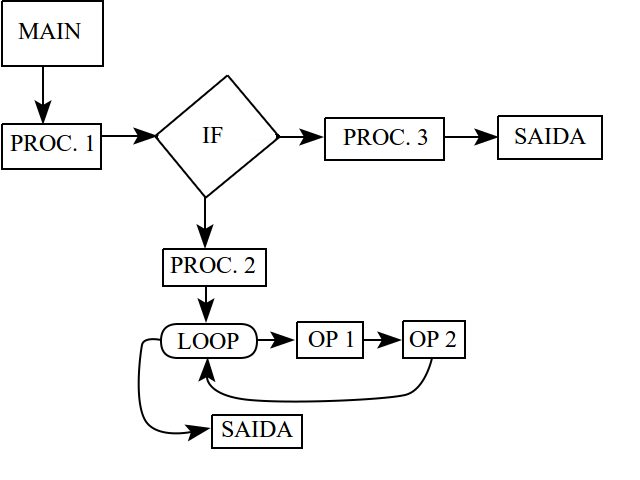
\includegraphics[width=.8\textwidth] {figures/Paradigma_Procedural.png}
             \column{.4\linewidth}
             \caption{Fluxograma representando a estrutura de um programa Procedural}
	         \label{Fluxograma Procedural}
		\end{columns}
	\end{figure}
    
\end{frame}

%%%%%%%%%%%%%%%%%%%%%%%%%%%%%%%%%%%%%%%%%%%%%%%%%%%%%%%%%%%%%%%%%%%%%

\begin{frame}[fragile]
    \frametitle{Algumas Características:}

    \begin{itemize}
    
    \pause 
      \item Sintaxe elegante e simples, facilitando a leitura e entendimento do código
      
          \pause 
      \item Velocidade de execução em um ambiente \textit{interpretado} (há
      uma \textit{máquina
      virtual} como Python, Java e alguns Prologs)
      
          \pause 
      \item Disponibilidade em vários sistemas operacionais e arquiteturas
      
      \pause 
      \item Análogo a Python, podem ser feitas \textit{queries}
      ou \textit{consultas} ao terminal de Picat.

      \pause 
      \item Há várias bibliotecas da própria linguagem, e diversas ferramentas
      externas permitindo o incremento do poder do Picat.
      
    \end{itemize}
\end{frame}

%%%%%%%%%%%%%%%%%%%%%%%%%%%%%%%%%%%%%%%%%%%%%%%%%%%%%%%%%%%%%%%%%%%%%


\begin{frame}	 [fragile]

   \frametitle{Acrônimo de \textbf{P.I.C.A.T.}}
  
  
  \begin{block}{}
  		\begin{description}

 \item [\textbf{P}:] \textit{Pattern-matching}:  Utiliza o conceito de \textit{casamento de 
padrões} entre objetos, bem como os conceitos da \textit{unificação} da LPO

\item [\textbf{I}:] \textit{Intuitive}: Oferece estruturas de decisão, atribuição e laços de
repetição, etc. Análogo há outras linguagens de programação mais populares

\item [\textbf{C}:] \textit{Constraints}: Suporta a programação por restrições (PR) para 	
problemas combinatórios

 \item [\textbf{A}:] \textit{Actors}: Suporte as chamadas a eventos, chamada via \textit{atores}

\item [\textbf{T}:] \textit{Tabling}: Implementa a técnica de \textit{memoization} com 
soluções imediatas para problemas de Programação Dinâmica (PD).

  \end{description}	
 \end{block}
  
\end{frame}

%%%%%%%%%%%%%%%%%%%%%%%%%%%%%%%%%%%%%%%%%%%%%%%%%%%%%%%%%%%%%%%%%%%%%

\begin{frame}[fragile]
  \frametitle{Instalação do PICAT}

  \begin{itemize}
   	\item Baixar a versão desejada de:\\ 
    \hspace{8mm} \url{http://picat-lang.org/download.html}

     \pause    
   	\item Descompactar. Em geral em: \textbf{/usr/local/Picat/} ou \textbf{/opt/Picat/}  no Linux e IOS

     \pause    
    \item  Criar um link simbólico (Linux) ou atalhos (Windows):\\ 
    
   	\hspace{8mm}\texttt{ln -s /usr/local/Picat/picat   \hspace{3mm}   /usr/bin/picat}

    \pause    
    \item Se quiser adicionar (opcional) uma variável de ambiente:\\
          \hspace{8mm} \texttt{PICATPATH=/usr/local/Picat/}\\
          \hspace{8mm} \texttt{export PICATPATH}

     \pause
    \item Ou ainda, adicione o caminho: \texttt{PATH=\$PATH:/usr/local/Picat}

     \pause
   	\item Finalmente, tenha um editor de texto apropriado.\\
    \hspace{8mm} Sugestão: \textit{Geany}, \textit{Sublime} ou \textit{VS Code}.

  \pause
   	\item Editor on-line mantido pelo Alexandre: \url{http://retina.inf.ufsc.br/picat.html}
     
    \pause
    \item Se não tiver \textit{plugin} para Picat, escolha a sintaxe da linguagem \textit{Erlang}.
    
  \end{itemize}

\end{frame}

%%%%%%%%%%%%%%%%%%%%%%%%%%%%%%%%%%%%%%%%%%%%%%%%%%%%%%%%%%%%%%%%%%%%%

\subsubsection{Usando Picat}

\begin{frame}[fragile]
  \frametitle{Usando Picat}
  	\begin{itemize}
    
    % \item Picat é uma linguagem  disponível em qualquer arquitetura de 
    % processamento. 
      
    %\pause
    %\item Qualquer emergência, o ambiente completo de execução do Picat pode ser reconstruído a partir da linguagem C padrão
      
   
      \item Os seus arquivos fontes utilizam a extensão \textbf{.pi}. Exemplo: \texttt{programa.pi}
      \item Há dois modos principais de utilização do Picat: 
      
      \begin{itemize}
      	\item[--] Modo interativo, onde seu código é digitado e compilado diretamente na linha de 
        comando;
      	\item[--] \textit{Modo console} onde o console só é utilizado para compilar seus programas.
      \end{itemize}
      
      \pause
      \item Códigos executáveis 100\% \textbf{stand-alone}: ainda não!
      \item Neste quesito, estamos em igualdade com Java, Prolog e Python
     
    \end{itemize}
\end{frame}





\begin{frame}[fragile]
\frametitle{Exemplo -- \textit{Alô Mundo!}}

Acompanhar as explicações do código de:\\
\url{https://github.com/claudiosa/CCS/blob/master/picat/alo_mundo.pi}

\begin{verbatim}
main => msg_01  , 
        msg_02 .
        
msg_01 =>  printf("  ALO MUNDO!!! ").
msg_02 =>  printf("\n  FIM \n").
\end{verbatim}

\end{frame}


\begin{frame}[fragile]
\frametitle{Execução na Console Linux ou Windows}

\begin{verbatim}
$ picat alo_mundo.pi 
  ALO MUNDO!!! 
  FIM 
$ 
\end{verbatim}

\pause
\textcolor{red}{Análogo ao desenvolvimento com Python!}

\end{frame}


\begin{frame}[fragile]
\frametitle{Execução no Ambiente do Interpretador}

\begin{footnotesize}
\begin{verbatim}
$ picat
Picat 2.0, (C) picat-lang.org, 2013-2016.
Type 'help' for help.
Picat> cl(álo_mundo.pi').
Compiling:: alo_mundo.pi
alo_mundo.pi compiled in 0 milliseconds
loading...

yes

Picat> main 
  ALO MUNDO!!! 
  FIM 

yes

Picat> msg_02

  FIM 

yes

Picat> 
\end{verbatim}

\end{footnotesize}
\end{frame}


\begin{frame}[fragile]
\frametitle{Ambiente do Interpretador -- Uso do \texttt{getline}}

\begin{itemize}
  \item Inicialmente, aqui o código foi carregado com o comando `\texttt{cl}' (digite \texttt{help} na console), o qual \textbf{compila} o seu código e \textbf{carrega} em um código intermediário pronto
  para ser executado e testado
  
  \pause
  \item Neste ambiente interpretado há comandos básicos de teclado (mouse não funciona aqui)
  do programa \texttt{getline} do Linux. Os mais importantes são:
  \pause
  \begin{itemize}
    \item  \textbf{Crtl-a}: move o cursor para o início da linha
        \item  \textbf{Crtl-e}: move o cursor para o final da linha (\textit{end})
        \item  \textbf{Crtl-f}: 	move o cursor de uma posição a frente (forward)
         \item  \textbf{Crtl-b}: 	move o cursor de uma posição para trás (backward)
         \item  \textbf{Crtl-d}: 	exclui o carácter sob  o cursor (a 2a. vez -- sai do ambiente)
        \item  \textbf{Crtl-u}: 	exclui a linha inteira
        \item As flechas ... repetem os últimos comandos
  \end{itemize}
  
\end{itemize}

\end{frame}



\begin{frame}[fragile]
\frametitle{Ambiente do Interpretador -- Uso}

\begin{itemize}
  \item Use um editor externo de sua preferência. Por exemplo:
   \texttt{geany} com plugin do Picat

    \pause
  \item Mantenha duas janelas de terminais abertas
    \begin{itemize}
    \item Uma para o ambiente interpretado
    \item Outra para usá-lo diretamente: \texttt{\$console\$ picat seu\_programa.pi}
  \end{itemize}
  
    \pause
  \item Os dois modos são importantes de se trabalhar simultaneamente
  
  \pause
  \item Em dúvidas, digite: \texttt{Picat> help .}
    
\end{itemize}

\end{frame}












\begin{frame}[fragile]
\frametitle{Reflexões}

\begin{itemize}


  \item O conteúdo desta parte do curso pode ser complementado
  com a   \textbf{Videoaula 01: Introdução ao PICAT}, disponível no Youtube:\\
    \textbf{\url {https://www.youtube.com/watch?v=0DmTyFFQPK8}}

      \pause
      \item Para próxima seção esteja com o Picat instalado em seu 
      computador para um melhor aproveitamento.
   % \pause
  %\item 
\end{itemize}

\end{frame}

%%%%%%%%%%%%%%%%%%%%%%%%%%%%%%%%%%%%%%%%%%%%%%%%%%%%%%%%%%%%%%%%%%%%%

\section{Tipos de Dados e Variáveis}

\begin{frame}[fragile]
%[fragile, allowframebreaks=0.9]
 \frametitle{Tipos de Dados e Variáveis -- Introdução -- I}


\begin{itemize}

\item Em projetos de linguagens de programação há dois tipos 
verificação do tipo de dados: \underline{\textbf{estática}} e \underline{\textbf{dinâmica}}

  
  \pause 
  \item A verificação de tipos dados   \underline{estática} 
   em \textit{tempo de compilação}.
  
    \pause 
  \item Enquanto a \underline{dinâmica} em \textit{tempo de execução}.
  
  \pause 
  \item Linguagens fortemente tipadas, tais como C, Java e Pascal, 
  exigem que o tipo do dado (conteudo) seja do mesmo tipo da variável 
  ao qual este valor será atribuído. 
  Tudo isto é pré-definido durante a fase da \textit{compilação}.
  
  
\end{itemize}
\end{frame}


\begin{frame}[fragile]
%[fragile, allowframebreaks=0.9]
 \frametitle{Tipos de Dados e Variáveis -- Introdução -- II}
\begin{itemize}

  \item Nas linguagens interpretadas, com uma máquina virtual, 
  esta definição é feita durante a \textit{execução} do
  programa
  
  \pause 
  \item Prós e contras para o que é melhor, a discussão fica de lado neste momento
  
  \pause 
  \item Picat até o momento tem a tipagem \textbf{dinâmica}
  
\end{itemize}


\end{frame}


%%%%%%%%%%%%%%%%%%%%%%%%%%%%%%%%%%%%%%%%%%%%%%%%%%%%%%%%%%%%%%%%%%%%%

\subsection{Tipos de Dados}


\begin{frame}
	\frametitle{Tipos de Dados}
	

	\begin{figure}[!ht]
		\centering
		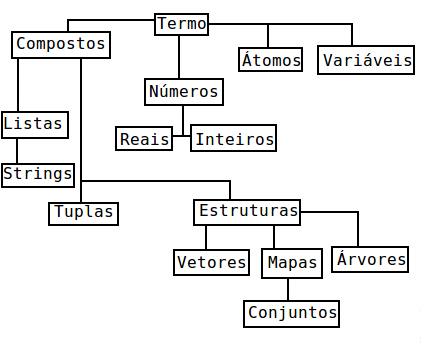
\includegraphics[width = .725\linewidth]{figures/tipos_dados_picat__traduzido3.png}
		\caption{Hierarquia dos Tipos de Dados}
		\label{fig:TiposDados}
	\end{figure}
	% imagem estilo da imagem de paradigmas
\end{frame}

%%%%%%%%%%%%%%%%%%%%%%%%%%%%%%%%%%%%%%%%%%%%%%%%%%%%%%%%%%%%%%%%%%%%%

\begin{frame}
%[fragile, allowframebreaks=0.9]
	\frametitle{Termos}

\begin{itemize}
	  \item Em Picat, variáveis e valores são \textit{genericamente} chamados de \textit{termos}
	
	  \pause 
	  \item Os valores são subdivididos em duas categorias, números e valores 
	compostos
	
		  \item Os números, por suas vez, podem ser inteiros ou reais, e valores compostos
	podem ser listas e estruturas
	
	%\pause 
	%\item Resumindo, em Picat tudo é \textit{termo}
	
	\end{itemize}	
\end{frame}

%%%%%%%%%%%%%%%%%%%%%%%%%%%%%%%%%%%%%%%%%%%%%%%%%%%%%%%%%%%%%%%%%%%%%

\begin{frame}[fragile]
	\frametitle{Átomos}
	
	\begin{itemize}
	  \item Átomos são constantes simbólicas, podendo ser delimitados ou não, por 
	aspas simples.
	
	\item Carácteres são representados por átomos de comprimento $1$.
	
	 	\item Átomos não delimitados por aspas simples, \underline{\textbf{nunca}} começam com uma letra maiúscula, nem número ou \textit{underscore}.

	\end{itemize} 

	  \pause 
	\begin{exampleblock}{Exemplos}
		\begin{verbatim}
		x   x_1   '_'   '\\'   'a\'b\n'   '_ab'   '$%'
		\end{verbatim}
	\end{exampleblock}
	
\end{frame}

%%%%%%%%%%%%%%%%%%%%%%%%%%%%%%%%%%%%%%%%%%%%%%%%%%%%%%%%%%%%%%%%%%%%%

\begin{frame}[fragile, allowframebreaks=0.9]

	\frametitle{Números}
	
	Números se dividem em:
	
	\begin{itemize}
		
		\item \textbf{Inteiro:} Inteiros podem ser representados por números binários, octais,
		decimais ou hexadecimais.
		% Dígitos em um número podem ser separados por um 
		% \textbf{underscore}, porém essa separação é ignorada pelo compilador.
		
	\end{itemize}
	
	\begin{exampleblock}{Exemplos}
		\begin{tabbing}
			aa \= aaa \= aaa \= aaa \= aaa \= aaa \= aaa \kill
			\> \texttt{12\_345} \> \> \> 12345 em notação decimal, usando \_ como separador \\
			\> \texttt{0b100} \> \> \> 4 em notação binária  \\
			\> \texttt{0o73} \> \> \>  59 em notação octal \\
			\> \texttt{0xf7} \> \> \>  247 em notação hexadecimal  
		\end{tabbing}
	\end{exampleblock}

\textcolor{red}{O \textbf{underscore} é ignorado pelo compilador e o interpretador.}

\framebreak
	
	\begin{itemize}
		
		\item \textbf{Real:} Números reais são compostos por um parte inteira, um ponto,
		 seguido por uma fração decimal, ou um expoente.
		
		\item Se existe uma parte inteira em um número real então ela deve ser seguida por uma
		fração ou um expoente. Isso é necessário para distinguir um número real de um número inteiro.
	\end{itemize}
	
	\begin{exampleblock}{Exemplos}
		\begin{verbatim}
		12.345   0.123   12-e10   0.12E10
		\end{verbatim}
	\end{exampleblock}
	
\end{frame}

%%%%%%%%%%%%%%%%%%%%%%%%%%%%%%%%%%%%%%%%%%%%%%%%%%%%%%%%%%%%%%%%%%%%%

\begin{frame}
	\frametitle{Compostos}
	\begin{itemize}
	  \item 	Termos compostos podem conter mais de um valor ao mesmo tempo. 
	  
	  \pause
    \item   Termos compostos são 
	acessados pela notação de índice, começando a partir de $1$ e indo até $N$, onde $N$
	 é o tamanho deste termo.

	  \pause
    \item 	Se dividem em \underline{Listas} e \underline{Estruturas}.
	
    
	\end{itemize}
	
	
	
\end{frame}

%%%%%%%%%%%%%%%%%%%%%%%%%%%%%%%%%%%%%%%%%%%%%%%%%%%%%%%%%%%%%%%%%%%%%

\begin{frame}
	\frametitle{Listas}
	
	Listas são agrupamentos de valores quaisquer sem ordem e sem tamanho pré-definido. Seu tamanho não é 
	armazenado na memória, sendo necessário recalcular sempre que necessário seu uso. Listas são 
	encapsuladas por colchetes.
	
	\begin{exampleblock}{Exemplos}
		[1,2,3,4,5] \: [a,b,32,1.5,aaac] \: ["string",14,22]
	\end{exampleblock}

\textcolor{red}{Há uma seção dedicada a esta poderosa  estrutura de dados!}
	
\end{frame}

%%%%%%%%%%%%%%%%%%%%%%%%%%%%%%%%%%%%%%%%%%%%%%%%%%%%%%%%%%%%%%%%%%%%%

\begin{frame}
	\frametitle{\textit{Strings} -- Lista de Carácteres}
	
	\textit{Strings} são listas especiais que contém somente carácteres. \textit{Strings} podem ser inicializadas como uma 
	sequência de carácteres encapsulados por aspas duplas, ou como uma sequência de carácteres dentro 
	colchetes separados por vírgulas.
	
	\begin{exampleblock}{Exemplos}
		"Hello" \: "World!" \: "\textbackslash n" \: [o,l,a,"\:",m,u,n,d,o] 
	\end{exampleblock}
	
\end{frame}

%%%%%%%%%%%%%%%%%%%%%%%%%%%%%%%%%%%%%%%%%%%%%%%%%%%%%%%%%%%%%%%%%%%%%

\begin{frame}
	\frametitle{Tuplas}
	\begin{itemize}
	  \item 	Tuplas é um conjunto de termos não-ordenados, podendo ser acessados por notação de índice assim como	listas.
	  
	  \item  Tuplas são estáticas, ou seja, os termos contidos em uma tupla não podem ser alterados, assim como	não podem ser adicionados ou removidos termos de tuplas.
	  
	\item   Tuplas são encapsuladas por parênteses e seus termos são separados por vírgulas.

	\end{itemize}
	
	\begin{exampleblock}{Exemplos}
		(1,2,3,4,5) \: (a,b,32,1.5,aaac) \: ("string",14,22)
	\end{exampleblock}
	
	\textcolor{red}{Em geral, usamos as tuplas dentro de listas.}
\end{frame}

%%%%%%%%%%%%%%%%%%%%%%%%%%%%%%%%%%%%%%%%%%%%%%%%%%%%%%%%%%%%%%%%%%%%%

\begin{frame}
	\frametitle{Estruturas (\textit{Functores})}
	
	Estruturas são termos especiais que podem ser definidos pelo usuário. Estruturas tomam a seguinte 
	forma: 
	
	\begin{displaymath}
	\texttt{{\$}s($t_1,\ldots,t_n$)}
	\end{displaymath}
	
	Onde \textit{`s'} é um átomo que denomina a estrutura, cada 
	\textit{`$t_i$'} é um de seus termos, e \textit{`n'} é a aridade ou tamanho da estrutura.
	
	\begin{exampleblock}{Exemplo}
		\$ponto(1,2) \: \$pessoa(jose, "123.456.789.00", "1.234.567")
	\end{exampleblock}
	
	\pause
	\textbf{\textcolor{red}{Temos 4 outras estruturas  que não usam o símbolo \$, são elas:}}
	
\end{frame}

%%%%%%%%%%%%%%%%%%%%%%%%%%%%%%%%%%%%%%%%%%%%%%%%%%%%%%%%%%%%%%%%%%%%%

\begin{frame}
	\frametitle{Vetores} [fragile, allowframebreaks=0.9]
	
	Vetores ou \textit{arrays} são estruturas especiais do tipo:
	\begin{center}
		 \texttt{\{$t_1$,$\ldots$,$t_{n}$\}}
		\end{center}
	
	\begin{itemize}
	 \pause
	   \item Vetor é um conjunto ordenado de tamanho $n$, delimitado por \texttt{'\{\}'}.
	   \item 	Vetores tem comportamentos análogo às listas, tanto é que quase todas as funções de listas
	são sobrecarregadas para vetores. 
	
		   \item A diferença entre vetores e listas é que vetores tem um tamanho  constante.
		   \item Vetores são muito práticos quando se manipula matrizes na entrada
		   
	 \end{itemize} 

	
	\begin{exampleblock}{Exemplos}
		\{1,2,3,4,5\} \: \{a,b,32,1.5,aaac\} \: \{"string",14,22\}
	\end{exampleblock}
	
\end{frame}

%%%%%%%%%%%%%%%%%%%%%%%%%%%%%%%%%%%%%%%%%%%%%%%%%%%%%%%%%%%%%%%%%%%%%

\begin{frame}
	\frametitle{Mapas, Conjuntos e \textit{Heaps}}
	
	\begin{itemize}
		\item \textbf{Mapas} são estruturas especiais que são conjuntos de relações do tipo \texttt{chave-valor}.
		
		\item \textbf{Conjuntos} são sub-tipos de mapas onde todos as chaves estão relacionadas com o átomo 
		\texttt{not\_a\_value}.
		
		\item \textit{Heaps} são árvores binárias completas representadas como vetores.
		Árvores podem ser do tipo \textit{máximo}, onde o maior valor está na raiz, ou \textit{mínimo}, 
		onde o menor valor esta na raiz.
	\end{itemize}
	
\end{frame}

%%%%%%%%%%%%%%%%%%%%%%%%%%%%%%%%%%%%%%%%%%%%%%%%%%%%%%%%%%%%%%%%%%%%%

\subsection{Variáveis}

\begin{frame}[allowframebreaks=0.90]
	\frametitle{Variáveis}
	
	\begin{itemize}
		
		\item Picat é uma linguagem de \underline{Tipagem Dinâmica}, ou seja, o tipo de uma variável 
		é validado durante a execução do programa
		
		
		\item Isto é, quando uma variável é criada, seu tipo não é instanciado
		
		\item Variáveis são análogas as da matemática, são símbolos que \textit{seguram} ou 
		representam um valor
		
		\item Ao contrário de variáveis em linguagens imperativas, variáveis em Picat não são
		endereços simbólicos de locais na memória
		
		\item Uma variável é dita \textit{livre} (\textit{free}) se não contém nenhum valor, e dita
		\textit{instanciada} (\textit{bound}) se ela contém um valor
		
		\item Uma vez que uma variável é instanciada, ela permanece com este valor na 
		execução atual
		
		\item Por isso, diz-se que variáveis em Picat são de \textit{atribuição única}
		
		\framebreak
		\item O nome de variáveis devem sempre ser iniciado com letras \textbf{\underline{maisculas}}
		ou  com o caráctere \textbf{\textit{underscore (\_)}}, porém;
		
		\begin{itemize}
			
			\item Variáveis cujo nome é unicamente um caractere \textbf{\_} são chamadas de 
			\textit{variáveis anônimas}.
			
			\item As 			\textit{variáveis anônimas} podem receber qualquer  valor
			 não os guardam  durante a execução do programa;
			
			\item Num mesmo programa, podem existir diversas variáveis anônimas, instanciadas durante a execução do mesmo
			
		\end{itemize}
		
	\end{itemize}
	
\end{frame}

%%%%%%%%%%%%%%%%%%%%%%%%%%%%%%%%%%%%%%%%%%%%%%%%%%%%%%%%%%%%%%%%%%%%%

\subsection{Unificação e Atribuição}

\begin{frame}
	\frametitle{Unficação e Atribuição}
	Há dois modos de definir valores a variáveis, a \underline{unificação}, que usa o operador 
	\textbf{=}, e a \underline{atribuição}, que usa o operador \textbf{:=}
\end{frame}

%%%%%%%%%%%%%%%%%%%%%%%%%%%%%%%%%%%%%%%%%%%%%%%%%%%%%%%%%%%%%%%%%%%%%

\begin{frame}[fragile]
	\frametitle{Unificação}
	% definição:
	% casamento de padrão
	% unificação (Algoritmo da Unificação)
	% montar uma figura talvez
	\begin{itemize}
		
		\item A \textbf{\underline{Unificação}} é uma operação que instância uma variável a um termo ou 
		padrão, substituindo toda a ocorrência dessa variável pelo valor a qual ela foi instanciada até que
		haja uma situação onde esta instanciação falhe, nesse momento a variável será reinstanciada e
		esse processo se repete.
		
		\item Caso ocorra uma instância que não falhe nenhuma situação a variável é unificada à este termo
		ou padrão.
		
		\item Uma instanciação é indefinida até que se encontre um valor que possa ser unificada a uma
		variável.
        
        \item Termos são ditos unificáveis se são idênticos ou podem ser tornados idênticos instanciado 
        variáveis nos termos.
		
	\end{itemize}
	
\end{frame}

%%%%%%%%%%%%%%%%%%%%%%%%%%%%%%%%%%%%%%%%%%%%%%%%%%%%%%%%%%%%%%%%%%%%%

\begin{frame}[fragile]
	
	\begin{exampleblock}{Exemplo}
		
		\begin{verbatim}
		Picat> X = 1
		X = 1
		Picat> $f(a,b) = $f(a,b)
		yes
		Picat> [H|T] = [a,b,c]
		H = a
		T = [b,c]
		Picat> $f(X,b) = $f(a,Y)
		X = a
		Y = b
		Picat> bind_vars({X,Y,Z},a)
		Picat> X = $f(X)
		\end{verbatim}
		
		A última consulta demonstra um caso do problema de ocorrência, onde o compilador de Picat não
		verifica se um termo ocorre dentro de um padrão. Isso cria um termo cíclico que não pode ser
		acessado. % Algo muito ruim
		
	\end{exampleblock}
	
\end{frame}

%%%%%%%%%%%%%%%%%%%%%%%%%%%%%%%%%%%%%%%%%%%%%%%%%%%%%%%%%%%%%%%%%%%%%
\begin{frame}[fragile]
	\frametitle{Atribuição}
	
	\begin{itemize}
		
		\item A \textbf{\underline{Atribuição}} é uma operação cujo intuito é simular a atribuição em
		linguagens imperativas, permitindo que variáveis sejam re-atribuídas valores durante a execução
		do programa
		
		\item Para isso, durante a compilação do programa, toda vez que a operação de unificação é 	
		encontrada, uma nova variável temporária será criada que irá substituir a variável que seria
		atribuída.
		
	\end{itemize}
	
\end{frame}

%%%%%%%%%%%%%%%%%%%%%%%%%%%%%%%%%%%%%%%%%%%%%%%%%%%%%%%%%%%%%%%%%%%%%

\begin{frame}[fragile]
	
	\begin{exampleblock}{Exemplo}
		
		\begin{verbatim}
		test => X = 0, X := X + 1,  X := X + 2, write(X).
		\end{verbatim}
		Neste exemplo $X$ é unificado a $0$, então, o compilador tenta unificar $X$ a $X+1$, porém $X$ já 
		foi unificado a um valor, portanto outras operações devem ser feitas para que esta atribuição seja
		possível.\\
		
		Nesse caso, o compilador irá criar uma variável temporária, $X1$ por exemplo, e à ela irá unir
		$X+1$, depois toda vez que $X$ for encontrado no programa o compilador irá substitui-lo por $X1$.\\
		
		O mesmo ocorre na atribuição $X1 := X1 + 2$, neste caso uma outra variável temporária será criada,
		$X2$ por exemplo, e o processo será repetido.\\
		
		Portanto, estas atribuições sucessivas são compiladas como:
		
		\begin{verbatim}
		test => X = 0, X1 = X + 1, X2 = X1 + 2, write(X2).
		\end{verbatim} 
		
	\end{exampleblock}
	
\end{frame}

%%%%%%%%%%%%%%%%%%%%%%%%%%%%%%%%%%%%%%%%%%%%%%%%%%%%%%%%%%%%%%%%%%%%%

\begin{frame}[fragile]
	
	\begin{exampleblock}{Exemplos de Variáveis Válidas}
		
		\begin{center}
			\begin{tabular}{|c|c|c|}\hline
				X1 & \textbf{\_} & \_ab \\ \hline
				X & A & Variavel \\ \hline
				\_invalido & \_correto & \_aa \\ \hline
			\end{tabular}
		\end{center}
		
		Relembrando, um nome de variável é válido se começa com letra maiúscula ou \_
		
	\end{exampleblock}
	
\end{frame}

%%%%%%%%%%%%%%%%%%%%%%%%%%%%%%%%%%%%%%%%%%%%%%%%%%%%%%%%%%%%%%%%%%%%%

\begin{frame}[fragile]
	
	\begin{exampleblock}{Exemplos de Variáveis Inválidas}
		
		\begin{center}
			\begin{tabular}{|c|c|c|}\hline
				\verb!1_Var! & variavel & valida\\ \hline
				$23$ & \verb!"correto! & \verb!'termo!\\ \hline
				\verb+!numero+ & \verb!$valor! & \verb!#comum!\\ \hline
			\end{tabular}
		\end{center}
		
		Relembrando, um nome de variável é inválido se começa com números ou símbolos que não sejam 
		\_ ou letra minúscula
		
	\end{exampleblock}
	
\end{frame}

%%%%%%%%%%%%%%%%%%%%%%%%%%%%%%%%%%%%%%%%%%%%%%%%%%%%%%%%%%%%%%%%%%%%%

\subsection{Tabela de Operadores} 
\begin{frame}[fragile]
	
	\begin{table}
		\caption{\label{Operadores Aritméticos}Operadores Aritméticos em Ordem de Precedência}
		\begin{center}
			\begin{tabular}{ c|c } \hline
				\texttt{$X$ ** $Y$}  &  Potenciação \\ \hline 
				\texttt{$X$ * $Y$} &    Multiplicação \\ \hline 
				\texttt{$X$ / $Y$} &    Divisão, resulta em um real \\ \hline 
				\texttt{$X$ // $Y$} &    Divisão de Inteiros, resulta em um inteiro \\ \hline 
				\texttt{$X$ mod $Y$} &   Resto da Divisão\\ \hline
				\texttt{$X$ + $Y$} & Adição \\ \hline 
				\texttt{$X$ - $Y$} &   Subtração \\ \hline 
				{\tt $Inicio$ \verb!..! $Passo$ \verb!..! $Fim$} & Uma série (lista) de números com um passo\\ 
				\hline 
				{\tt $Inicio$ \verb!..! $Fim$}  &   Uma série (lista) de números com passo 1 \\ \hline
			\end{tabular}
		\end{center}
	\end{table}
	
\end{frame}

%%%%%%%%%%%%%%%%%%%%%%%%%%%%%%%%%%%%%%%%%%%%%%%%%%%%%%%%%%%%%%%%%%%%%

\begin{frame}[fragile]
	\begin{table}
		\caption{Tabela de Operadores Completa em Ordem de Precedência}
		\begin{center}
			\begin{tabular}{ c|c } \hline
				Operadores Aritméticos & Ver Tabela \ref{Operadores Aritméticos}\\ \hline
				\verb-++-  & Concatenação de Listas/Vetores \\ \hline 
				\verb+=+  \verb+:=+  & Unificação e Atribuição\\ \hline
				\verb+==+ \verb+=:=+ & Equivalência e Equivalência Numérica\\ \hline
				\verb+!=+ \verb+!==+ & Não Unificável e Diferença\\ \hline
				\verb+<+  \verb+=<+ \verb+<=+ & Menor que\\ \hline
				\verb+>+  \verb+>=+ & Maior que\\ \hline
				\verb+in+ & Contido em\\ \hline
				\verb+not+ & Negação Lógica \\ \hline 
				\verb+,+  $\&\&$ & Conjunção Lógica \\ \hline 
				\verb+;+  $|$$|$ & Disjunção Lógica \\ \hline 
			\end{tabular}
		\end{center}
	\end{table}
\end{frame}

%%%%%%%%%%%%%%%%%%%%%%%%%%%%%%%%%%%%%%%%%%%%%%%%%%%%%%%%%%%%%%%%%%%%%

\subsubsection{Operadores Especiais}

\begin{frame}[fragile,c]
    \frametitle{Operadores Especiais \textrm{\MakeUppercase{\romannumeral 1}}}
    
    \begin{block}{Operadores de Termos Não Compostos}

		\begin{enumerate}
    
            \item \textbf{Equivalência}(\verb+==+): Compara se dois termos são iguais.\\No caso de termos
            compostos, eles são ditos equivalentes se todos os termos contidos em si são equivalentes. O 
            compilador considera termos de tipos diferentes como totalmente diferentes, portanto a comparação 
            $1.0 == 1$ seria avaliada como falsa, mesmo que os valores sejam iguais. Nesses casos, usa-se a 
            \emph{Equivalência Numérica}.

            \item \textbf{Equivalência Numérica}(\verb+=:=+): Compara se dois números são o mesmo valor.
            Não deve ser usada com termos que não são números.

            \item \textbf{Diferença}(\verb+!==+): Compara se dois termos são diferentes.\\Mesmo que a negação da 
            equivalência.

            \item \textbf{Não Unificável}(\verb+!=+): Verifica se dois termos não são unificáveis. Termos são 
            ditos unificáveis se são idênticos ou podem ser tornados idênticos instanciando variáveis destes 
            termos.
    	\end{enumerate}
    \end{block}
    
\end{frame}

%%%%%%%%%%%%%%%%%%%%%%%%%%%%%%%%%%%%%%%%%%%%%%%%%%%%%%%%%%%%%%%%%%%%%

\begin{frame}

	\begin{exampleblock}{Exemplos}
    	
    	\begin{enumerate}
    	
          \item $a\:$==$\:a$, \: $[1,2,3]\:$==$\:[1,2,3]$, \: $Var1\:$==$\:Var2$\\
          \pause
          $yes$, $yes$, Depende dos Valores (padrão $no$)
          \medskip
          \pause
          
          \item $1.0\:$==$\:1$\\
          \pause
          $no$
          \medskip
          \pause
          
          \item $1.0\:$=:=$\:1$, \: $1.2\:$=:=$\:1$\\
          \pause
          $yes$, $no$
          \medskip
          \pause

          \item $1.0\:$!==$\:1$, \: $Var3\:$!==$\:Var4$\\
          \pause
          $yes$, Depende dos Valores (padrão $yes$)
          \medskip
          \pause

          \item $1.0\:$!=$\:1$, \: aa\:$!=$\:bb, \: $Var1\:$!=$\:Var5$\\
          \pause
          $yes$, $yes$, $no$
          
        \end{enumerate}
	\end{exampleblock}
    
\end{frame}

%%%%%%%%%%%%%%%%%%%%%%%%%%%%%%%%%%%%%%%%%%%%%%%%%%%%%%%%%%%%%%%%%%%%%

\begin{frame}[fragile,c]
    \frametitle{Operadores Especiais \textrm{\MakeUppercase{\romannumeral 2}}}
    
    \begin{block}{Operadores de Termos Compostos}
    	
    	\begin{enumerate}
        
            \item \textbf{Concatenação}\/ (\verb!++!): concatena duas listas ou vetores, tornando o primeiro termo 
            da segunda lista no termo seguinte ao último termo da primeira lista.

            \item \textbf{Separador}\/ (\verb!H | T!): separa uma lista \emph{L} em seu primeiro termo \emph{H}, 
            chamado de cabeça (em inglês \textit{Head}), e o resto da lista \emph{T}, chamado de cauda (em inglês \textit{Tail}).

            \item \textbf{Iterador}\/ (\verb!X in L!): itera pelo termo composto \emph{L}, instanciando um termo
            não composto \emph{X} aos termos contidos em \emph{L}. Bastante utilizado para iterar por listas.
	%iterador
            \item \textbf{Sequência }\/ (\verb!Inicio..Passo..Fim!): Gera uma lista ou vetor, começando 
            (inclusivamente) em \textit{Inicio} incrementando por \textit{Passo} e parando (inclusivamente) em 
            \textit{Fim}. Se \textit{Passo} for omitido, é automaticamente atribuído 1. Se usado dentro do 
            índice de uma lista ou vetor resultará na porção da lista dentro deste intervalo.
            
    	\end{enumerate}
        
    \end{block}
    
\end{frame}

%%%%%%%%%%%%%%%%%%%%%%%%%%%%%%%%%%%%%%%%%%%%%%%%%%%%%%%%%%%%%%%%%%%%%

\begin{frame}
	
    \begin{exampleblock}{Exemplos}
		
        \begin{enumerate}
        
			\item $[1,2,3]$\:$++$\:$[4,5,6]$, \: $[]$\:$++$\:$[1,2,3]$, \: $[]$\:$++$\:$[]$\\
            \pause
            $[1,2,3,4,5,6]$, \:$[1,2,3]$, \:$[]$
            \medskip
            \pause
            
            \item $L = [1,2,3]$,\:\:$[H|T] = L$\\
            \pause
            $L = [1,2,3]$\\ \pause
            $H = 1$\\ \pause
            $T = [2,3]$
            \medskip
            \pause
            
            \item $foreach(X\:in\:[1,2,3])$\:\:$printf("\%w\:",X)$\:\:$end$\\
            \pause
            $1$ $2$ $3$
            \medskip
            \pause
            
            \item $X\:=\:1..10$,\:\:$Y\:=\:0..2..20$,\:\:$Z\:=\:10..-1..1$\\
            \pause
            $X = [1,2,3,4,5,6,7,8,9,10]$\\ \pause
            $Y = [0,2,4,6,8,10,12,14,16,18,20]$\\ \pause
            $Z = [10,9,8,7,6,5,4,3,2,1]$
            
		\end{enumerate}
        
	\end{exampleblock}
    
\end{frame}

%%%%%%%%%%%%%%%%%%%%%%%%%%%%%%%%%%%%%%%%%%%%%%%%%%%%%%%%%%%%%%
\section{Predicados e Funções}


%%%%%%%%%%%%%%%%%%%%%%%%%%
\begin{frame}
\frametitle{Predicados e Funções}
\begin{minipage}{0.47\textwidth}
    \begin{itemize}
        \item Definições
        \item Contexto de uso
        \item Exemplos com a definições
        \item Estruturas de repetição
        \item Estruturas de decisão
    \end{itemize}
\end{minipage}
\begin{minipage}{0.5\textwidth}
\begin{figure}[ht!]
\begin{center}
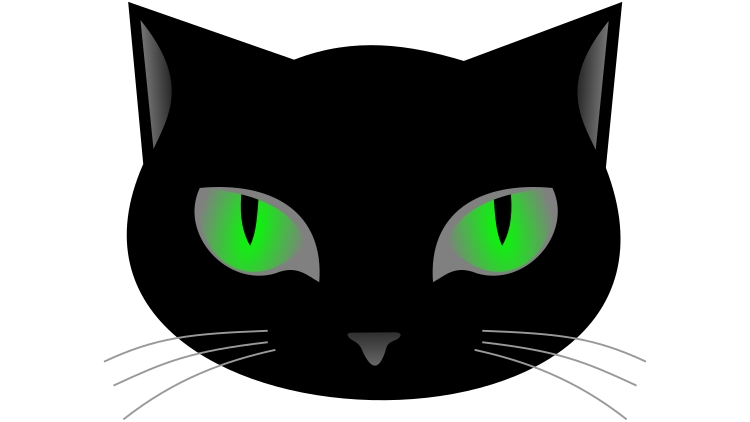
\includegraphics[width=1.2\textwidth, height=0.40\textheight]{figures/logo_picat_alex.jpg}
\end{center}
\end{figure}
\end{minipage}
\end{frame}
%%%%%%%%%%%%%%%%%%%%%%%%%%


\begin{frame}[fragile,allowframebreaks=0.8,c]
	\frametitle{Predicados e Funções}
    
\begin{itemize}

\item Os \textbf{predicados} sempre assumem valores valores lógicos \texttt{true} ($1$) ou \texttt{false} ($0$).

\item Os \textbf{predicados} em seus argumentos, podem passar $n$-termos e receber
outros termos.

\item Quanto as \textbf{funções}, estas funcionam seguindo as regras de funções matemáticas,
sempre retornando um único valor

\item Predicados e funções são definidos com regras de \textit{casamento de padrões}


\item Predicados são conhecidos como \textbf{regras lógicas}, há dois tipos de regras:
\framebreak        
        \begin{itemize}
            \item Regras \textbf{sem} {\em backtracking} (\textit{non-backtrackable}):
        	
            \begin{tabbing}
              aa \= aaa \= aaa \= aaa \= aaa \= aaa \= aaa \kill
             \> \> \verb+ Cabeça , Condicional + \textbf{\textcolor{red}{=>}} \verb+ Corpo .+
            \end{tabbing}
            

            \item Regras \textbf{com} {\em backtracking}:
            
            \begin{tabbing}
              aa \= aaa \= aaa \= aaa \= aaa \= aaa \= aaa \kill
             \> \> \verb+ Cabeça , Condicional + \textbf{\textcolor{red}{?=>}} \verb+ Corpo .+
            \end{tabbing}
        
        \end{itemize}
\framebreak        
       
  \item A identificação da sintaxe é dada por:
  
  \begin{itemize}
  
      \item \emph{Cabeça}: indica um padrão de regra a ser casada.
      
      Forma geral:
      \begin{tabbing}
          aa \= aaa \= aaa \= aaa \kill
          \> \> $regra(termo_1, \ldots,termo_n)$
      \end{tabbing}
      
      Onde:
      
      \begin{itemize}
          \item \emph{regra} é um átomo que define o nome da regra.
          \item \emph{n} é a aridade da regra (\emph{i.e.} o total de argumentos)
          \item Cada \emph{$termo_i$} é um argumento da regra.
      \end{itemize}
      
      \item \emph{Cond}: é uma ou várias condições sobre a execução desta regra.
          
      \item \emph{Corpo}: define as ações da regra 
      
  \end{itemize}
  
  \item Todas as regras são finalizadas por um ponto final (.), seguido por um espaço 
  em branco ou nova linha.
  
  \item Ao longo dos exemplos, detalhes a mais sobre esta construção de \textbf{predicados} e \textbf{funções}
      
\end{itemize}

\end{frame}
%%%%%%%%%%%%%%%%%%%%%%%%%%%%%%%%%%%%%%%%%%%%%%%%%%%%%%%%%%%%%%%%%%%%%


\begin{frame}[fragile]
	\frametitle{Regras com e sem Backtracking -- Exemplo}


\begin{footnotesize}
\begin{verbatim}
main => regra_01(7)  ,
        regra_01(-4) ,
        regra_01(44) .
        
regra_01(0)          ?=> printf("\n  CHEGOU A 0 !!!\n").
regra_01(N) , N < 0  ?=> printf("\n  EH UM NEGATIVO !!!\n").
regra_01(N) , N > 10 ?=> printf("\n  EH MAIOR QUE 10 !!!\n").
regra_01(N) , N <= 10  =>  
          printf("\t :%d ", N),
          regra_01(N-1).

%% =<  EH IGUAL a >= :: sobrecarga
%%% $ picat regras_com_sem_backtraking.pi

\end{verbatim}

\end{footnotesize}
\textcolor{red}{Há uma recursão aqui. Algumas seções a frente.}

\end{frame}


%%%%%%%%%%%%%%%%%%%%%%%%%%%%%%%%%%%%%%%%%%%%%%%%%%%%%%%%%%%%%%%%%%%%%

\subsection{Casamento de Padrões}

\begin{frame}[fragile]
\frametitle{Casamento de Padrões}

\begin{itemize}

\item O algoritmo de {\em casamento de padrões} para regras é análogo ao algoritmo de    unificação para variáveis. 

\item O objetivo é encontrar dois padrões que possam ser unificados para se inferir alguma ação.

\pause
\item Muitos exemplos no curso

\end{itemize}
\end{frame}


%%%%%%%%%%%%%%%%%%%%%%%%%%%%%%%%%%%%%%%%%%%%%%%%%%%%%%%%%%%%%%%%%%%%%

\begin{frame}[fragile]
\frametitle{Casamento de Padrões -- Procedimento}


Procedimento de {\em casamento de padrões}:

\begin{itemize}
	\item Dado um padrão $p_1(t_1, \ldots,t_m)$, este \emph{casa} 
	com um padrão semelhante $p_2(u_1, \ldots,u_n)$ se:
    
    \begin{itemize}
    	\item $p_1$ e $p_2$ forem átomos equivalentes;
    
        \item O número de termos (chamado de aridade) em ($t_1, \ldots,t_m$)
        e ($u_1, \ldots,u_n$) for equivalente.
    
    	\item Os termos ($t_1, \ldots,t_m$) e ($u_1, \ldots,u_n$) são equivalentes, ou tornaram-se  equivalentes pela unificação de variáveis	em qualquer um dos dois termos;
    \end{itemize}
    
    \item Caso essas condições forem satisfeitas, o padrão $p_1(t_1,\ldots,t_m)$  casa com o padrão $p_2(u_1, \ldots,u_n)$.
    
\end{itemize}        

\end{frame}

%%%%%%%%%%%%%%%%%%%%%%%%%%%%%%%%%%%%%%%%%%%%%%%%%%%%%%%%%%%%%%%%%%%%%

\begin{frame}[fragile]
    
\begin{block}{Exemplos de \textit{casamento}}

\begin{enumerate}
	\item A regra $fatorial(Termo, Resultado)$ pode casar com:\\
    $fatorial(1,1)$, $fatorial(5,120)$, $fatorial(abc,25)$, $fatorial(X,Y)$, \emph{etc}.
    
    \pause
     \item A regra $fatorial(Termo, Resultado), Termo \geq 0$ pode casar com:\\
    $fatorial(1,1)$, $fatorial(5,120)$, $fatorial(X,Y)$, $fatorial(Z,Z)$, \emph{etc}.
    
    \pause
    \item A regra $pai(X,Y)$ pode casar com:\\
    $pai(rogerio, miguel)$, $pai(rogerio, henrique)$, $pai(salomao, X)$, $pai(12,24)$, \emph{etc}.
    
    \pause
    \item A regra $pai(salomao, X)$ pode casar com:\\
    $pai(salomao, rogerio)$, $pai(salomao, fabio)$.
    
    \pause
    \item A regra $pai(salomao, fabio)$ pode casar com:\\
    $pai(X, fabio)$, $pai(salomao, X)$, $pai(X,Y)$
\end{enumerate}

\end{block}
    
\end{frame}

%%%%%%%%%%%%%%%%%%%%%%%%%%%%%%%%%%%%%%%%%%%%%%%%%%%%%%%%%%%%%%%%%%%%%

\begin{frame}[fragile]

	\frametitle{Metas ou Provas -- (\textit{goals})}
	
	\begin{itemize}
	    
	 \item Na matemática ao se deduzir um valor de um teorema, tem-se uma \textit{prova}. 
	  Assim, o termo  \textit{goal} eventualmente é chamado de \textit{prova do programa}
	 
	 \pause
	    \item Metas ou Provas (do inglês: \textit{goal}) são estados que definem o final da execução.
	    
  	 \pause
	    \item Uma meta pode ser, entre outros, um valor lógico, uma chamada de outra regra, 
	    uma exceção ou uma operação lógica.
	\end{itemize}

\end{frame}
    
  %  \begin{enumerate}
  %      \item \texttt{true, yes} $\Rightarrow$ Valor lógico para verdade.
%   %      \item \texttt{false, no} $\Rightarrow$ Valor lógico para falsidade.
%         \item \texttt{$p(t_1,\ldots,t_n)$} $\Rightarrow$ Chamada de uma regra \emph{p}.
%         \item \texttt{(P,Q), (P;Q), (P\&\&Q), (P||Q), not P} $\Rightarrow$ Operação lógica 
%     %    sobre uma ou mais metas P e Q.
   % \end{enumerate}
%%%%%%%%%%%%%%%%%%%%%%%%%%%%%%%%%%%%%%%%%%%%%%%%%%%%%%%%%%%%%%%%%%%%%
\subsection{Funções}

\begin{frame}[fragile]
	\frametitle{Funções -- I}
    
    \begin{itemize}
        \item A forma geral de uma função é:
        
        \begin{tabbing}
          aa \= aaa \= aaa \= aaa \= aaa \= aaa \= aaa \kill
          \> \> $Cabe$ç$a = X \ $\verb+=>+$\ Corpo$. 
        \end{tabbing}

       \pause        
        \item Caso tenhamos uma condição \emph{Cond}::
        
        \begin{tabbing}
          aa \= aaa \= aaa \= aaa \= aaa \= aaa \= aaa \kill
          \> \> $Cabe$ç$a = X , Cond \ $\verb+=>+$\ Corpo$. 
        \end{tabbing}
        
        \item \textcolor{red}{Funções \textbf{não} admitem \textbf{\textit{backtracking}}}.
    \end{itemize}
\end{frame}
    
\begin{frame}[fragile]
	\frametitle{Funções -- II}

    
    \begin{itemize}
        \item Funções são tipos especiais de regras que sempre sucedem com \emph{uma} 
        resposta.
        
        \pause
        \item Funções em Picat tem como intuito serem sintaticamente semelhantes a funções matemáticas (vide \emph{Haskell}).
        
        \pause
        \item Em uma função a \emph{Cabeça} é uma equação do tipo $f(t_1,\ldots,t_n)=X$, onde
        \emph{f} é um átomo que é o nome da função, \emph{n} é a aridade da função, e cada
        termo $t_i$ é um argumento da função.
        
        \item \emph{X} é uma expressão que é o retorno da função.
        
    \end{itemize}
    
\end{frame}
    
\begin{frame}[fragile]
	\frametitle{Funções  -- III}
    
    \begin{itemize}
    
        \item Funções também podem ser denotadas como fatos, onde podem servir como 
        \textbf{\textit{aterramento}} para regras recursivas.
        %, ou até mesmo como versões simplificadas de uma      regra. 
        
        
        \item Esta são denotadas como: $f(t_1,\ldots,t_n) = $ \emph{Expressão}, onde \textit{Expressão}
        pode ser um valor ou uma série de ações.
        
    \end{itemize}
    
\end{frame}

%%%%%%%%%%%%%%%%%%%%%%%%%%%%%%%%%%%%%%%%%%%%%%%%%%%%%%%%%%%%%%%%%%%%%
\begin{frame}[fragile]
\frametitle{Regras, Metas e Funções -- Exemplo}

\begin{footnotesize}
\begin{verbatim}
main =>
       X = 3, 
       Y = 4,
       um_predicado(X,Y,Z),
       R = uma_funcao(X,Y),
       printf("\n Z: %d \t R: %d", Z, R),
       println("\n FIM"). 
       
um_predicado(X,Y,Z) => Z = X + Y.

uma_funcao(X,Y) = R => R = X + Y.
\end{verbatim}

\end{footnotesize}
\end{frame}


\begin{frame} [fragile]

\frametitle{Regras, Metas e Funções -- Exemplo}
\begin{footnotesize}
\begin{verbatim}
Picat> cl('predicados_funcoes').
Compiling:: predicados_funcoes.pi
predicados_funcoes.pi compiled in 0 milliseconds
loading...

yes

Picat> um_predicado(3,4,Z), write(Z).
7Z = 7
yes

Picat> uma_funcao(3,4) = R, write(R).
7R = 7
yes

Picat>
\end{verbatim}
\end{footnotesize}
\end{frame}

%%%%%%%%%%%%%%%%%%%%%%%%%%%%%%%%%%%%%%%%%%%%%%%%%%%%%%%%%%%%%%%%%%%%%

\subsection{Relembrando as Regras}
\begin{frame}[c, fragile, allowframebreaks=0.75]
	\frametitle{Relembrando as Regras}
    
    \begin{itemize}
        \item Forma geral de um predicado do tipo Regra:
    
        \begin{tabbing}
          aa \= aaa \= aaa \= aaa \= aaa \= aaa \= aaa \kill
          \> \> \verb+ Cabeça , Condicional  =>   Corpo .+ 
        \end{tabbing}
        
        \item  Forma geral de um predicado com \textit{backtracking}:
        
        \begin{tabbing}
          aa \= aaa \= aaa \= aaa \= aaa \= aaa \= aaa \kill
            \> \> \verb+ Cabeça , Condicional + \textbf{\textcolor{red}{?=>}} \verb+ Corpo .+
        \end{tabbing}
    \end{itemize}
    
    \textcolor{red}{Em Prolog, esta condicional (Cond) entra no corpo da regra. Picat é flexível!}

    \framebreak
    
    \begin{itemize}
        \framebreak
        
        \item Dentro de uma regra, \emph{Cond} só pode ser avaliado uma vez, acessando somente termos dentro do escopo do predicado.
        
        \item Sempre estar atento que: regras são \textbf{sempre avaliados com valores lógicos} ({\em true} ou {\em false})
        
        \item Por outro lado, as variáveis  como argumento ou  instanciadas
        dentro dele, podem ser utilizadas dentro do escopo da regra, 
        ou no escopo onde  esta regra foi chamada.
    \end{itemize}
    
\end{frame}

%%%%%%%%%%%%%%%%%%%%%%%%%%%%%%%%%%%%%%%%%%%%%%%%%%%%%%%%%%%%%%%%%%%%%

\subsection{Regras do Tipo  Fatos}
\begin{frame}[c,allowframebreaks=0.6,fragile]
\frametitle{Regras do Tipo  Fatos}

    \begin{itemize}
        \item As regras que não tem condicionais e nem corpo, estes  são conhecidos
        como:  \textit{fatos} ou \textit{regras sem-corpo}
        
       \item Estes \textit{fatos} são regras \textit{sempre verdadeiras}
        
        \item Formato dos fatos são do tipo:
        
        \begin{tabbing}
          aa \= aaa \= aaa \= aaa \= aaa \= aaa \= aaa \kill
          \> \> $p(t_1,\ldots,t_n)$. 
        \end{tabbing}
        
        \item Os argumentos de um \emph{fato} \textbf{não} podem conter \textbf{variáveis}.
        
        \framebreak
        
        \item A declaração de um fato é precedida por uma declaração \textbf{\emph{index}},
        algo como:
        
        \begin{tabbing}
        aa \= aaa \= aaa \= aaa \= aaa \= aaa \= aaa \kill
            \> \texttt{index ($M_{11},M_{12},\ldots,M_{1n}$) $\ldots$ ($M_{m1},M_{m2},\ldots,M_{mn}$)}\index{\texttt{index}} 
        \end{tabbing}
        
        \item Onde um $M_{ij}$ com o simbolo `$+$',  significa que este termo já foi 
        indexado.
        
        \item Quanto o `$-$' significa que este termo deve ser indexado
        
        \item Ou seja, quando ocorre um simbolo `$+$' em um grupo do \textit{index}, é avaliado
        pelo compilador como um valor constante a ser casada
        
        %, que não irá gerar uma nova regra durante
        %a execução do programa.
        
        \item Quanto ao `$-$', este é avaliado pelo compilador com uma variável que deverá ser 
        instanciada à um valor. Ou seja, quando se deseja unificar um valor a esta variável
        
        \item Dica: o parâmetro `$-$' no \textit{index} é quase como regra geral
                
        \item \textbf{Não} pode haver um \textbf{predicado} e um \textbf{predicado 
        fato} com \textbf{mesmo nome}.
        
    \end{itemize}
\end{frame}



\begin{frame} [fragile]
\frametitle{Exemplo -- Função e Regras}

\begin{footnotesize}
\begin{verbatim}
index (+,+,+) (+,+, -) (-,+,-) (-,-,+) (-,-, +) 
      (+,-,+) (+,+,-)  (-,-,-)
%(-,-,-) %% NENHUM argumento instanciao -- UTIL
%(+,+,+) %% TODOS ARGUMENTOS DEVEM ESTAR INSTANCIADOS
%(+,+, -) (-,+,-) (-,-,+) (-,-, +) (+,-,+) (+,+,-) (-,-,-)

and2(true,true,true).
and2(true,false,false).
and2(false,true,false).
and2(false,false,false).

main ?=>
       and2(X,Y,Z), % and eh reservado
       printf("\n X: %w \t Y: %w \t Z: %w", X, Y, Z),
       fail.
main =>       
       println("\n FIM"). 
\end{verbatim}
\end{footnotesize}

\textcolor{red}{Este exemplo é muito interessante. Execute ele na console do interpretador
excluindo alguns dos parâmetros do \textit{index}}

\end{frame}


%%%%%%%%%%%%%%%%%%%%%%%%%%%%%%%%%%%%%%%%%%%%%%%%%%%%%%%%%%%%%%%%%%%%%


%%%%%%%%%%%%%%%%%%%%%%%%%%%%%%%%%%%%%%%%%%%%%%%%%%%%%%%%%%%%%%%%%%%%%

\subsection{Exemplos}

\begin{frame}[fragile]

\frametitle{Exemplos}

\begin{block}{Exemplo de Predicado ou regra}
   
\begin{lstlisting}[frame=single]
contas_P0(X1, X2, X3, Z) ?=>
    number(X1),
    number(X2),
    number(X3),
    X1 < X2,
    X2 < X3,
    Z  =  (X2 + X3).
    
contas_P0(X1, _, _, Z) =>
   Z = X1.    
\end{lstlisting}
    \end{block}

        
\end{frame}

\begin{frame}[fragile]

\begin{block}{Exemplo de Funções}
     
\begin{lstlisting}[frame=single]
contas_F0(X1, X2, X3) = Z, (number(X1), 
                           number(X2), 
                           number(X3)) =>
    if (X1 < X2 && X2 < X3) then
    Z  =  (X2 + X3)
    else
    Z  =  X1
    end.
\end{lstlisting}
        
 \end{block}

\textcolor{red}{\textit{Aperitivo} à próxima seção: condicionais e laços!}
    
\end{frame}    
\begin{frame}[fragile]
   
\begin{block}{Mais Exemplos (Fatos e Regras)}
    
\begin{lstlisting}[frame=single]
index(-,-) (+,-) (-,+)
pai(salomao, rogerio).
pai(salomao, fabio).
pai(rogerio, miguel).
pai(rogerio, henrique).

avo(X,Y) ?=> pai(X,Z), pai(Z,Y).
irmao(X,Y) ?=> pai(Z,X), pai(Z,Y).
tio(X,Y) ?=> pai(Z,Y), irmao(X,Z).
\end{lstlisting}
    
 \end{block}
    
\end{frame}    
%%%%%%%%%%%%%%%%%%%%%%%%%%%%%%%%%%%%%%
\begin{frame}[fragile]
    
\begin{block}{Exemplos de Funções -- Equivalentes}
    
\begin{lstlisting}[frame=single]
eleva_cubo(1) = 1.
eleva_cubo(X) = X**3.
eleva_cubo(X) = X*X*X.
eleva_cubo(X) = X1 => X1 = X**3.
eleva_cubo(X) = X1 => X1 = X*X*X.
\end{lstlisting}
        
\end{block}
    
\end{frame}

%%%%%%%%%%%%%%%%%%%%%%%%%%%%%%%%%%%%%%%%%%%%%%%%%%%%%%%%%%%%%%%%%%%%%
%%% ATE AQUI
\section{Comandos Condicionais, Laços e Repetições}

\begin{frame}[fragile]
\frametitle{Comandos Condicionais, Laços e Repetições}
    
  
  \begin{itemize}
      
      \item Ao contrário do Prolog, Picat apresenta
      conceitos e comandos da programação imperativa
      
      \pause
      \item Esta maneira  ameniza os obstáculos
      em se aprender uma linguagem com o paradigma lógico,
      tendo outros elementos conhecidos
  
          \pause
      \item Assim, Picat apresenta estruturas clássicas
      como: 
      \begin{itemize}
        \item  \texttt{if--then--end}, \texttt{if--then--else--end}, \texttt{if--then--elseif--then--....end}
        \item  \texttt{foreach}
        \item  \texttt{while}
        \item  \texttt{do--while}
        \item Bem como a atribuição, `\texttt{:=}', já discutida
      \end{itemize}
   \end{itemize}

       
\end{frame}    
     
    %%%%%%%%%%%%%%%%
    
\begin{frame}[fragile]
\frametitle{Comandos Condicionais}
    
    \begin{itemize}
        
        \item Picat implementa uma  estrutura condicional explícita (na programação em lógica, voce faz isto implicitamente)
        
        \pause
        \item Sua notação é:\\
        
        \begin{tabbing}
            aa \= aaa \= aaa \= aaa \= aaa \= aaa \= aaa \kill
            \> \texttt{if (Exp) then}\\
            \> \> \texttt{Ações} \\
            \> \texttt{else}\\
            \> \> \texttt{Ações}\\
            \> \vdots\\
            \> \texttt{end} 
        \end{tabbing}
        
        \pause
        \item Onde \emph{Exp} é uma expressão lógica  avaliada como verdadeira ou  falsa.
     
     \pause   
        \item A última ação antes de um \emph{else} ou \emph{end} não deve ter  vírgula nem ponto e vírgula ao final da linha.
  
     \pause   
        \item Tem-se ainda o \texttt{elseif} que pode estar embutido no comando \texttt{if--then--else--end}
        
    \end{itemize}
\end{frame}    
    
    
    
    
    
    
    
    
\begin{frame}[fragile]

\begin{block}{Exemplo: \texttt{if--then--else--end} }
     
\begin{lstlisting}[frame=single]
    ,
if (X <= 100) then
        println("X e menor que 100")
    elseif (X <= 1000 && X >= 500) then
        println("X estah entre 500 e 1000")
    else
        println("X estah abaixo de  500")
    end
    ,
\end{lstlisting}
        
\end{block}
\end{frame}    

    
    
%%%%%%%%%%%%%%%%%%%%%%%%%%%%%%%%%%%%%%%%%%%%%%%%%%%%%%%%%%%%%%%    
    
    
    
\begin{frame}[fragile]
\frametitle{Estruturas de Repetições}
       

\begin{itemize}
    
    \item Picat também implementa 3 estruturas de repetição, são elas:
    \texttt{foreach}, \texttt{while}, e \texttt{do-while}.
    
    \pause
    \item O laço do  \texttt{foreach}  itera sobre termos simples e compostos.
    
        \pause
    \item O  \texttt{while} repete um conjunto de ações enquanto uma 
     condição for verdadeira.
     
        \pause
    \item A condição pode ser simples ou combinada
     
     
        \pause
    \item O laço \texttt{do-while} é análogo ao  \texttt{while}, porém ele 
    sempre executa pelo menos uma vez.
\end{itemize}
\end{frame}    


%%%%%%%%%%%%%%%%%%%%%%%%%%%%%%%%%%%%%%%%%%%%%%%%%%%%%%%%%%%%%%%    
\begin{frame}[fragile]
\frametitle{Estruturas de Repetições: \texttt{foreach}}

    \begin{itemize}
        \item Um laço \texttt{foreach} tem a seguinte forma:
        
        \begin{tabbing}
            aa \= aaa \= aaa \= aaa \= aaa \= aaa \= aaa \kill
            \> \texttt{foreach ($E_1$ in $D_1$, $Cond_1$, $\ldots$, $E_n$ in $D_n$, $Cond_n$)}  \\
            \> \> $Metas$ \\
            \>  \texttt{end} 
        \end{tabbing}
    
   \pause    
   Esta notação é dada por:
        
    \item  $E_i$ é um \emph{padrão de iteração} ou \emph{iterador}. 
        
    \item  $D_i$ é  uma expressão de \emph{valor composto}. Exemplo: uma lista de valores
        
     \item  $Cond_i$ é uma condição opcional sobre os iteradores $E_1$ até $E_i$.
        
     \item Laços do \texttt{foreach} podem conter múltiplos iteradores. 
     Caso isso ocorra, o compilador interpreta isso como diversos laços aninhados.
        
        % Maiores detalhes, ver Manual do Usuário. % copiar para outros slides
        
        % Exemplo 1 iterador e multiplos iteradores
        
    \end{itemize}
\end{frame}    


\begin{frame}[fragile]

\begin{block}{Exemplo: \texttt{foreach} }
     
\begin{lstlisting}[frame=single]
    
laco_01 =>  
    L = [17, 3, 41, 25, 8, 1, 6, 40],  
    foreach (E in L)  
        println(E)  
    end.  
\end{lstlisting}
        
\end{block}
\end{frame}    


%%%%%%%%%%%%%%%%%%%%%%%%%%%%%%%%%%%%%%%%%%%%%%%%%%%%%%%%%%%%%%%    
\begin{frame}[fragile]
\frametitle{Estruturas de Repetições: \texttt{while}}


\begin{itemize}
        \item O laço do \texttt{while} tem a seguinte forma:
        
        \begin{tabbing}
            aa \= aaa \= aaa \= aaa \= aaa \= aaa \= aaa \kill
            \> \texttt{while ($Cond$)} \\
            \> \> $Metas$  \\
            \>  \texttt{end}
        \end{tabbing} 
        
        \item Enquanto a expressão lógica \emph{Cond} for verdadeira, o conjunto de \texttt{Metas} é executado.
        
\end{itemize}
\end{frame}    


\begin{frame}[fragile]

\begin{block}{Exemplo: \texttt{while} }
     
\begin{lstlisting}[frame=single]
  
laco_02 =>  
    I = 1,  
    while (I <= 9)  
        println(I),  
        I := I + 2  
    end.  
\end{lstlisting}
        
\end{block}
\end{frame}    

%%%%%%%%%%%%%%%%%%%%%%%%%%%%%%%%%%%%%%%%%%%%%%%%%%%%%%%%%%%%%%%    
\begin{frame}[fragile]
\frametitle{Estruturas de Repetições: \texttt{do-while}}

    \begin{itemize}
        
        \item O laço \texttt{do-while} tem a seguinte forma:
        
        \begin{tabbing}
            aa \= aaa \= aaa \= aaa \= aaa \= aaa \= aaa \kill
            \> \texttt{do} \\
            \> \> $Metas$  \\
            \>  \texttt{while ($Cond$)}
        \end{tabbing} 
        
        \item Ao contrário do  \texttt{while} o iterador \texttt{do-while}
        vai executar \texttt{Metas} pelo menos uma vez antes de avaliar \texttt{Cond}.
        
    \end{itemize}
    
\end{frame}


\begin{frame}[fragile]

\begin{block}{Exemplo: \texttt{do-while} }

\begin{lstlisting}[frame=single]
     
laco_03 =>  
     J = 6,  
    do  
        println(J),  
        J := J + 1  
    while (J <= 5).  
\end{lstlisting}
        
\end{block}
\end{frame}    


%%%%%%%%%%%%%%%%%%%%%%%%%%%%%%%%%%%%%%%%%%%%%%%%%%%%%%%%%%%%%%%%%%%%%

\subsection{Funções e Predicados Especiais}


\begin{frame}[fragile]
%[c,allowframebreaks]

\frametitle{Funções e Predicados Especiais}
    % Compreensão de lista
    % Entrada e Saida de Dados
\begin{itemize}
    
    \item Há algumas funções e predicados especiais em Picat 
    que necessitam de algum cuidado.
    
    \pause
    \item São elas: \texttt{compreensão de listas/vetores}, 
    \texttt{entrada de dados} e \texttt{saída de dados}.
    
    \item Na verdade, já fizemos uso delas, porém sem a ênfase de que
    são funções ora predicados.
    
\end{itemize}
\end{frame}      


%%%%%%%%%%%%%%%%%%%%%%%%%%%%%%%%%%%%%%%%%%%%%%%%
\begin{frame}[c,allowframebreaks]

\frametitle{Compreensão de Listas e Vetores}    
    
\begin{itemize}    
    \item A função de \underline{\textit{compreensão de listas e vetores}} é uma função especial que  permite a fácil criação de listas ou vetores, opcionalmente seguindo uma regra de 
    criação.
    
    \item Sua notação é:
    
    \begin{tabbing}
        aa \= aaa \= aaa \= aaa \= aaa \= aaa \= aaa \kill
        \> \> \texttt{[$T$ : $E_1$ \texttt{in} $D_1$, $Cond_1$, $\ldots$, $E_n$ in $D_n$, $Cond_n$]} 
    \end{tabbing}
    
    \item Onde, $T$ é uma expressão  adicionada a lista, cada $E_i$ é um 
    iterador, cada $D_i$ é um termo composto ou expressão que gera um termo composto, e cada $Cond_i$ é uma condição sobre cada iterador de $E_1$ até $E_i$.
    
    \item Há uma seção dedicada a listas. Voltaremos ao assunto.
    
    \framebreak

    \item Esta função pode gerar um vetor também, a notação é um pouco diferente:
    
    \begin{tabbing}
        aa \= aaa \= aaa \= aaa \= aaa \= aaa \= aaa \kill
        \> \> \texttt{\{$T$ : $E_1$ \texttt{in} $D_1$, $Cond_1$, $\ldots$, $E_n$ in $D_n$, $Cond_n$\}} 
    \end{tabbing}
    
    \item Neste caso, os delimitadores são $\{$ e $\}$ de um vetor

\end{itemize}

\end{frame}      

% %%%%%%%%%%%%%%%%%%%%%%%%%%%%%%%%%%%%%%%%%    
 \begin{frame}[fragile]
 \frametitle{Compreensão de Listas e Vetores: Exemplo}
\begin{footnotesize}

\begin{verbatim}
main =>
 L = [(A, I) : A in [a, b], I in 1 .. 2],
 V = {(I, A) : A in [a, b], I in 1 .. 2},
 printf("\nL: %w  \nV: %w\n", L, V),
 imp_vetor(V).

imp_vetor (M) => 
Tam = M.length,  %% tamanho de M
  nl,
   foreach(I in 1  .. Tam )
     printf("V(%d):%w \t" , I, M[I] )
    end,
  nl.
%%%% $picat vetor_exemplo_01.pi
\end{verbatim}

\end{footnotesize}
 
\end{frame}


%%%%%%%%%%%%%%%%%%%%%%%%%%%%%%%%%%%%%%%%%%%%%%%%%%%%%%
\begin{frame}[c,allowframebreaks]

\frametitle{Leitura e Escrita}    

\begin{itemize}
        
\item Picat tem diversas variações  funções de leitura de valores,
        que serve tanto para ler de uma console \texttt{stdin},
        como de um arquivo qualquer.
        
\item Aos usuários de Prolog, aqui não precisamos do delimitador
final de `\textbf{.}'   ao final de uma leitura. 

\item Válido quando editamos no interpretador, o `\textbf{.}' final é opcional
        
\framebreak        
\item As mais importantes são:

\begin{itemize}
  
  \item \texttt{read\_int($FD$) = $Int$} $\Rightarrow$ Lê um \textit{Int} do 
  arquivo $FD$.
  
  \item \texttt{read\_real($FD$) = $Real$} $\Rightarrow$ Lê um \textit{Float} do 
  arquivo $FD$.
  
  \item \texttt{read\_char($FD$) = $Char$} $\Rightarrow$ Lê um \textit{Char} do 
  arquivo $FD$.
  
  \item \texttt{read\_line($FD$) = $String$} $\Rightarrow$ Lê uma \textit{Linha} 
  do arquivo $FD$.
  
\end{itemize}

\item Caso se deseja ler da console, padrão \texttt{stdin}, $FD$, o nome do descritor de arquivo,  pode ser omitido.

\framebreak

\item Os dois predicados mais importantes para saída de dados, são 
\texttt{write} e \texttt{print}.

\item Cada um destes predicados tem três variantes, são eles:

\begin{itemize}

\item \texttt{write($FD$, $T$)} $\Rightarrow$ Escreve um termo $T$ no arquivo 
$FD$.

\item \texttt{writeln($FD$, $T$)} $\Rightarrow$ Escreve um termo $T$ no arquivo 
$FD$, e pula uma linha ao final do termo.

\item \texttt{writef($FD$, $F$, $A\ldots$)} $\Rightarrow$ Este predicado é usado 
para escrita formatada para um arquivo $FD$, onde $F$ indica uma série de 
formatos para cada termo contido no argumento $A\ldots$. O número de argumentos 
não pode exceder 10.

\end{itemize}
        
\framebreak
        
\item Analogamente, para o predicado \texttt{print}, temos:

\begin{itemize}

  \item \texttt{print($FD$, $T$)} $\Rightarrow$ Escreve um termo $T$ no arquivo 
  $FD$.
  
  \item \texttt{println($FD$, $T$)} $\Rightarrow$ Escreve um termo $T$ no arquivo 
  $FD$, e pula uma linha ao final do termo.
  
  \item \texttt{printf($FD$, $F$, $A\ldots$)} $\Rightarrow$ Este predicado é usado 
  para escrita formatada para um arquivo $FD$, onde $F$ indica uma série de 
  formatos para cada termo contido no argumento $A\ldots$. O número de argumentos 
  não pode exceder 10.

\end{itemize}

\item Caso queira escrever para \texttt{stdout}, o nome do  $FD$, pode ser omitido.

\end{itemize}
    
\end{frame}

%%%%%%%%%%%%%%%%%%%%%%%%%%%%%%%%%%%%%%%%%%%%%%%%%%%%%%%%%%%%%%%%%%%%%

\begin{frame}
{Tabela de Formatação para Escrita}

Apenas os mais importantes, há outros como: hexadecimal, notação científica,
etc. Ver no apêndice do Guia do Usuário.    
\begin{table}[h]
    \begin{tabular}{l|l}
        \hline  \hline
        \textbf{Especificador} & \textbf{Saída} \\
        \hline 
        \hline 
        \texttt{\%\%} & Sinal de Porcentagem \\
        \texttt{\%c} & Caráctere \\
        \texttt{\%d \%i} & Número Inteiro Com Sinal \\
        \texttt{\%f} & Número Real \\
        \texttt{\%n} & Nova Linha \\
        \texttt{\%s} & \textit{String} \\
        \texttt{\%u} & Número Inteiro Sem Sinal \\
        \texttt{\%w} & Termo \textbf{qualquer} \\
        \hline   \hline
    \end{tabular}
\end{table}
\end{frame}

%%%%%%%%%%%%%%%%%%%%%%%%%%%%%%%%%%%%%%%%%%%%%%%%%%%%%%%%%%%%%%%%%%%%%

\begin{frame}

\frametitle{Comparação entre \texttt{write} e \texttt{print}}
     
\begin{table}[h]
    \centering
    \begin{tabular}{ l|l|l|l }
        \hline         \hline
        Dados $\Rightarrow$  & "abc" & [a,b,c] & 'a@b'\\
        \hline         \hline
        \texttt{write}   & [a,b,c] & [a,b,c] & 'a@b' \\
        \hline
        \texttt{writef}  & [a,b,c] (\%s) & abc (\%w) & 'a@b' (\%w) \\
        \hline
        \texttt{print}   & abc & abc & a@b \\
        \hline
        \texttt{printf}  & abc (\%s) & abc (\%w) & a@b (\%w) \\ 
        \hline \hline
    \end{tabular}
\end{table}

\end{frame}

%%%%%%%%%%%%%%%%%%%%%%%%%%%%%%%%%%%%%%%%%%%%%%%%%%%%%%%%%%%%%%%%%%%%%

\begin{frame}[fragile]

\frametitle{Exemplos}
    
    \begin{block}{Condicionais}
        \begin{lstlisting}[frame=single]
main =>
    X = read_int(),
    if(X <= 100)then
        println("X e menor que 100")
    else
        println("X nao e menor que 100")
    end.
.
        \end{lstlisting}
    
    \end{block}
\end{frame}

\begin{frame}[fragile]

\frametitle{Exemplos -- Repetições}
    
   \begin{lstlisting}[frame=single]
main =>
    X = read_int(),
    println(x=X),
    while(X != 0)
        X := X - 1,
        println(x=X)
    end
.
   \end{lstlisting}
        
   \begin{lstlisting}[frame=single]
main =>
    X = read_int(),
    Y = X..X*3,
    foreach(A in Y)
        println(A)
    end.
        \end{lstlisting}
    
\end{frame}

\begin{frame}[fragile]
\frametitle{Exemplos -- Compreensão de Listas}    
       
 \begin{lstlisting}[frame=single]
main => 
  Tamanho = read_int(),
  Y = [read_int() : 1..Tamanho],
  Z = {X : X in Y, X >= 0},
  forach(I in 1..Tamanho)
      if(Y[I] >= 0)then
          printf("Y[%d] e maior ou igual que 0\n",I)
      else
          printf("Y[%d] e menor que 0\n",I)
      end
  end
 printf("Os valores de Y que sao maiores que 0 sao:\n%w",Z)
.
\end{lstlisting} 
       
\textcolor{red}{Este exemplo reúne muitos conceitos desta seção.}       
   
\end{frame}

%%%%%%%%%%%%%%%%%%%%%%%%%%%%%%%%%%%%%%%%%%%%%%%%%%%%%%%%%%%%%%%%%%%%%

\begin{frame}[fragile]
\frametitle{Reflexões}

\begin{itemize}


  \item Esta seção  trata da sintaxe do Picat
  
    \pause
  \item Embora sua sintaxe não seja muito extensa, ela precisa 
  ser praticada
  
    \pause
  \item Como este conteúdo se assemelha as LPs clássicas, como exercício,
  voce está apto a fazer alguns algoritmos de outras linguagens.

  \pause
  \item Se antes o Prolog era complicado, com Picat,
  tudo ficou análogo a Python e a linguagem C
  
  \pause
  \item Em \url{https://github.com/claudiosa/CCS/tree/master/picat/input_output_exemplos}
  tem vários exemplos avançados de entradas e saídas 
  
  \pause
  \item Mãos à obra!
 
\end{itemize}

\end{frame}

%%%%%%%%%%%%%%%%%%%%%%%%%%%%%%%%%%%%%%%%%%%%%%%%%%%%%%%%%%%%%%%%%%%%%%%%%%%%%%%%%%%%

\section{Recursão}

\subsection{Recursão}
\begin{frame}[fragile]

\frametitle{Recursão}

\begin{itemize}

    \item A \textit{recursão} é um importante conceito da matemática e presente em muitas  linguagens
    de programação. Exemplo: LISP, Haskell, etc

    \pause
    \item Permite expressar conceitos complexos em uma sintaxe abstrata, mas  simples de ler.
    \pause
    \item Uma regra é dita recursiva quando ela faz auto-referência.
    
    \pause
    \item Em Picat, a recursão pode ser usada sob uma notação em \textit{lógica} ou \textit{funcional}
    
    \pause
    \item A funcional apresenta muita clareza ao código!
\end{itemize}

%\pause
%\centering
%
\includegraphics[scale=0.5]{figures/Recursao.png}
  
\end{frame}

%%%%%%%%%%%%%%%%%%%%%%%%%%%%%%%%%%%%%%%%%%%%%%%%%%%%%%%%%%%%%%%%%%%%%%%%

\begin{frame}[fragile]

\frametitle{Conceitos de Recursividade via Exemplos -- I}

\begin{block}{Somatório dos $N$ naturais}

 O somatório dos \emph{n}  primeiros  números naturais é recursivamente 
 definido como a soma de todos \emph{n-1} números, mais o termo \emph{n}. 
 Ou seja:

    \[
    S(n)=\left \{
    \begin{tabular}
        [c]{ll}
        $1$ & para $n=1$ \\
        $S(n-1) + n $ & para $n \geqslant 2$ e $n \in \mathbb{N}$
    \end{tabular}
    \right.
    \]
    
    Ou seja:
    
    \[
    S(n)=
    \begin{tabular}[c]{cc}
        $\underbrace{1+2+3+.....+(n-1)}$ &  $  + n$\\
        $S(n-1)$ &
    \end{tabular}
    \]
\end{block}            

\end{frame}

\begin{frame}[fragile]
\frametitle{Conceitos de Recursividade via Exemplos -- II}


\begin{block}{Fatorial}

O Fatorial de um número $n$ é definido  recursivamente pela
 multiplicação do fatorial do termo $n-1$ por $n$. 
  O fatorial só pode ser calculado para números positivos. 
  Adicionalmente, o fatorial de $0$ é igual a 
  $1$ por definição.
    \[ 
    Fat(n)=\left\{
    \begin{tabular}[c]{ll}%
        $1$ & para $n = 0$\\
        $Fat(n-1) . n$ & para $n\geqslant1$ e $n \in \mathbb{N}$
    \end{tabular}
    \right.
    \]
    
    Portanto:
    
    \[
    Fat(n)=
    \begin{tabular}
        [c]{cc}%
        $\underbrace{1\ast2\ast3 . ..... . (n-1)}$ & $ .  \ n$\\
        $Fat(n-1)$ &
    \end{tabular}
    \]

\end{block}    
\end{frame}


\begin{frame}[fragile]
\frametitle{Conceitos de Recursividade via Exemplos -- III}

\begin{block}{Sequência Fibonacci}

A sequência Fibonacci é uma sequência de números calculada a partir da soma dos
dois últimos números anteriores desta. Ou seja o $n-esimo$ termo da Sequência Fibonacci é definido como a soma dos termos $n-1$ e $n-2$. Como fato ou definição: os dois primeiros termos, $n = 0$ e $n = 1$, são respectivamente, $0$ e $1$.
      
      \[
      Fib(n)=\left\{
      \begin{tabular}[c]{ll}%
          $0$ & para $n = 0$\\
          $1$ & para $n = 1$\\
          $Fib(n-1) + Fib(n-2)$ & para $n\geqslant1$ e $n \in \mathbb{N}$
      \end{tabular}
      \right.
      \]
 
\end{block}    
\end{frame}

%%%%%%%%%%%%%%%%%%%%%%%%%%%%%%%%%%%%%%%%%%%%
\begin{frame}[fragile]

\frametitle{Conceitos de Recursividade via Exemplos -- IV}

  \begin{itemize}
      
      \item Podemos perceber algo em comum entre estas três regras, todas tem uma ou mais
      condições que sempre tem o mesmo valor de retorno, ou seja, todas tem uma \textit{regra de  aterramento}.
      
      \pause
      \item Uma condição de \textit{aterramento} é uma condição onde a chamada recursiva da regra
      acaba (pára ou termina).
      
       \pause
      \item Caso uma regra não tenha uma \textit{regra de aterramento}, poderá ocorrer uma recursão infinita deste regra, ou seja, são feitas infinitas chamadas recursivas
      da regra.
  \end{itemize}

\end{frame}

%%%%%%%%%%%%%%%%%%%%%%%%%%%%%%%%%%%%%%%%%%%%
\begin{frame}[fragile]

\frametitle{Exemplos}

Numa visão funcional, estas regras matemáticas podem ser transcritas em Picat como:

    \begin{lstlisting}[frame=single]
fatorial(0) = 1.
fatorial(1) = 1.
fatorial(n) = n * fatorial(n-1).
    \end{lstlisting}

    \begin{lstlisting}[frame=single]
fibonacci(0) = 0.
fibonacci(1) = 1.
fibonacci(n) = fibonacci(n-1) + fibonacci(n-2).
    \end{lstlisting}

    \begin{lstlisting}[frame=single]
somatorio(0) = 0.
somatorio(1) = 1.
somatorio(n) = n + somatorio(n-1).
    \end{lstlisting}

\end{frame}

%%%%%%%%%%%%%%%%%%%%%%%%%%%%%%%%%%%%%%%%%%%%%%%%%%%%%%%%%%%%%%%%%%%%%%%%%%%%%%

\begin{frame}[fragile]

\frametitle{Recursão Infinita}

    \begin{itemize}
        \item Caso a definição do fatorial fosse modificada para:
        
        \[
        Fat(n)= 
        \begin{tabular}[c]{ll}
            $Fat(n-1)\ast n$, &$\forall n \in \mathbb{N}$ ou $\forall n \geq 0$
        \end{tabular}
        \]
        \pause
        \item Teríamos um caso de \textit{recursão infinita}, pois a regra Fatorial continuaria
        a ser chamada com $n < 0$
        
        \item Nesse caso haveria um erro, pois estaria tentando executar algo indefinido.
        
    \end{itemize}

\end{frame}

%%%%%%%%%%%%%%%%%%%%%%%%%%%%%%%%%%%%%%%%%%%%%%%%%%%%%%%%%%%%%%%%%%%%%%%%%%%%%%


\begin{frame}[fragile]

\frametitle{Exercício}

Para os exemplos anteriores, reescreva-os
as formulações sob uma visão
\textit{lógica} e  \textit{procedural}.

\end{frame}


%%%%%%%%%%%%%%%%%%%%%%%%%%%%%%%%%%%%%%%%%%%%%%%%%%%%%%%%%%%%%%%%%%%%%%%%%%%%%%%%%%%%%%%%%%

\subsection{\textit{Backtracking}}
\begin{frame}[fragile]

\frametitle{\textit{Backtracking}}
\begin{itemize}
  \item O mecanismo de \textit{backtracking} é bem conhecido por algumas linguagens de programação

 % \pause 
 % \item Backtracking é um tipo de algoritmo que representa um refinamento da busca por força bruta,
%   em que múltiplas soluções podem ser eliminadas sem serem explicitamente examinadas.
  
  \pause 
  \item Em Picat, o \textit{backtracking} é controlável e é habilitado pelo símbolo
  \verb!?=>! no escopo da regra. 

\end{itemize}

\end{frame}

\begin{frame}[fragile]
\frametitle{Ilustrando o \textit{Backtracking} -- 01}

\begin{figure}[!htb]
\begin{center}
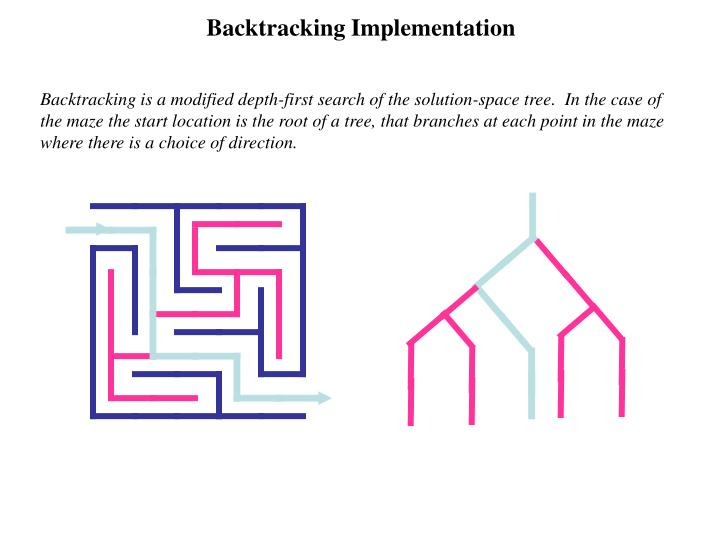
\includegraphics[width=0.80\textwidth, height=0.90\textheight]{figures/ilustra_backtracking_01.jpg}
%\caption{Realizar buscas com regiões reduzidas -- promissoras (regiões factíveis de soluções)}
\end{center}
\end{figure}
\end{frame}


\begin{frame}[allowframebreaks=0.7]
\frametitle{\textit{Backtracking}}

Basicamente o procedimento do \textit{Backtracking} é definido por:

\begin{enumerate}

\item Inicia-se por  um casamento de um predicado \textit{backtrackable} $p$ com um outro predicado $p$.

\item Segue-se a execução da regra $p$, executando a instância das variáveis da \underline{esquerda para direita}.
 \textbf{Exemplo} (ilustrativo):\\
      \texttt{p(X1,X2,X3, ....., Xn) ?=> q1(X1), q2(X2), ...., qn(Xn).} 

\item Caso ocorra uma falha durante a execução da regra $p$,
 o compilador busca re-instanciar as variáveis do corpo de $p$ que falharem. Esta tentativa segue uma ordem:\\ 
  $q1(X1) \rightarrow q2(X2)\rightarrow ....\rightarrow qn(Xn)$, até a variável $Xn$
%, incluindo aquelas indexadas a partir de um domínio.
%, com a única exceção sendo variáveis instanciadas a
%partir de argumentos do predicado.

\item Caso $Xn$ seja instanciada com sucesso, tem-se uma resposta consistente para $p$

\item No caso de uma falha completa na regra corrente $p$, segue-se para uma próxima regra $p$
 (\texttt{p ....?=> ...}), a qual  é avaliada com novas instâncias as suas  variáveis.

\item Este processo é completo (exaustivo) e se repete até não for mais possível a reinstanciação de variáveis, ou ocorrer uma falha  durante a   execução.
\end{enumerate}


\end{frame}


\begin{frame}[fragile]
\frametitle{Ilustrando o \textit{Backtracking} -- 02}

\begin{figure}[!htb]
\begin{center}
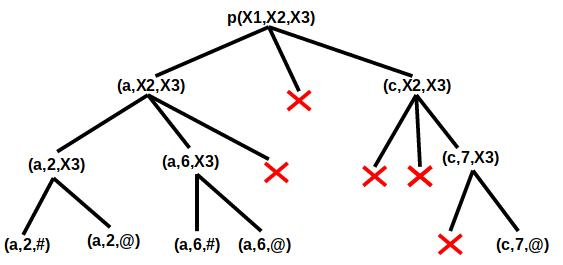
\includegraphics[width=0.950\textwidth, height=0.8\textheight]{figures/ilustra_backtracking_03.jpg}
%\caption{Realizar buscas com regiões reduzidas -- promissoras (regiões factíveis de soluções)}
\end{center}
\end{figure}
\textcolor{red}{Exercício: descubra os domínios possíveis de \texttt{X1}, \texttt{X2} e \texttt{X3}}
\end{frame}

s
\begin{frame}[fragile]
\frametitle{Ilustrando o \textit{Backtracking} -- 03}

\begin{figure}[!htb]
\begin{center}
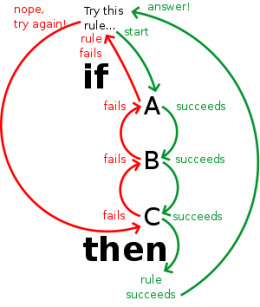
\includegraphics[width=0.60\textwidth, height=0.75\textheight]{figures/ilustra_backtracking_02.jpg}
%\caption{Realizar buscas com regiões reduzidas -- promissoras (regiões factíveis de soluções)}
\end{center}
\end{figure}

\end{frame}





%%%%%%%%%%%%%%%%%%%%%%%%%%%%%%%%%%%%%%%%%%%%%%%%%%%%%%%%%%%%%%%%%%%%%%%%%%%%%%%%%%%%%%%%%%

\begin{frame}[fragile]

\frametitle{Exemplos}
    
Tomando como exemplo uma relação de parentesco, como a seguinte:
% usar antecendente,sucessor, descendente etc.
        \begin{lstlisting}[frame=single]
index(-,-) (+,-) (-,+)
antecedente(ana,maria).
antecedente(pedro,maria).
antecedente(maria,paula).
antecedente(paula,lucas).
antecedente(lucas, eduarda).

index(-)
mulher(ana).
mulher(maria).
mulher(paula).
mulher(eduarda).
homem(pedro).
homem(lucas).

mae(X,Y) ?=> antecedente(X,Y), mulher(X).
pai(X,Y) ?=> antecedente(X,Y), homem(X).
avos(X,Y) ?=> antecedente(X,Z), antecedente(Z,Y).
sucessor(X,Y) ?=> antecedente(Y,X).
sucessor(X,Y) ?=> antecedente(Y,Z), sucessor(X,Z).
        \end{lstlisting}
    
\end{frame}


%%%%%%%%%%%%%%%%%%%%%%%%%%%%%%%%%%%%%%%%%%%%%%%%%%%%%%%%%%%%%%%%%%%%%%%%%%%%%%%%%%%%%%%%%%


\begin{frame}[fragile]
\frametitle{Exercícios}
    
    \begin{itemize}
        \item Uma chamada do tipo $mae(maria, X)$, seria como perguntar ao compilador
        "Maria é mãe de quem ?".
        
        \item Nesse caso o compilador iria testar cada possível valor que pudesse ser 
        unificado com $X$ que pudesse satisfazer a regra $mae(maria,X)$.
        
        \item Ou seja, seria como se estivéssemos perguntando:
        
        \begin{itemize}
            \item "Maria é mãe de Ana ?".
            
            \item "Maria é mãe de Paula ?".
            
            \item "Maria é mãe de Pedro ?".
            
    
        \end{itemize}
        
    \end{itemize}
    
\end{frame}




\begin{frame}[fragile]
\frametitle{Reflexões}


\begin{itemize}
\item A recursão é o paradigma das linguagens declarativas como Haskell, Prolog, Picat, ... etc
 
 \pause
 \item As regras recursivas são construídas com uma ou mais \textit{regras aterradas}, que \textbf{sempre vem antes} das demais
 regras recursivas, as  quais podem ou não terem o \textit{backtracking} habilitados (\textbf{\texttt{?=>}})
 
 
 \pause
 \item A avaliação destas regras \textbf{são sempre da esquerda para direita}, ocorrendo o \textit{backtracking} em caso de falha ou de uma nova resposta
  
  \pause
 \item As regras recursivas com \textit{backtracking} habilitados ( \textbf{\texttt{?=>}} ), apenas
 para regras predicativas. As funções não admitem \textit{backtracking}!
 
  \pause
 \item A metodologia destas regras e sua construção, seguem  esquemas mais
 avançados da programação declarativa
 
   \pause
 \item O \textbf{\textit{main}} é uma regra predicativa que pode conter ou não argumentos.
 
 
\end{itemize}

\end{frame}
%%%%%%%%%%%%%%%%%%%%%%%%%%%%%%%%%%%%%%%%%%%%%%%%%%%%%%%%%%%%%%%%%%%%%%%%%%%%%%%%%%%%%%%%%%

\section{Listas}


%%%%%%%%%%%%%%%%%%%%%%%%%%
\begin{frame}
\frametitle{Listas}
\begin{minipage}{0.47\textwidth}
    \begin{itemize}
        \item Definição de listas
        \item Representação
        \item Operadores
        \item Geração de listas
        \item Exemplos
    \end{itemize}
\end{minipage}
\begin{minipage}{0.5\textwidth}
\begin{figure}[ht!]
\begin{center}
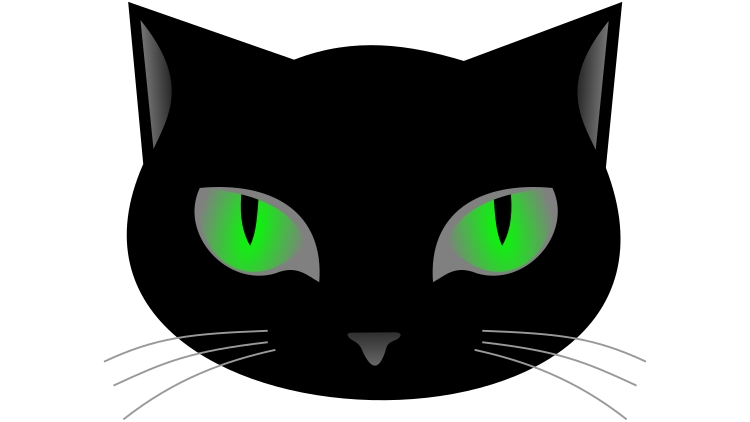
\includegraphics[width=1.2\textwidth, height=0.40\textheight]{figures/logo_picat_alex.jpg}
\end{center}
\end{figure}
\end{minipage}
\end{frame}
%%%%%%%%%%%%%%%%%%%%%%%%%%



\begin{frame}[fragile]

    \frametitle{Listas}

   \begin{block}{}
     \begin{itemize}
      \item Requisito: conceito de recursividade, \textit{aterramento} etc,  dominados!
      
      \pause
      \item  Os conceitos são os próximos os das  LPs convencionais
           \pause 
     \item Essencialmente vamos computar sob uma árvore
         binária (\textcolor{green}{cada nó sempre tem duas ramificações})

           \pause 
      \item Lembrando que uma estrutura binária de árvore tem uma
      equivalência com uma árvore n-ária (ver livro de Estrutura de Dados)

           \pause 
       \item Logo,  listas são estruturas flexíveis e poderosas!

    \end{itemize}
    
    \end{block}
    
\end{frame}





\begin{frame}
 % \frametitle{Fluxo do Cálculo Recursivo}
\frametitle{Ilustrando uma Lista em Formato Binário}

\begin{figure}[!htb]
\centering
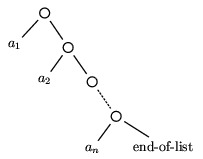
\includegraphics[width=.7\textwidth, height=0.650\textheight]{figures/ilustra-lista-01.jpg}
%\label{fig_ilustra_arv}
\caption{Uma estrutura  Lista -- Homogênea}
\end{figure}

\end{frame}


\begin{frame}
  \frametitle{Ilustrando  Listas e o Operador `\textbf{|}' (ou `\textbf{:}' da figura)}
\begin{figure}[!htb]
\centering
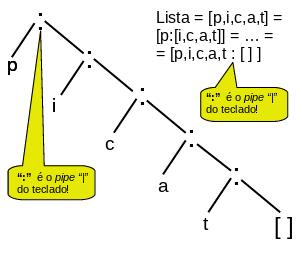
\includegraphics[width=.7\textwidth, height=0.650\textheight]{figures/lista-picat-01.jpg}
%\label{fig_arv_recurs_2}
\caption{Listas são inerentemente \textbf{recursivas}!}
\end{figure}
\end{frame}



\begin{frame}
 \frametitle{Exemplos de Listas}
\begin{figure}[!htb]
\centering
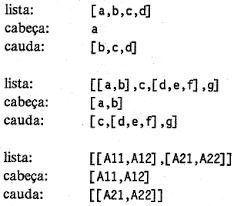
\includegraphics[width=.7\textwidth, height=0.650\textheight]{figures/exemplo_listas_01.jpg}
%\label{fig_arv_recurs_2}
%\caption{Fluxo Recursivo 2}
\end{figure}
\end{frame}



%%%%%%%%%%%%%%%%%%%%%%%%%%%%%%%%%%%%%%%%%%%%%%%%%%%%
\begin{frame}[fragile, allowframebreaks=0.9]
 \frametitle{Sintaxe das Listas}


\begin{block}{Definições iniciais (e recursivas)}
\begin{itemize}


\item Uma lista é uma sequência de termos (objetos)

\pause
\item Uma lista é uma estrutura de dados que representa
uma coleção de termos homogêneos

\item Como Picat a tipagem é dinâmica, o tipo só interessa quando
alguma ação é feita sobre ele, as listas em Picat podem
ser heterogêneas

\item Uma lista  apresenta uma hierarquia natural, internamente,
em \textcolor{magenta}{\textbf{cabeça}} de lista e sub-lista, até o fim da lista.

\end{itemize}
\end{block}
%\lbrack       left bracket [
%\rbrack       right bracket ]

\framebreak
\begin{block}{Notação:}
\begin{itemize}
   \item O símbolo ``\lbrack'' é usado para descrever o início de uma lista,
e ``\rbrack'' para o final da mesma;

   \item Exemplo: seja a lista \lbrack a, b, c, d \rbrack,  logo um predicado cujo
argumento seja algumas letras,  tem-se uma lista do tipo:\\
  \begin{itemize}
  \item letras(\lbrack  a, b, c, d \rbrack )
 \item Onde `a' é  o   \textit{cabeça} (primeiro elemento) da lista
 \item e \lbrack b, c, d \rbrack é uma \textit{sub-lista} que é uma lista!
  \end{itemize}

\item Os elementos de uma lista são lidos da esquerda para direita;

\item  A ``{\em sub-lista}'' \lbrack b,  c, d \rbrack é conhecida como  \textcolor{magenta}{resto} ou
\/ ``\textcolor{magenta}{{\em cauda}}'' da lista;
        
\item   Esta sub-lista é uma lista e toda definição segue-se recursivamente.
 \end{itemize} 

\end{block}


\framebreak
\begin{block}{Operador ``{\bf |}'':}

\begin{itemize}
  \item ``{\em  Como vamos distinguir de onde se encontra
a cabeça  da cauda da lista?}'' 

  \item Com as listas novos símbolos foram introduzidos, 
isto é, além dos delimitadores \lbrack \ldots \rbrack, há um 
 novo operador que \textbf{separa} 
 ou \textbf{define} quem é a elemento cabeça da lista e  cauda. 

  \item Este operador é conhecido como
 ``{\em pipe}'' (ou \textit{barra vertical}), simbolizado por ``{\bf |}'', que 
 separa  o lado esquerdo  da direita da lista. 
 
  \item  Esta separação  é necessário para se realizar os 
  \textit{casamentos de padrões} nas linguagens lógicas.

\end{itemize}
\end{block}

\framebreak
\begin{block}{Exemplos de \textcolor{magenta}{{\em \textbf{casamentos}}}:}

\begin{footnotesize}
\begin{verbatim}
 [ a, b, c, d ] = X
 [ X | b, c, d ]  =  [ a, b, c, d ]
 [ a | b, c, d ]  =  [ a, b, c, d ]
 [ a , b | c, d ]  =  [ a, b, c, d ]
 [ a , b , c | d ]  =  [ a, b, c, d ]
 [ a , b , c , d | [] ]  =  [ a, b, c, d ]
 [] = X
 [ [ a | b , c , d] ] = [ [ a , b , c , d ] ]
 [  a | b , c , [ d ] ] = [  a , b , c , [ d ] ]
 [  _ | b , c , [d ] ] = [  a , b , c , [ d ] ]
 [  a | Y ] = [  a , b , c ,  d ]
 [  a | _ ] = [  a , b , c ,  d ]
 [  a , b | c , d ] = [  X , Y | Z ]
 \end{verbatim}
\end{footnotesize}
\end{block}

\framebreak
\begin{block}{Contra-exemplos de \textcolor{magenta}{{\em \textbf{casamentos}}}:}

\begin{verbatim}
 [ a , b | [c, d] ]  !=  [ a, b, c, d ]
 [ [ a , b , c , d] ]  !=  [ a, b, c, d ]
 [  a , b , [ c ] , d, e ]  !=  [ a, b, c, d, e ]
 [ [ [ a ] | b , c , d] ] != [ [ a , b , c , d] ]
 \end{verbatim}

\end{block}

\framebreak
\begin{itemize}
  \item Estes  casamentos de termos de uma lista
  são também conhecidos  por \textcolor{magenta}{{\em matching}} 

\item  Devido ao fato de listas modelarem
qualquer estrutura de dados, invariavelmente, seu uso  é extensivo
há  problemas em geral (dos simples a complexos)

\item Porém, alguns cuidados no uso de predicados com \textcolor{magenta}{\textit{backtracking}}.
 Acompanhe os exemplos.

\item Os próximos exemplos encontram-se no arquivo: \textcolor{red}{\textbf{\url{../picat/listas.pi}}}

\end{itemize}


\end{frame}
%%%%%%%%%%%%%%%%%%%%%%

\begin{frame}[fragile]

\frametitle{Exemplos sobre Listas (e Implementações)}

\begin{enumerate}
  \item Comprimento de uma lista: retorna um valor numérico
  
  \pause
  \item Se um elemento $x$ pertence a lista: retorna um valor binário (\textit{true} ou \textit{false})


  \pause
  \item Adicionar um elemento $x$ em uma lista: retorna uma nova lista, o $x$ inserido nesta lista,
  se $x$ já estiver presente, não insira. Em resumo: insere $x$ em $L$ sem repetição.

  \pause
  \item Concatena duas listas: retorna uma terceira lista
  
\end{enumerate}

Em resumo: 4 métodos clássicos!

\end{frame}
%%%%%%%%%%%%%%%%%%%%%%

\begin{frame}[fragile, allowframebreaks=0.9]
\frametitle{Exemplo 01: encontrar o comprimento de uma lista}
 
\begin{itemize}
   \item O comprimento de uma lista é o comprimento de sua \textbf{sub-lista}, mais \textbf{um}
   \item O comprimento de uma lista vazia (\lbrack  \rbrack) é zero.
 \end{itemize} 
 
Em Picat, sob uma \underline{visão funcional}, este enunciado é escrito por:

\begin{verbatim}
comprimento_02( [ ] ) = 0.
comprimento_02([ _ | L ]) = N  => 
             N = 1 + comprimento_02( L ).
\end{verbatim}

\framebreak

Em Picat, sob uma \underline{visão lógica}, este predicado 
pode ser construído como:

\begin{verbatim}
comprimento_01([],N) ?=> N = 0. 
%%% em PROLOG, apenas comprimento_01([],0). PORQUÊ?
comprimento_01([_|L],N)  => 
             comprimento_01( L , Parcial ), 
             N = 1 + Parcial.
\end{verbatim}

\framebreak
Um {\em mapa de memória} é dado por:

\begin{center}
\begin{tabular}[c]{|c|c|c|c|c|c|}
\hline
& Regra & X & T & N & N = N+1\\\hline
compto([a,b,c,d],N) & \#2 & a & [b,c,d] & 3 $\rightarrow$ & 3+1$=$4\\\hline
compto([b,c,d],N) & \#2 & b & [c,d] & 2 $\rightarrow$ & $\nwarrow$ 2+1\\\hline
compto([c,d],N) & \#2 & c & [d] & 1 $\rightarrow$ & $\nwarrow$ 1+1\\\hline
compto([d],N) & \#2 & d & [] & 0 $\rightarrow$ & $\nwarrow$ 0+1\\\hline
compto([],N) & \#1 & -- & -- & -- & $\nwarrow$ 0\\\hline
\end{tabular}
\end{center}
 
 \end{frame}
%%%%%%%%%%%%%%%%%%%%%%%%%%%%%%%%%%%%%%%%%%%%%%%%%%%%%%%%%%%%%%%%%%%%

\begin{frame}[fragile, allowframebreaks=0.9]
\frametitle{Exemplo 02: verificar a pertinência de um objeto na lista}

\begin{itemize}
  \item Verifica se um dado objeto pertence há uma  lista
  \item Um método clássico -- muito usado
  \item Tem embutido no Picat: o \textit{menber}
\end{itemize}

Em Picat, sob uma \underline{visão funcional}, esta função é escrita por:

 \begin{verbatim}
pertence_02( _ , [ ]) = false. 
pertence_02( A, [A|_]) = true. 
% CUIDAR ... em funcoes nao hah ? em ?=> ... 
% sem backtracking em funcoes
pertence_02(A, [B|L]) = X => 
             A != B,
             X = pertence_02(A,L).
\end{verbatim}

%O interessante é observar a versatilidade 
%deste  predicado em várias situações:


\framebreak
Em Picat, sob uma \underline{visão lógica}, este predicado 
pode ser construído como:
\begin{verbatim}
pertence_01( A, [A|_]) ?=> true. 
% Again, backtracking CONTROLADO ... diferente do Prolog
pertence_01(A,[B|L])  => 
             A != B ,
             pertence_01(A,L).
\end{verbatim}

\end{frame}


\begin{frame}[fragile, allowframebreaks=0.9]
\frametitle{Exemplo 03: adicionar um elemento  em uma lista}

\begin{itemize}
  \item Um objeto é adicionado no início da lista (sem repeti\c{c}ão) caso este já
 esteja contido na lista, a lista original é a retornada:
%  \item 
\end{itemize}

Em Picat, sob uma \underline{visão funcional}, esta função é escrita por:
 
\begin{verbatim}
add_X_lista_02(X, [ ]) = [X]. 
add_X_lista_02(X, Y) = Z =>
          pertence_02(X, Y) = true,
          Z = Y ;
          Z = [ X | Y ].
\end{verbatim}


\framebreak
Em Picat, sob uma \underline{visão lógica}, este predicado 
pode ser construído como:
\begin{verbatim}

add_X_lista_01(X, [ ], Z )  ?=> Z = [X]. 
add_X_lista_01(X, Y, Z) ?=>
          pertence_01(X, Y),
          Z = Y .
add_X_lista_01(X, Y, Z) =>
          Z = [ X | Y ].

\end{verbatim}

\end{frame}




\begin{frame}[fragile, allowframebreaks=0.9]
\frametitle{Exemplo 04: união de duas listas}

\begin{itemize}
  \item O método de  união ou concatenação entre duas listas,
 resultando em uma terceira lista

 \item Este predicado é conhecido como \textit{append} ou \textit{concatena}. O \textit{append} está 
pronto na  biblioteca default do Picat

\item Há uma versão simplificada: \texttt{L3 = L1 \textbf{++} L2}

\end{itemize}

Em Picat, sob uma \underline{visão funcional}, esta função é escrita por:
\begin{verbatim}
uniao_02( [], X ) = X. 
uniao_02( [X|L1], L2 ) = L3 => 
                           L3 = [X | uniao_02( L1, L2 )].
\end{verbatim}

\framebreak

Em Picat, sob uma \underline{visão lógica}, este predicado 
pode ser construído como:

\begin{verbatim}
uniao_01( [] , X, Y ) ?=> Y = X. 
uniao_01( A , L2, R  ) =>  A = [X|L1] , 
                           R = [X|L3] , 
                           uniao_01( L1, L2, L3 ).
\end{verbatim}

\end{frame}


\begin{frame}[fragile]

\frametitle{Geração de  Listas -- \textit{list comprehension}}

\begin{block}{}
\begin{itemize}
  \item O conceito de \textit{list comprehension} veio da programação funcional
  \item Basicamente serve para criarmos ou gerarmos listas
  \pause
  \item Bastante útil e pode ser usada em qualquer parte de um código
  
\end{itemize}
\end{block}

\end{frame}


\begin{frame}[fragile]

\frametitle{Geração de  Listas -- \textit{list comprehension}}

Um \textit{list comprehension} tem o seguinte formato
na criação de listas:
\begin{tabbing}
aa \= aaa \= aaa \= aaa \= aaa \= aaa \= aaa \kill
\> \> \texttt{[$T$ : $E_1$ \texttt{in} $D_1$, $Cond_1$, $\ldots$, $E_n$ in $D_n$, $Cond_n$]} 
\end{tabbing}
\begin{itemize}
  \item $T$ é uma termo (uma expressão num caso genérico)
  \item $E_i$ é um padrão de iteração 
  \item $D_i$ é uma expressão de um valor composto, em geral um intervalo de domínio
  \item Opcionalmente,  condições $Cond_1$,$\ldots$,$Cond_n$  são chamados de \textit{termos}
  \item Esta geração de lista tem a seguinte interpretação: 
  \textit{toda tupla de valores $E_1 \in D_1$, $\ldots$, $E_n \in D_n$, 
  se as condições $Cond_i$ forem verdades, então o valor do termo $T$ 
  é adicionado na lista em construção}
\end{itemize}
\end{frame}


\begin{frame}[fragile]

\frametitle{Geração de  Listas -- \textit{list comprehension}}

Um vetor ou matrizes também pode 
ser construídos com um  \textit{array comprehension} e tem
o seguinte formato:
\begin{center}
\texttt{\{$T$ : $E_1$ \texttt{in} $D_1$, $Cond_1$, $\ldots$, $E_n$ in $D_n$, $Cond_n$\}} 
\end{center}

\pause
Isto é o mesmo como
%It is the same as:
\begin{center}
\texttt{to\_array([$T$ : $E_1$ \texttt{in} $D_1$, $Cond_1$, $\ldots$, $E_n$ in $D_n$, $Cond_n$])} 

\end{center}
\end{frame}


\begin{frame}[fragile]

\frametitle{Exemplos de \textit{list comprehension}}
\begin{footnotesize}
\begin{verbatim}
main => Status = command("clear") ,
		printf("====================================== %d", Status),
    L0 = [I :  I in 10..20],
    L1 = [I :  I in 10..2..20],
    L2 = [I :  I in 1..20, I>10, I<20],
    L3 = [(A,I) : A in [a,b], I in 1..10, I mod 2 == 0],
    L4 = [(I,J,K) :  I in 1..2, J in 3..7, K in 1..10, I+J < K],
    printf("\n L0 : %w " , L0),
    printf("\n L1 : %w " , L1),
    printf("\n L2 : %w " , L2),
    printf("\n L3 : %w " , L3),
    printf("\n L4 : %w " , L4),
    printf("\n FIM\n").
    
%  $ picat geracao_listas.pi    
\end{verbatim}
\end{footnotesize}
\end{frame}



\begin{frame}[fragile]

\frametitle{Saída: \textit{list comprehension}}

\begin{footnotesize}
\begin{verbatim}
====================================== 0
 L0 : [10,11,12,13,14,15,16,17,18,19,20] 
 L1 : [10,12,14,16,18,20] 
 L2 : [11,12,13,14,15,16,17,18,19] 
 L3 : [(a,2),(a,4),(a,6),(a,8),(a,10),(b,2),(b,4),(b,6),(b,8),(b,10)] 
 L4 : [(1,3,5),(1,3,6),(1,3,7),(1,3,8),(1,3,9),(1,3,10),(1,4,6),
 (1,4,7),(1,4,8),(1,4,9),(1,4,10),(1,5,7),(1,5,8),(1,5,9),(1,5,10),(1,6,8),
 (1,6,9),(1,6,10),(1,7,9),(1,7,10),(2,3,6),(2,3,7),(2,3,8),(2,3,9),(2,3,10),
 (2,4,7),(2,4,8),(2,4,9),(2,4,10),(2,5,8),(2,5,9),(2,5,10),
 (2,6,9),(2,6,10),(2,7,10)] 
 FIM
\end{verbatim}
\end{footnotesize}

\textcolor{red}{L4 ... \textit{cortada}}
\end{frame}



%%%%%%%%%%%%%

\begin{frame}[fragile]
\frametitle{Concluindo Listas}

\begin{block}{}
\begin{itemize}
  \item Há muitos predicados e funções prontas sobre listas nos módulos do Picat
  \pause
  \item Contudo, se aprende sobre listas, fazendo \textcolor{magenta}{\textbf{muitos}} métodos
    \pause
  \item A recursividade em sua modelagem, define a \textcolor{magenta}{metodologia de se \textit{programar em lógica}}
    \pause
  \item Exercitar-se para aprender os detalhes!
    \pause
  \item Usar as listas como estrutura base em problemas complexos
  
     \pause
  \item Próxima na aula: buscas (\textcolor{magenta}{\textbf{uso extensivo de listas}})
  
\end{itemize}

\end{block}

\end{frame}
 % cap 4 nesse capitulo falar mais de listas

\section{Buscas}


%%%%%%%%%%%%%%%%%%%%%%%%%%
\begin{frame}
\frametitle{Buscas}
\begin{minipage}{0.47\textwidth}
    \begin{itemize}
        \item O que é uma \textit{busca}?
        \item Problemas $\Rightarrow$ buscar ...
        \item Buscas em estruturas quaisquer
        \item Listas são o suficiente!
        \item Núcleo das buscas
        \item Exemplo
    \end{itemize}
\end{minipage}
\begin{minipage}{0.5\textwidth}
\begin{figure}[ht!]
\begin{center}
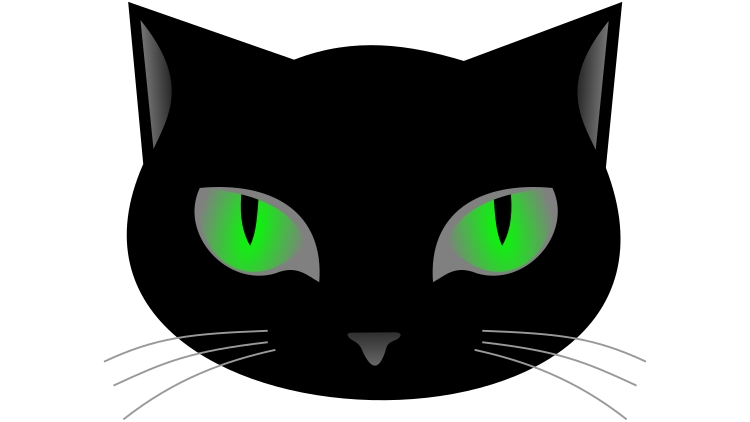
\includegraphics[width=1.2\textwidth, height=0.40\textheight]{figures/logo_picat_alex.jpg}
\end{center}
\end{figure}
\end{minipage}
\end{frame}
%%%%%%%%%%%%%%%%%%%%%%%%%%




\begin{frame}

    \frametitle{Buscas}

   \begin{block}{}
     \begin{itemize}
      \item Requisito: conceitos de listas e recursividade  dominados!
       \pause
      \item Além destes: noções sobre grafos, árvores, nós, etc

       \pause
      \item Solucionar problemas implicar em percorrer estados (um caminho)
      que levem há um estado--solução      
      
       \pause
      \item Grosseiramente: \textbf{\textcolor{magenta}{estados de problemas $\Leftrightarrow$ estruturas abstratas}}
         
       \pause
      \item Pois, problemas em geral
      se apresentam como uma conexão complexa tipo um \textit{grafo},
      e a varredura sob este grafo é sistemática
      sob uma \textit{árvore de busca}
      \pause
      
     \item Então, computar listas em Picat é uma estratégia
     de resolver problemas!

    \end{itemize}
    
    \end{block}
    
\end{frame}



\begin{frame}[fragile, allowframebreaks=0.9]
  \frametitle{Ciclo Euleriano}

\begin{figure}[!htb]
\centering
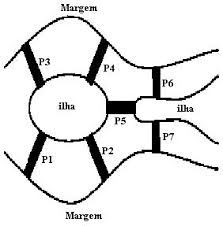
\includegraphics[width=0.560\textwidth, height=0.50\textheight]{figures/ilhas_euler.jpeg}
%%%prolog/scale=0.47
%\label{fig_nos_estados}
\caption{Ciclo Euleriano -- Problema das Pontes de Königsberg}
\end{figure}


\framebreak

\begin{itemize}
  \item No século 18 havia na cidade de Königsberg (antiga Prússia)  um conjunto de sete pontes
 (identificadas pelas letras de P1 até P7 na figura ao lado ) que cruzavam o rio  Prególia. 
 Elas conectavam duas ilhas  entre si e as ilhas com as margens esquerda
 e direita.
 
\item Os habitantes daquela cidade perguntavam-se se era possível cruzar 
as sete pontes numa caminhada contínua sem que se passasse duas vezes por 
qualquer uma das pontes.

\item  Embora intrigante, este problema foi atacado por Leonard Euler (1736) e demonstrou
que isto não era possível para um grafo qualquer

\item Curiosamente, este problema é \underline{\textit{fácil}} de resolver. Euler demonstrou
uma relação entre vértices e arestas para que isto fosse possível.
\end{itemize}

\end{frame}



\begin{frame}[fragile, allowframebreaks=0.9]
 \frametitle{Caminho Hamiltoniano}


\begin{figure}[!htb]
\centering
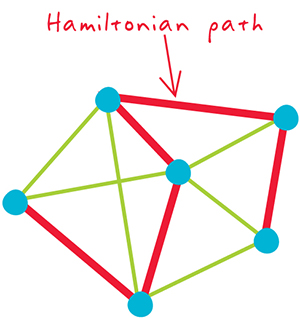
\includegraphics[width=.6\textwidth, height=0.60\textheight]{figures/hamiltonian_path.jpg}
%%%prolog/scale=0.47
%\label{fig_nos_estados}
\caption{Caminho Hamiltoniano -- Há um caminho que passe por todas cidades uma única vez?}
\end{figure}


\framebreak

\begin{itemize}
  \item \textcolor{magenta}{\textbf{Diferente}} do ciclo Euleriano, o caminho Hamiltoniano, \textcolor{magenta}{origem
  e destino são diferentes}
 
\item Todos os nós precisam ser visitados uma única vez sem repetição

\item  Num grafo pode haver muitos caminhos  Hamiltonianos, mas, pode
       não existir nenhum!

\item Ao contrário do ciclo Euleriano, este problema, computacionalmente é \underline{\textit{difícil}} de resolver!

\item Vamos usar o caminho Hamiltoniano como exemplo, para construir um algoritmo  ingênuo, mas que funciona bem!
\end{itemize}

\end{frame}


\begin{frame}[fragile,  allowframebreaks=0.8]
\frametitle{Problemas, Estados, Grafos e  Árvores de Buscas}

Contextualizando estes termos:

\begin{itemize}

  \item Em geral, problemas podem ser vistos como \textit{fotografias 
  instantâneas} de uma situação, isto é, \textcolor{magenta}{\textbf{um estado discreto}}
   
  \item Uma \textit{sucessão} destes estados, compõem \textit{um caminho} de um estado $i$ ao estado $j$
  
  \item Assim, estes \textit{estados} são representados pelos \textit{nós dos grafos}, e a ligação entre 
  estes, são resultados de \textit{uma ação}, mudança ou evolução do problema
  
  \item Há um estado particular chamado \textit{inicial},  vários outros de estados \textit{intermediários},
   e outros estados \textit{finais}
  
  \item Se o problema tiver várias soluções,  o mesmo apresenta vários caminhos do estado inicial ao  final.
  
  \item Assim uma sucessão ou transição válida entre estados, é conhecido como uma \textit{solução} ou \textit{prova}
     do problema

  \item Essencialmente vamos varrer uma estrutura
     entre estados ou nós, de modo sistemático até encontrarmos
     uma solução aceitável/desejável.

    \item Logo, vamos empregar alguns conceitos da teoria dos grafos, em modelar problemas e resolvê-los 
  por um esquema de busca computacional
  
    
\end{itemize}

\end{frame}


%%%%%%%%%%%%%%


\begin{frame}[fragile]
\frametitle{Problema do Robô no Labirinto}

\begin{figure}[!htb]
\centering
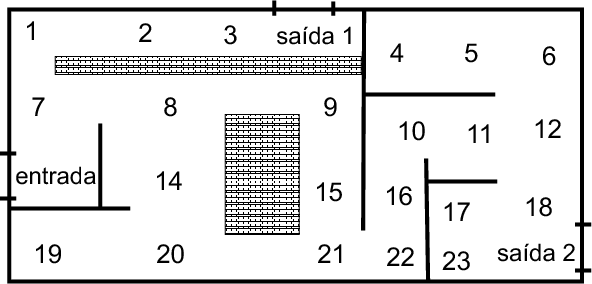
\includegraphics[width=.79\textwidth, height=0.45\textheight]{figures/labirinto_robo.png}
%%%prolog/scale=0.47
%\label{fig_nos_estados}
%\caption{Google ...}
\end{figure}

\textcolor{magenta}{Imagine qualquer problema: uma busca na WEB,
atomicidade de transações de BD, máquina de café, carro autônomo, etc }

\end{frame}



\begin{frame}[fragile]
\frametitle{Problemas de Grafos se Transformam em Árvores de Buscas}

\begin{figure}[!htb]
\centering
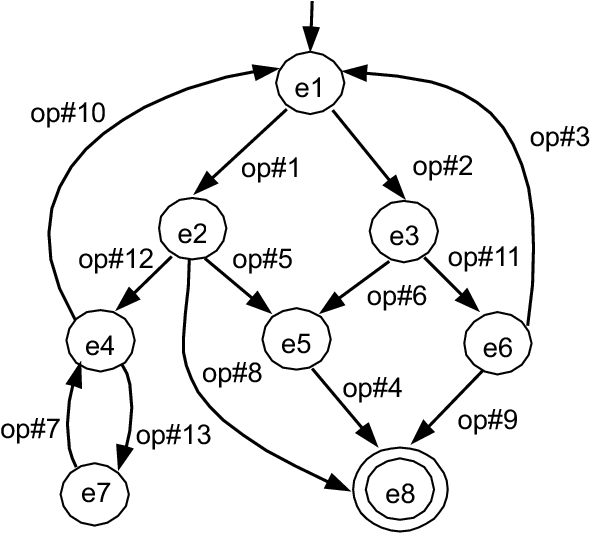
\includegraphics[width=0.6\textwidth, height=0.55\textheight]{figures/arv_buscas_estados.png}
\end{figure}

\textcolor{magenta}{Resumindo, os problemas são modelados  em 
estruturas  complexas, tais como grafos, mas o processo de solução
se mantém: \textbf{realizar uma busca, tal como uma estrutura de uma árvore (listas)} !}

\end{frame}



\begin{frame}[fragile]
\frametitle{Problemas de Grafos se Transformam em Árvores de Buscas}


\begin{figure}[!htb]
\centering
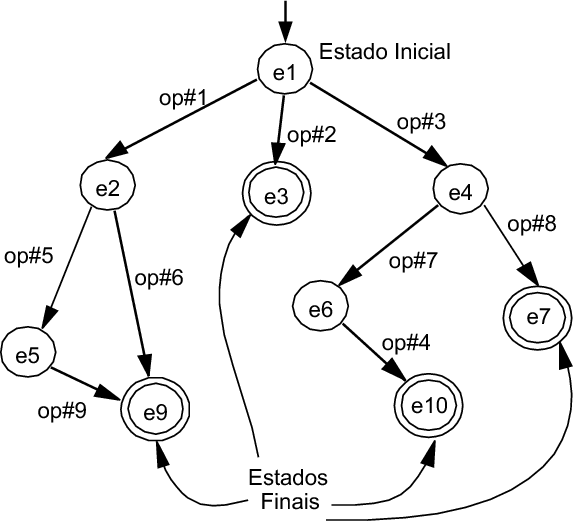
\includegraphics[width=0.7\textwidth, height=0.55\textheight]{figures/arv_buscas_finais.png}
\end{figure}

% \begin{minipage}{0.5\textwidth}
% \begin{figure}[ht!]
% \begin{center}
% 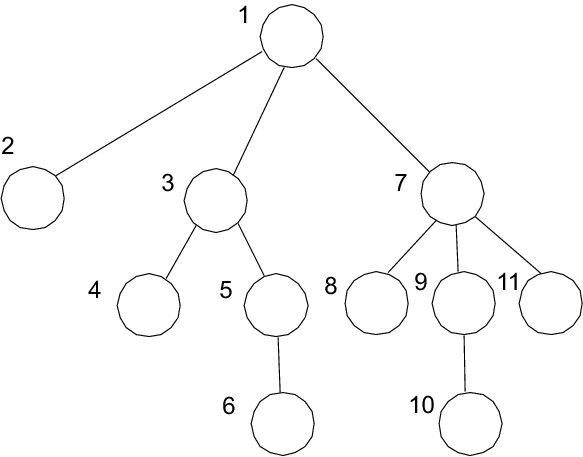
\includegraphics[width=0.7\textwidth, height=0.30\textheight]{figures/busca_grafo.png}
% \end{center}
% \end{figure}
% \end{minipage}
% \end{frame}
%
\begin{center}
\textcolor{magenta}{Assim, a idéia é percorrer os \textbf{ramos destas  árvores}, de maneira
sistemática. Um \textbf{caminho} da raiz há um nó terminal de interesse, este é uma solução do
problema. Logo, tudo se resume em manipular muitas \textbf{listas}!}
\end{center}

\end{frame}


\begin{frame}[fragile, allowframebreaks=0.9]
  \frametitle{Núcleo Geral de Buscas}

\textcolor{red}{Pseudo-código já em Picat}

\begin{verbatim}
resolve(P) =>
      inicio(Start),
      busca(Start,[Start],Qsol),
      imprime_saida(Qsol,P).

busca(S,P,P) ?=>  objetivo(S).    % objetivo alcancado : FIM    
busca(S,Visited,P) =>
     proximo_estado(S,Nxt),       % gera um proximo estado  
     estado_seguro(Nxt),          % verifica se este estado é válido 
     sem_loop(Nxt,Visited),       % verifica se está em loop .. repete estados 
     busca(Nxt,[Nxt|Visited],P).  % continue a busca recursiva 
\end{verbatim}


\framebreak


\begin{verbatim}

sem_loop(Nxt,Visited) :-
      \+member(Nxt,Visited).

proximo_estado(S,Nxt) =>   < fill in here >.
estado_seguro(Nxt) =>     < fill in here >.
sem_loop(Nxt,Visited) =>  < fill in here >.     
                       
inicio(...).
objetivo(...).

\end{verbatim}


\textcolor{red}{Vamos reescrever este pseudo-código em um problema!}


\end{frame}


\begin{frame}[fragile]
\frametitle{Caminho Hamiltoniano Aplicado}

\begin{figure}[!htb]
\centering
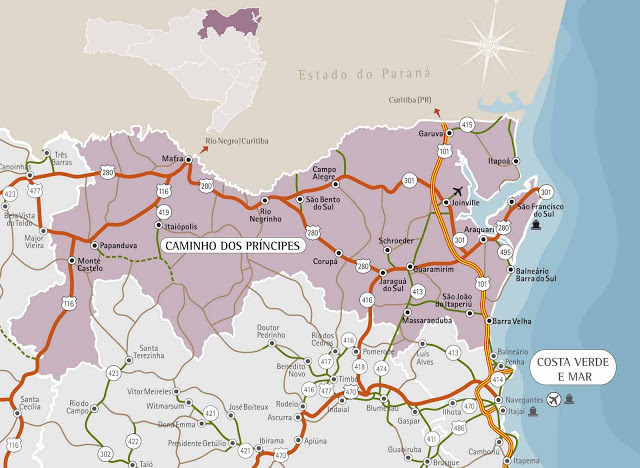
\includegraphics[width=.8\textwidth, height=0.567\textheight]{figures/mapa-norte-santa-catarina.jpg}
%%%prolog/scale=0.47
%\label{fig_nos_estados}
%\caption{Mapa do norte de Santa Catarina}
\end{figure}

Seja um viajante que sai cedo de Joinville, e chegar a noite
em Blumenau, passando por algumas destas cidades uma única vez!

\end{frame}


\begin{frame}[fragile]
\frametitle{Cidades Escolhidas pelo Viajante}

\begin{figure}[!htb]
\centering
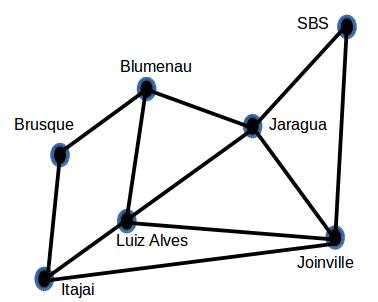
\includegraphics[width=.8\textwidth, height=0.567\textheight]{figures/mapa01SC.jpg}
%%%prolog/scale=0.47
%\label{fig_nos_estados}
%\caption{Mapa do norte de Santa Catarina}
\end{figure}

\end{frame}




\begin{frame}[fragile, allowframebreaks=0.9]

\frametitle{Modelagem do Problema -- \textit{O nosso viajante do Vale do Itajaí}}

\begin{itemize}
  \item Em nosso problema temos 7 cidades pré-escolhidas

  \item A lista de cidades são:
\begin{footnotesize}
 \begin{verbatim}
index(-) %% lista de todas cidade do mapa
as_cidades( [ brusque, blumenau, itajai, luiz_alves,
            jaragua, sao_bento, joinville ] ).
\end{verbatim}
 \end{footnotesize}

\item  Duas cidades em particular:
\begin{footnotesize}
\begin{verbatim}
index(-)
destino( blumenau ).

index(-)
origem( joinville ).
\end{verbatim}  
\end{footnotesize}
  
\item As estradas transitáveis entre as cidades definem
  o nosso mapa, consequentemente um grafo entre
  cidades:
\begin{footnotesize}
\begin{verbatim}
%% MAPA da região
index(-,-)
arco(joinville, sao_bento)  .
arco(joinville, itajai)     .
arco(joinville, jaragua)     .
arco(joinville, luiz_alves)     .
arco(jaragua, sao_bento)    .
arco(jaragua, blumenau)     .
arco(jaragua, luiz_alves)   .
arco(itajai, luiz_alves)    . 
arco(blumenau, luiz_alves)    . 
arco(blumenau, itajai)      .
arco(brusque, itajai)       .
arco(brusque, blumenau)     .
\end{verbatim} 
\end{footnotesize}  

\item As estradas entre as cidades são bidirecionais. Se  há estrada para ir
da cidade $X$ a cidade $Y$ então na outra direção é verdadeiro.
Em regras isto é escrito por:
\begin{footnotesize}
\begin{verbatim}
/* BI-DIRECIONALIDADE DOS ARCOS */
move_no(X,Y) ?=> arco(X,Y).
move_no(X,Y)  => arco(Y,X).
\end{verbatim} 
\end{footnotesize}  

\item Claro, este problema é pequeno e construindo o grafo dá para constatar que existe
mais uma solução para o nosso viajante

  \item Para resolver este problema vamos utilizar uma \textbf{\textcolor{magenta}{busca em profundidade}}
  
  \item Esta \textbf{\textcolor{magenta}{busca em profundidade}}  (do inglês. \textit{depth first search -- DFS}), 
  encontra-se inserida no contexto \textit{buscas em geral},
  visto anteriormente.
\end{itemize}


\end{frame}

\begin{frame}[fragile]
 \frametitle{O \textit{Miolo} ou Núcleo  da Busca}

\begin{footnotesize}
\begin{verbatim}
busca_DFS ( [ No_corrente | Caminho] , L_sol) ?=>
      destino(No_final),       %%% condicao de parada 1
      No_corrente == No_final,
      L_sol = [ No_corrente | Caminho ],
      as_cidades(L_Todas_Cidades),    %%% condicao de parada 2
      %% TODAS CIDADES FORAM VISITADAS
      length (L_sol) ==  length(L_Todas_Cidades),
      write(L_sol),
      printf(" \n UMA SOLUCAO ....: OK\n ==>"). 

busca_DFS (  [NoH | Caminho], Solucao) =>
      %%% explorar um novo movimento ou um novo noh
      move_no(NoH , Novo_NoH), 
      %% testar se este novo noh nao foi visitado ainda
      %% ou novo_NOH eh permitido
      not( member(Novo_NoH, [NoH|Caminho]) ),
      busca_DFS(  [Novo_NoH , NoH | Caminho ] , Solucao).
\end{verbatim}
\end{footnotesize}

\end{frame}


\begin{frame}[fragile]
 \frametitle{O Código Completo}

\begin{itemize}
  \item Acompanhar as explicações do código de:\\
\url{https://github.com/claudiosa/CCS/blob/master/picat/hamiltoniano_DFS.pi}

   \item Muitos elementos da linguagem neste código

  \item Confira a execução
\end{itemize}
\end{frame}




\begin{frame}[fragile]
\frametitle{Saída}

\begin{footnotesize}
\begin{verbatim}
$ picat hamiltoniano_DFS.pi 
..............................
[blumenau,brusque,itajai,luiz_alves,jaragua,sao_bento,joinville] 
 UMA SOLUCAO ....: OK
 ==>joinville : sao_bento : jaragua : luiz_alves : itajai : brusque 
 : blumenau : 
 Cidade Inicial: joinville 
 Cidade Final: blumenau
 Total de cidades visitadas: 7
 CPU time 0.000000 em SEGUNDOS 
 OVERALL PICAT CPU time 0.013000 em SEGUNDOS 
 Backtrackings total 0  
 =========================================
 [ccs@gerzat picat]$ 
\end{verbatim}
\end{footnotesize}

\begin{center}
\textcolor{magenta}{Existe uma função chamada \textbf{findall}, cujo valor
de retorno é uma lista com todas soluções possíveis de um dado predicado!}
\end{center}

\end{frame}



\begin{frame}[fragile]
\frametitle{Uma Soluç\~ao}

\begin{figure}[!htb]
\centering
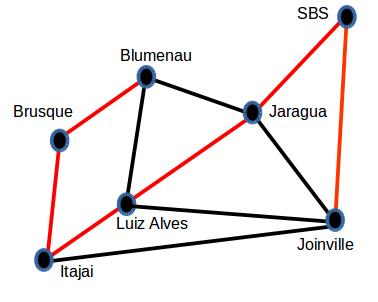
\includegraphics[width=.8\textwidth, height=0.567\textheight]{figures/mapa02SC.jpg}
%%%prolog/scale=0.47
%\label{fig_nos_estados}
%\caption{Mapa do norte de Santa Catarina}
\end{figure}

\end{frame}




\begin{frame}[fragile]
\frametitle{Concluindo Buscas}

\begin{block}{}
\begin{itemize}
  
  
  \item A recursividade na modelagem das buscas, 
  define \textcolor{magenta}{\textbf{uma metodologia}} de
   se \textit{programar em lógica} e resolver problemas
 
 
  \pause
  \item A área de buscas é ampla e apresenta muitas variações. Apresentamos
  nesta seção um \textcolor{magenta}{\textbf{núcleo mágico}}, que pode ser utilizado em muitas outras
  estrategias--métodos de buscas. 
  
  
  \pause
  \item Praticamente todos os métodos de buscas fazem o uso extensivo das 
  \textcolor{magenta}{\textbf{listas}} em problemas complexos
  
  \pause
  \item Aos problemas complexos, há outras técnicas de programação
  para resolvê-los.
    
  \pause
  \item Assunto das próximas seções: \underline{PD}, Planejamento e CP
\end{itemize}

\end{block}

\end{frame}



       
\section{Programação Dinâmica}

%%%%%%%%%%%%%%%%%%%%%%%%%%
\begin{frame}
\frametitle{Programação Dinâmica}
\begin{minipage}{0.47\textwidth}
    \begin{itemize}
        \item O que é a PD?
        \item Características
        \item Importância
        \item Exemplo
        
    \end{itemize}
\end{minipage}
\begin{minipage}{0.5\textwidth}
\begin{figure}[ht!]
\begin{center}
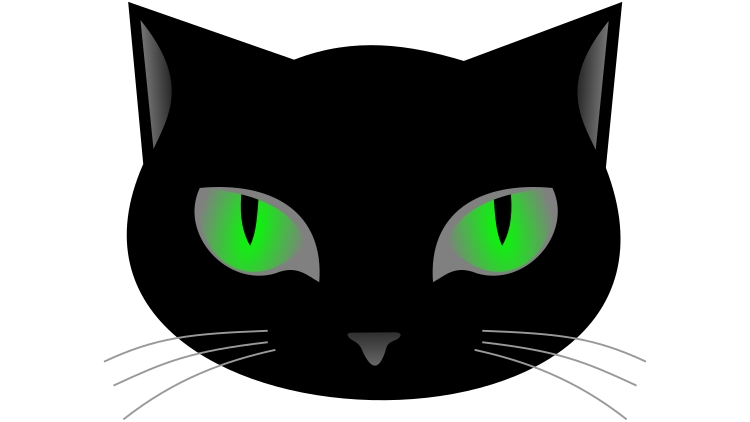
\includegraphics[width=1.2\textwidth, height=0.40\textheight]{figures/logo_picat_alex.jpg}
\end{center}
\end{figure}
\end{minipage}
\end{frame}
%%%%%%%%%%%%%%%%%%%%%%%%%%


\begin{frame}[fragile]
%[fragile, allowframebreaks=0.9]

    \frametitle{Programação Dinâmica (PD) -- I}

   \begin{block}{}
     \begin{itemize}
      \item Uma poderosa \textcolor{magenta}{\textit{técnica de programação}}  que  contorna a complexidade de certos problemas
      exponenciais
      
       \pause
       \item O problema \textbf{deve} apresentar uma \textcolor{magenta}{\textit{\underline{regra de recorrência}}}
       
      \pause
      \item A idéia é que todos os cálculos feitos a partir desta \textit{regra de recorrência},
     sejam armazenados numa \textit{tabela dinâmica} e consultados para reuso de novos cálculos de outras
      instâncias
      
      \pause
      \item Esta \textcolor{magenta}{\textit{técnica de programação}} 
      utiliza uma \textit{tabela dinâmica} nos cálculos intermediários,
      evitando a repetição do que já foi calculado anteriormente, é conhecida como:
      \textcolor{magenta}{Programação Dinâmica}, ou simplesmente:
       \underline{\textcolor{magenta}{\textbf{PD}}}

    \end{itemize}
    
    \end{block}
    
\end{frame}



\begin{frame}[fragile]
\frametitle{Programação Dinâmica (PD) -- II}

\begin{figure}[!htb]
\centering
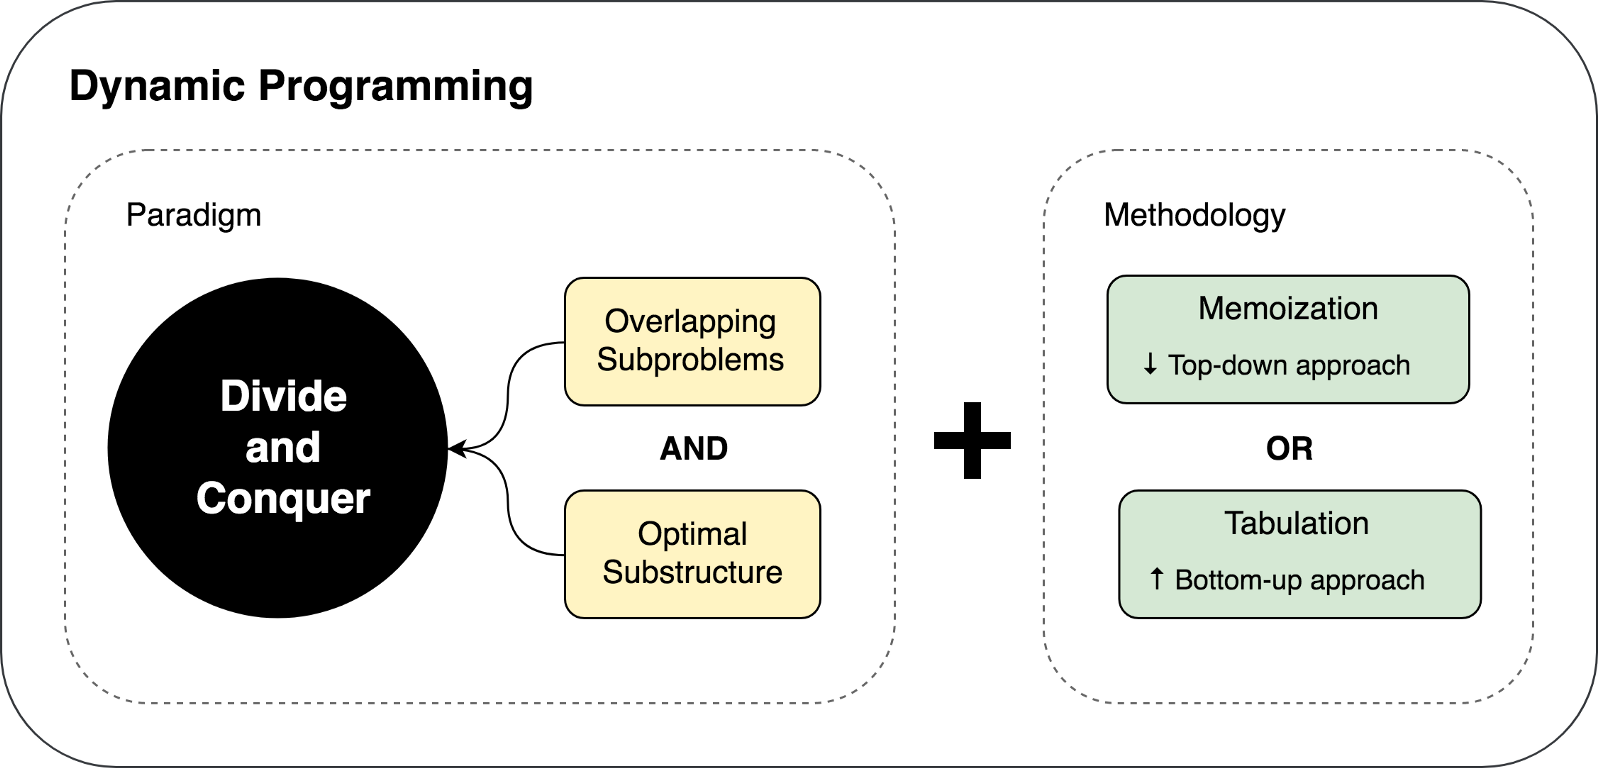
\includegraphics[width=0.95\textwidth, height=0.70\textheight]{figures/ilustra_PD.png}
\caption{Conceitos da Programação Dinâmica -- (PD) -- Resumos}
\end{figure}
\end{frame}






\begin{frame}[fragile]
%[fragile, allowframebreaks=0.9]

    \frametitle{Programação Dinâmica (PD) -- III}

   \begin{block}{}
     \begin{itemize}

      \item Como Picat usa a recursão, na programação em lógica, nada mais
      natural do que esta ter a PD disponível 

       \pause
       \item O comando que cria uma tabela para um determinado predicado é o  \textcolor{magenta}{\textbf{\textit{tabling}}}
 
        \pause
       \item O \textit{tabling}  é um dos elementos fortes do planejador do Picat (módulo \textit{planner})

        \pause
       \item Assim a PD, faz a complexidade ser espacial devido o uso de memória em seus cálculos intermediários

        \pause
       \item O exemplo escolhido para ilustrar a PD em Picat, veio do texto \textit{Modeling and Solving AI
        Problems in Picat}, de Roman Barták e Neng-Fa
    \end{itemize}
    
    \end{block}
    
\end{frame}



\begin{frame}[fragile]
%[fragile, allowframebreaks=0.9]

\frametitle{Exemplo de Uso da Programação Dinâmica -- (PD)}

\begin{itemize}
  \item Seja o binômio ${\left(x + y\right)}^n$, conhecido como \textit{Binômio de Newton}

  \pause 
  \item Casos particulares são:
  \item  ${\left(x + y\right)}^0 = 1$
  \item  ${\left(x + y\right)}^1 = x + y$
  \item  ${\left(x + y\right)}^2 = x^2 + 2xy + y^2$
  
  \pause
  \item  ${\left(x + y\right)}^2 = x^2y^0 + 2x^1y^1 + x^0y^2$
  \item  ${\left(x + y\right)}^3 = x^3y^0 + 3x^2y^1 + 3x^1y^2 + x^0y^3$
  \item  ${\left(x + y\right)}^4 = x^4y^0 + 4x^3y^1 + 6x^2y^2 + 4x^1y^3 + x^0y^4.$
  \item  .......
  \pause
 \item Como obter estes coeficientes  polinômios?  

\end{itemize}
    
\end{frame}


\begin{frame}[fragile]
%[fragile, allowframebreaks=0.9]

\frametitle{Exemplo de Uso da Programação Dinâmica -- (PD)}

\begin{figure}[!htb]
\centering
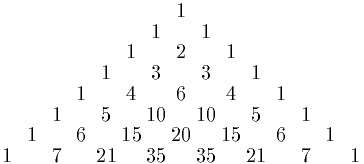
\includegraphics[width=0.70\textwidth, height=0.60\textheight]{figures/pascal_triangle_01.jpg}
%%%prolog/scale=0.47
%\label{fig_nos_estados}
\caption{O triângulo de Pascal}
\end{figure}
\end{frame}


%%%%%%%%%%%%%%%%%%%%%%%%%%%%%%%%%%%%%%%
\begin{frame}[fragile]
%[fragile, allowframebreaks=0.9]

\frametitle{Exemplo de Uso da Programação Dinâmica -- (PD)}

\begin{figure}[!htb]
\centering
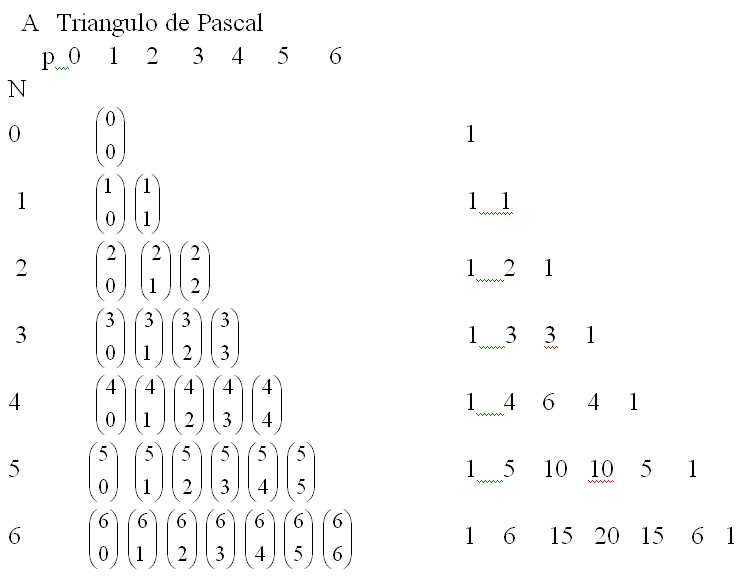
\includegraphics[width=0.850\textwidth, height=0.650\textheight]{figures/pascal_triangle_02.jpg}
%%%prolog/scale=0.47
%\label{fig_nos_estados}
\caption{O triângulo de Pascal -- Coeficientes Binomiais}
\end{figure}
    
\end{frame}

%%%%%%%%%%%%%%%%%%%%%%%%%%%%%%%%%%%%%%%

\begin{frame}[fragile]
%[fragile, allowframebreaks=0.9]

\frametitle{Formulação Matemática -- I}

\begin{itemize}
  \item O \textit{coeficiente binomial}, também chamado de \textit{número binomial}, 
de um número $n$, na classe $k$, consiste no número de combinações de $n$ termos, $k$ a $k$. 

\pause
  \item O número binomial de um número $n$, na classe $k$, pode ser escrito como:

$$ {n \choose k}= \frac {n!}{k!(n-k)!}=\frac {n(n-1)(n-2)\cdots(n-k+1)}{k!}$$
\end{itemize}   
    
\end{frame}



\begin{frame}[fragile]
%[fragile, allowframebreaks=0.9]

\frametitle{Formulação Matemática -- II}

\begin{itemize}
  \item Alternativa ao cálculo do fatorial, tem-se a relação de Stiffel:

 $$ {n\choose k}={n-1\choose k-1}+{n-1\choose k}$$  
    

\pause
  \item  O coeficiente binomial é muito utilizado no Triângulo de Pascal, onde o 
  termo na linha $n$ e coluna $k$ é  dado por: ${n-1 \choose k-1}$
  
  \pause
  \item A fórmula de Stiffel é \textcolor{red}{recorrente} e diretamente escrita em Picat.\\
  Veja os códigos ...
\end{itemize}   
    
\end{frame}


\begin{frame}[fragile] 

\frametitle{Código em Partes}

\begin{footnotesize}
\begin{verbatim}
import datetime.   %%% para o statistics
import util.


table
c(_, 0) = 1.
c(N, N) = 1.
c(N,K) = c(N-1, K-1) + c(N-1, K).
\end{verbatim}
\end{footnotesize}    

\begin{center}
\textcolor{magenta}{Esta fórmula é semelhante com a sequência de Fibonacci, vista
na seção de recursividade, mas aqui temos 2 argumentos em \texttt{c(N,K)}. 
Logo, o número de 
variações de cada coeficiente \texttt{c(N,K)}, 
cresce muito os cálculos repetidos!}
\end{center}

\end{frame}



\begin{frame}[fragile] 
\frametitle{Código em Partes}

\begin{footnotesize}
\begin{verbatim}
main  ?=>  
    statistics(runtime,_), % faz uma marca do 1o. statistics
    N = 10, %% ateh uns 30 ... são números grandes ... fatorial
     foreach(I in 0  .. N)
        foreach(J in 0  ..  I)
             printf("  %d", c(I,J))
           end,
          printf(" \n"),
      end, 
    statistics(runtime, [T_Picat_ON, T_final]),
    T = (T_final) / 1000.0, %%% está em milisegundos
    printf("\n CPU time %f em SEGUNDOS ", T),
    printf("\n OVERALL PICAT CPU time %f em SEGUNDOS ", T_Picat_ON/1000.0),
    printf(" \n =========================================\n ")
    %%% , fail descomente para multiplas solucoes
    .
main => printf("\n Para uma solução .... !!!!" ) .
\end{verbatim}
\end{footnotesize}
    
\end{frame}


\begin{frame}[fragile]
 \frametitle{Código Completo}

\begin{itemize}
  \item Acompanhar as explicações do código de:\\
\url{https://github.com/claudiosa/CCS/blob/master/picat/coeficiente_binomial_PD.pi}

  \item Confira a execuç\~ao
\end{itemize}
\end{frame}
%%%%%%%%%%%%%%%%%%%%%%%%%%%%%%%%%%%%%%%%%%%%%%%%%%%%%%%%%%%%%%%
\begin{frame}[fragile]
%[fragile, allowframebreaks=0.9]

\frametitle{Saída}
\begin{footnotesize}
\begin{verbatim}
[ccs@gerzat picat]$ picat coeficiente_binomial_PD.pi 
  1 
  1  1 
  1  2  1 
  1  3  3  1 
  1  4  6  4  1 
  1  5  10  10  5  1 
  1  6  15  20  15  6  1 
  1  7  21  35  35  21  7  1 
  1  8  28  56  70  56  28  8  1 
  1  9  36  84  126  126  84  36  9  1 
  1  10  45  120  210  252  210  120  45  10  1 

 CPU time 0.000000 em SEGUNDOS 
 OVERALL PICAT CPU time 0.009000 em SEGUNDOS  
 =========================================
\end{verbatim}

\end{footnotesize}    

\end{frame}

%%%%%%%%%%%%%%%%%%%%%%%%%%%%%%%%%%%%%%%%%%%%%%%%%%%%%%%%%%%%%%%
\begin{frame}[fragile]
\frametitle{Reflexões sobre PD}


\begin{itemize}
  \item Há outros métodos para se resolver estes problemas

  \pause
  \item O comando \textit{tabling} é a base do módulo \textit{planner},
  usado para resolver \underline{problemas de planejamento}

  \pause
  \item A PD é uma estratégia de programação bem poderosa
  
  \pause
  \item Assunto das próximas seções:  \underline{Planejamento} e PR

  
\end{itemize}

\end{frame}

%%%%%%%%%%%%%%%%%%%%%%%%%%%%%%%%%%%%%%%%%%%%%%%%%%%%%%%%%%%%%%%
 % cap ??? finalizar aqui
\section{Planejamento}


%%%%%%%%%%%%%%%%%%%%%%%%%%
\begin{frame}
\frametitle{Planejamento}
\begin{minipage}{0.47\textwidth}
    \begin{itemize}
        \item O que é Planejamento?
        \item Importância da área
        \item Muitas definições
        \item Exemplo
    \end{itemize}
\end{minipage}
\begin{minipage}{0.5\textwidth}
\begin{figure}[ht!]
\begin{center}
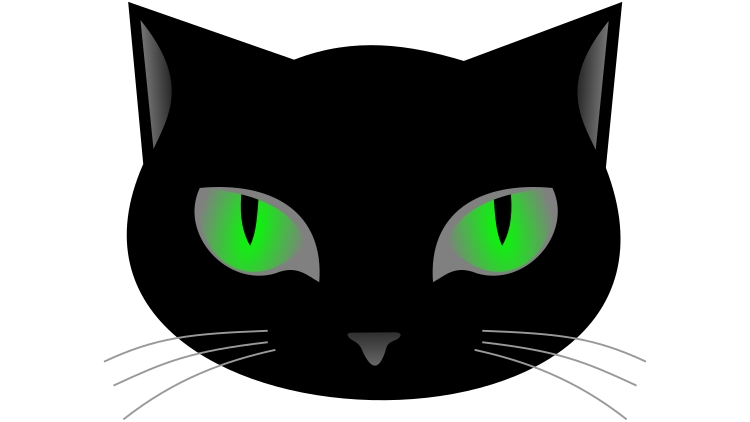
\includegraphics[width=1.2\textwidth, height=0.40\textheight]{figures/logo_picat_alex.jpg}
\end{center}
\end{figure}
\end{minipage}
\end{frame}
%%%%%%%%%%%%%%%%%%%%%%%%%%

\begin{frame}[fragile]
%[fragile, allowframebreaks=0.9]

 \frametitle{Planejamento}

   \begin{block}{}
     \begin{itemize}
      \item Requisitos: recursividade, listas e PD
       \pause
      
      \item Além destes: conceitos grafos, árvores de busca, nós, etc
       
       \pause
      \item \textit{Planejamento} é um \textcolor{magenta}{\textbf{termo amplo e em vários domínios}} 
      
       \pause
      \item \textcolor{red}{O que \textbf{não} é o nosso contexto de \textit{planejamento}?}\\
      Exemplo: planejamento estratégico das empresas, planejar como distribuir
      os dividendos da empresa, orçamento familiar,  etc
      
      \pause
       \item \textcolor{violet}{O que é o nosso contexto de \textit{planejamento}?}
       \pause
       Questões que envolvam um ambiente, um agente (um programa, um robô, etc), sensores,
      e ações que modifiquem estados.\\ Exemplo clássico:  robótica em geral
 
    \end{itemize}
    
    \end{block}
    
\end{frame}



\begin{frame}[fragile]
%[fragile, allowframebreaks=0.9]

    \frametitle{Planejamento}

   \begin{block}{}
     \begin{itemize}
 
       
      \item Problemas em geral necessitam de um \textcolor{magenta}{\textbf{plano}} 
      para serem solucionados, assim,
      há uma visão que encontrar um plano para um problema $\Rightarrow$ ter uma solução!

      \pause
      \item Em resumo, a área de planejamento é bem complexa, 
       antiga na área da IA e robótica (1970 -- STRIPS), 
       efervescente, e de muito interesse na indústria.
           
      \pause
      \item Várias abordagens sobre a visão clássica da IA. Mas temos evoluções
      significativas ...
      
      \pause
      \item PDDL (\textit{Planning Domain Definition Language}): unanimidade (ou próxima a esta)
      entre os pesquisadores de planejamento, como linguagem descritora
      de problemas de planejamento.

      \pause
      \item Vários problemas ainda sem solução, pois a complexidade é exponencial 
      
      
     %  \pause
      
%     \item 

    \end{itemize}
    
    \end{block}
    
\end{frame}



\begin{frame}[fragile]
%[fragile, allowframebreaks=0.9]

  \frametitle{Definições}

   \begin{block}{}
     \begin{itemize}
      \item Plano: seqüência ordenada de ações
       \pause
         \begin{itemize}
           \item problema: escalar o Everest, comprar um abacate, leite e uma furadeira (nesta ordem)

           \pause
            \item plano: ir ao supermercado, ir à seção de frutas, pegar as bananas, 
            ir à seção de leite, pegar uma caixa de leite, ir ao caixa,  pagar tudo, 
            ir a uma loja de ferramentas, ..., voltar para casa.
                                
         \end{itemize}

       \pause
       \item Um Planejador:
        Combina conhecimento de um ambiente, um agente e suas ações possíveis,
        entradas (luz, cor, cheiro, sensor, etc), um estado corrente
        e/ou inicial, e com isto resolve de problemas planejar sequência
        de ações, que mudam de estados a cada ação, até atingir um 
        estado final.
       
    \end{itemize}
    
    \end{block}
    
\end{frame}



\begin{frame}[fragile]
\frametitle{Exemplos do que é planejamento ...}

\begin{figure}[!htb]
\centering
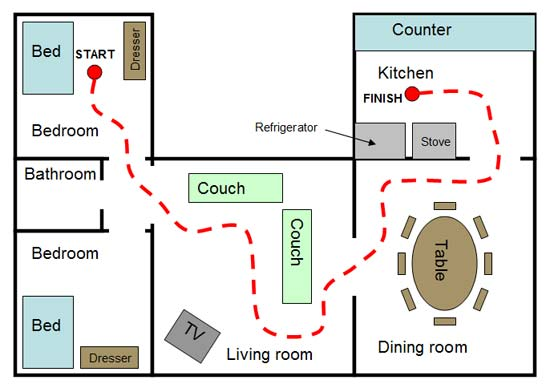
\includegraphics[width=0.85\textwidth, height=0.70\textheight]{figures/planning01.jpg}
%%%prolog/scale=0.47
%\label{fig_nos_estados}
\caption{\textit{A fome no meio da noite!}}
\end{figure}

%\framebreak

\end{frame}


\begin{frame}[fragile]
\frametitle{Exemplos do que é planejamento ...}

\begin{figure}[!htb]
\centering
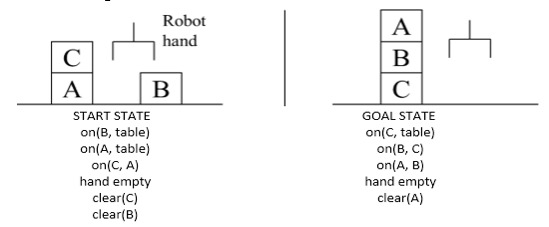
\includegraphics[width=0.850\textwidth, height=0.650\textheight]{figures/mundo_dos_blocos01.jpg}
%%%prolog/scale=0.47
%\label{fig_nos_estados}
\caption{O \textit{mundo dos blocos}}
\end{figure}

%\framebreak

\end{frame}


\begin{frame}[fragile]
\frametitle{Espaço de Estados}

\begin{figure}[!htb]
\centering
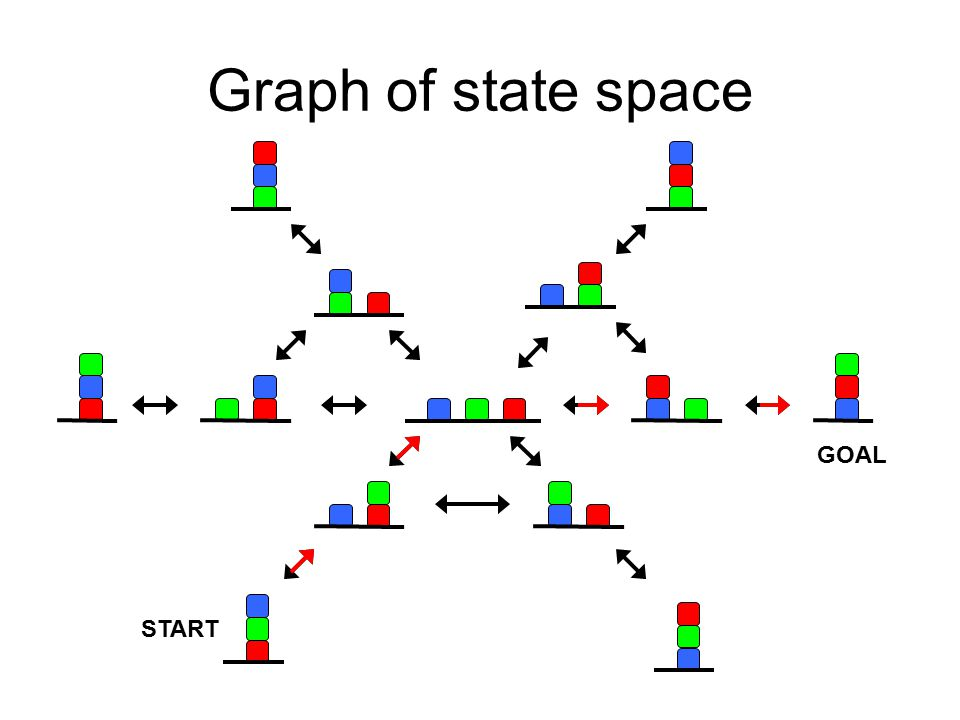
\includegraphics[width=0.7\textwidth, height=0.70\textheight]{figures/mundo_dos_blocos02.jpg}
%%%prolog/scale=0.47
%\label{fig_nos_estados}
\caption{O espaço de estados do \textit{mundo dos blocos} $\times$ ações}
\end{figure}

%\framebreak

\end{frame}



\begin{frame}[fragile, allowframebreaks=0.9]
\frametitle{Elementos de um  Planejador -- Vocabulário}

%%%%\textcolor{red}{PAREI AQUI}

\begin{itemize}
 \item \underline{Plano}: uma sequência ordenada de ações, 
 criada incrementalmente a partir do estado inicial\\
Ex. posições das peças de um jogo\\
$$S_1 < S_2 < ... < S_n$$
 
  \item \underline{Ambiente}: onde um programa--agente vai receber entradas em um determinado
  estado e atuar com uma ação apropriada

  \item  \underline{Estados}:   descrição completa de possíveis estados atingíveis\\
  Problema: quanto aos estados não-previstos, inacessíveis?

  \item  \underline{Estado inicial}: um estado particular onde nosso programa--agente
  inicia a sua busca
  
  \item \underline{Objetivos}: estados desejados que o programa--agente precisa alcançar,
  isto é, um dos \textit{estados finais} desejados

  \item  \underline{Percepções}: cheiro, brisa, luz, choque,
  som, posições ou coordenadas, vizinhanças, etc

  \item \underline{Ações}: provocam modificações entre os estados corrente e sucessor\\
  Exemplos: avançar para próxima célula, girar 90 graus à direita ou à esquerda
pegar um objeto, atirar na direção do alvo, etc
 
 \item \underline{Operadores}: vocabulário ou repertório de atuações atômicas do que o agente pode fazer.\\
 Exemplos: $pegar(X)$, $mover\_de(X,Y)$, $levantar(X)$, $livre(X)$, etc
 
 \item Uma eventual confusão: \textcolor{magenta}{\textbf{uma ação é um conjunto de um ou mais operadores}},
 e ainda, \textcolor{magenta}{\textbf{a ação é condicional}}. 
 A ação só é disparada se as condições de pré-requisitos forem 
 satisfeitas.
 
 \item \underline{Heurística}: alguma função que  indica o progresso sobre os estados
 não visitados e sua convergência para uma finalização do plano
 
 
\end{itemize}

\end{frame}



\begin{frame}[fragile, allowframebreaks=0.9]
  \frametitle{O Problema Exemplo}

\begin{figure}[!htb]
\centering
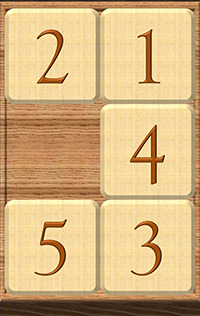
\includegraphics[width=.3\textwidth, height=0.40\textheight]{figures/puzzle_2x3_01.jpg}
%%%prolog/scale=0.47
%\label{fig_nos_estados}
\caption{Um quebra-cabeça ($2\times 3$ ou $3\times 2$) \textit{simplificado} do conhecido $3\times 3$}
\end{figure}


\framebreak
\begin{figure}[!htb]
\centering
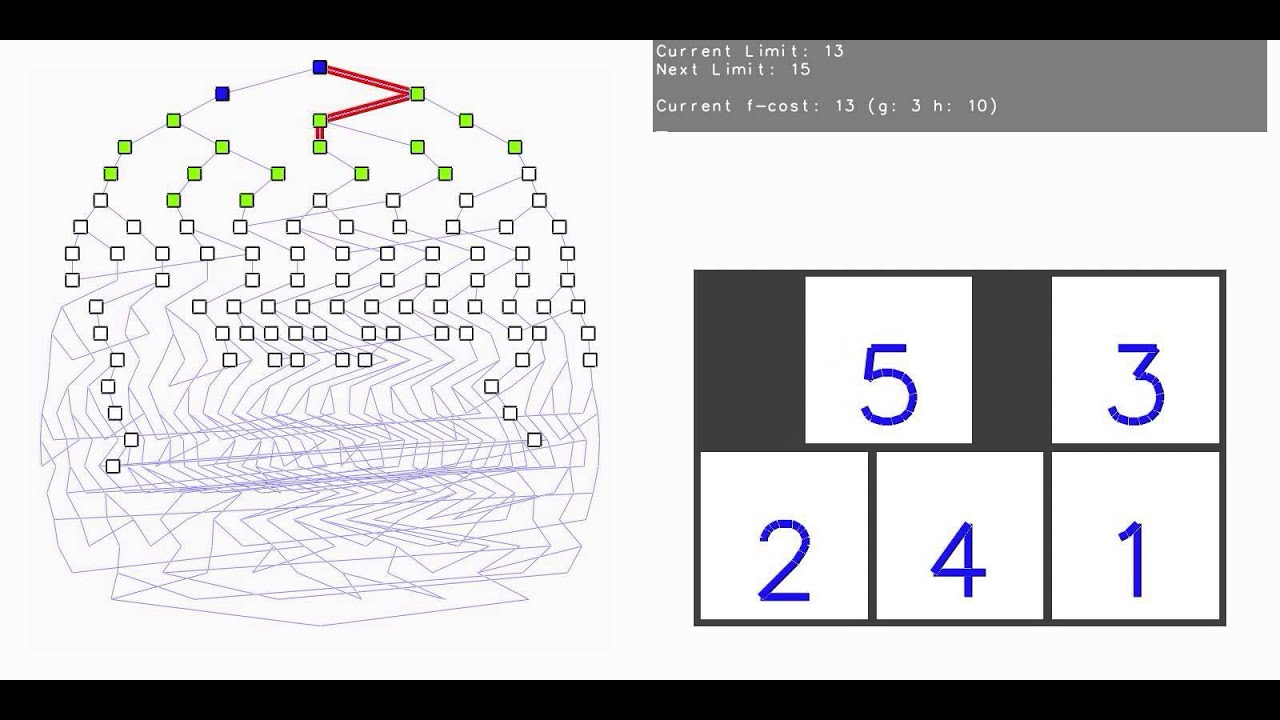
\includegraphics[width=.75\textwidth, height=0.65\textheight]{figures/puzzle_2x3_02.jpg}
%%%prolog/scale=0.47
%\label{fig_nos_estados}
\caption{Sim, \textit{simplificado} mas não muito!}
\end{figure}

\end{frame}

\begin{frame}[fragile, allowframebreaks=0.9]
 \frametitle{Partes do  código comentado}


\begin{footnotesize}
\begin{verbatim}
/*
A  B  C 
D  E  F
*/

%%%%%%%%%
%   1 5 %
% 4 3 2 %
%%%%%%%%%

import datetime.
import planner.
\end{verbatim}
\end{footnotesize}

\begin{center}
\textbf{\textcolor{red}{Atenção quanto a modelagem do problema, as 3 primeiras posicões da lista
correspondem a linha superior (A .. C), e as 3 últimas, a linha inferior (D .. F).}
}
\end{center}

\framebreak

\begin{footnotesize}
\begin{verbatim}
index(-)
estado_inicial( [0,1,5,4,3,2]  ).
%%%%%%%%%%%%%==> A,B,C,D,E,F

%% funcao final do planner
final( [1,2,3,4,5,0] ) => true .
%%%%==> A,B,C,D,E,F
%% pode ter uma condicional de parada

\end{verbatim}

\end{footnotesize}
\framebreak

\begin{footnotesize}
\begin{verbatim}
% Up <-> Down
/* Descrevendo as possiveis acoes para o planner */
action([A,B,C, D,E,F], S1, Acao, Custo_Acao ) ?=>
    Custo_Acao = 1,
    ( A == 0 ),  %% conj. condicoes
    S1 = [D,B,C, 0,E,F], 
    Acao = ($up(D),S1). %%a acao + estado modificado

action([A,B,C, D,E,F], S1, Acao, Custo_Acao ) ?=>
    Custo_Acao = 1,
    (A == 0 ),  %% conj. condicoes
    S1 = [0,B,C, A,E,F],
    Acao = ($dow(A),S1). %%a acao + estado modificado
.........................................................
\end{verbatim}
\end{footnotesize}

\framebreak


\begin{footnotesize}
\begin{verbatim}
% Left <-> Right
action([A,B,C, D,E,F], S1, Acao, Custo_Acao ) ?=>
    Custo_Acao = 1,
    (A == 0),  %% conj. condicoes
    S1 = [B,0,C, D,E,F],
    Acao = ($left(B), S1). %%a acao + estado modificado
    
action([A,B,C, D,E,F], S1, Acao, Custo_Acao ) ?=>
    Custo_Acao = 1,
    (B == 0),  %% conj. condicoes
    S1 = [0,A,C, D,E,F],
    Acao = ($right(A), S1). %%a acao + estado modificado
.........................................................
\end{verbatim}

\end{footnotesize}
\framebreak

\begin{footnotesize}
\begin{verbatim}
main  ?=>  
    estado_inicial( Q ),
    best_plan_unbounded( Q , Sol_Acoes), 
    println(sol = Sol_Acoes),
        
    printf("\n Estado Inicial: "),
    w_Quadro( Q ), 
    w_L_Estado( Sol_Acoes ), 
    Total := length(Sol_Acoes) ,
    Num_Movts := (Total -1) ,
    printf("\n Inicial  (estado): %w ", Q),
    printf("\n Total de acoes: %d", Total), 
    printf(" \n =========================================\n ")
    %%% fail ou false: descomente para multiplas solucoes
    .
 main => printf("\n Para uma solução .... !!!!" ) .
\end{verbatim}

\end{footnotesize}

\end{frame}



\begin{frame}[fragile]
 \frametitle{O código}

\begin{itemize}
  \item Acompanhar as explicações do código de:\\
\url{https://github.com/claudiosa/CCS/blob/master/picat/puzzle_2x3_planner.pi}

  \item Confira a execuç\~ao
\end{itemize}
\end{frame}


\begin{frame}[fragile, allowframebreaks=0.9]
 \frametitle{Parte da Saída}

\begin{footnotesize}
\begin{verbatim}
[ccs@gerzat picat]$ picat puzzle_2x3_planner.pi 
sol = [(left(1),[1,0,5,4,3,2]),(left(5),[1,5,0,4,3,2]),
(up(2),[1,5,2,4,3,0]),(right(3),[1,5,2,4,0,3]),(dow(5),[1,0,2,4,5,3]),
(left(2),[1,2,0,4,5,3]),(up(3),[1,2,3,4,5,0])]

 Estado Inicial: 
 0 1 5
 4 3 2

Acao: left(1)
 1 0 5
 4 3 2

Acao: left(5)
 1 5 0
 4 3 2
\end{verbatim}
\end{footnotesize}

\framebreak
\begin{footnotesize}
\begin{verbatim}
.................................
Acao: left(2)
 1 2 0
 4 5 3

Acao: up(3)
 1 2 3
 4 5 0

 Inicial  (estado): [0,1,5,4,3,2] 
 Total de acoes: 7 
 =========================================
\end{verbatim}
\end{footnotesize}

\end{frame}



\begin{frame}[fragile]
 \frametitle{O módulo do \textit{planner} do Picat}

\begin{itemize}
  \item O que efetivamente voce precisa saber
  
  \pause
  \item Importar um módulo \\
   \textbf{\texttt{import planner.}}

   \pause
   \item O predicado: \textit{final}\\
    \textbf{\texttt{final(S,Plan,Cost) => Plan=[], Cost=0, final(S).}}
   
    \pause
    \item O predicado \textit{action}\\
    \textbf{\texttt{action(S,NextS,Action,ActionCost)}}

\end{itemize}
\end{frame}


\begin{frame}[fragile]
 \frametitle{O módulo do \textit{planner} do Picat}

\begin{itemize}

 \item A \textcolor{magenta}{\textbf{eficiência}} do planner do Picat se dá devido a sua combinação
       de técnicas: \textcolor{magenta}{busca em profundidade} (e variações) e \textcolor{magenta}{Programação
       Dinâmica (PD)} (uso do \textit{tabling})


  \pause 
  \item O núcleo de busca dos planejadores  disponíveis no Picat são de 2 tipos:
  \begin{enumerate}
    \item Usam um busca em profundidade com limites (\textit{Depth-Bounded Search})
    \item Usam um busca em profundidade ilimitada de recursos (\textit{Depth-Unbounded Search}) 
  \end{enumerate}
  
  \item Contudo, estes 2 tipos apresentam muitas variações e opções:\\
  \pause
  Sem escapatória $\Rightarrow $ consultar o manual do Picat (\textit{User Guide to Picat})
  
  \item No exemplo aqui apresentado: 
  \texttt{best\_plan\_unbounded(S,Plan)}   
\end{itemize}
\end{frame}




\begin{frame}[fragile]
\frametitle{Reflexões}


\begin{itemize}
  \item Planejamento resolve uma classe ampla de problemas\\
   Havendo necessidade de
    \textcolor{magenta}{\textbf{descobrir sequências ações}} $\Leftrightarrow$ \textcolor{violet}{Planejamento}

  \pause
  \item Em geral, estes problemas são importantes na indústria

  \pause
  \item Os modelos escritos em PDDL (\textit{Planning Domain Definition Language})
  facilmente portáveis para Picat
    \pause
  \item Sob um uso mais restrito, um modelo em PDDL é executado diretamente em Picat
    
  \pause
  \item Na próxima seção uma outra técnica de resolver problemas: \textbf{\underline{PR}}
\end{itemize}

\end{frame}



       
\section{Programação por Restrições}

\begin{frame}[fragile]
%[fragile, allowframebreaks=0.9]

    \frametitle{Programação por Restrições (PR) -- I}

   \begin{block}{}
     \begin{itemize}
     
      \item A Programação por Restrições (PR) é conhecida por \textit{Constraint Programming} ou simplesmente \textbf{CP}

      \pause
      \item Uma poderosa teoria (e técnica)  que  contorna a complexidade de certos problemas
      exponenciais
      
       
      \pause
      \item A PR encontrava-se inicialmente dentro da IA e PO, mas como várias outras, tornaram-se
      fortes e autônomas. Atualmente uma área de pesquisa bem forte em alguns países.
      
     
    \end{itemize}
    
    \end{block}
    
\end{frame}




\begin{frame}[fragile]
%[fragile, allowframebreaks=0.9]

    \frametitle{Programação por Restrições (PR) -- II}

   \begin{block}{}
     \begin{itemize}

      \item Aproximadamente o algoritmo da PR é dado:
       \pause       
          \begin{enumerate}

            \item Avaliar algebricamente  os domínios das variáveis com suas restrições

            \item Intercala iterativamente a \textsf{propagação de restrições} com 
                  um \textsf{algoritmo de busca}

            \item A cada variável instanciada, o processo é repetido sobre as demais variáveis, reduzindo progressivamente o espaço de busca

            \item Volte ao passo inicial até que os domínios permaneçam estáticos
            e que as variáveis apresentem instâncias consistentes
              
          \end{enumerate}
       
        \pause
       \item Este núcleo é uma busca por constantes otimizações

        \pause
       \item Uma das virtudes da PR: a legibilidade e clareza de suas soluções
       
    \end{itemize}
    
    \end{block}
    
\end{frame}


\begin{frame}[fragile]
%[fragile, allowframebreaks=0.9]
\frametitle{Programação por Restrições (PR) -- III}

   \begin{block}{}
     \begin{itemize}
    \item Problemas combinatoriais com domínio nos inteiros são bons candidatos a serem
       resolvidos por PR
       \pause
       \item Quando temos problemas que precisamos conhecer \textbf{todas} as respostas, 
    não apenas a melhor resposta
    
      \pause
      \item Quando necessitamos de respostas \textit{precisas} e não apenas as aproximadas.
       Há um custo  computacional a ser pago aqui!
        
        \pause
        \item



    \end{itemize}
    \end{block}
    
\end{frame}



\begin{frame}[fragile]
%[fragile, allowframebreaks=0.9]

\frametitle{Metodologia da  Construção de Modelos}

\begin{figure}[ht!]
\begin{center}

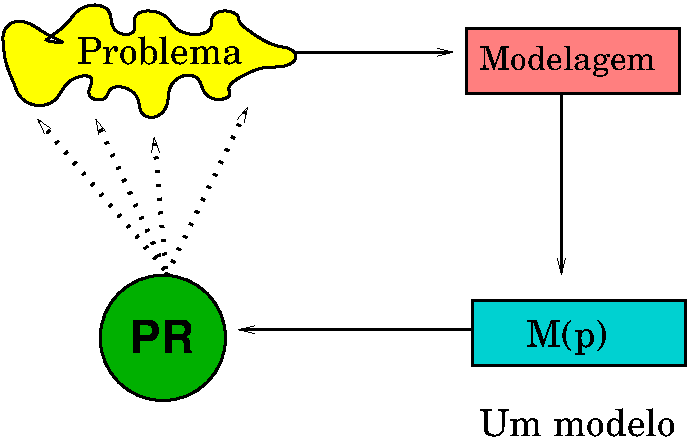
\includegraphics[width=0.70\textwidth, height=0.60\textheight]{figures/problema_modelagem.pdf}

\end{center}
\end{figure}


    
\end{frame}


\begin{frame}[fragile]
%[fragile, allowframebreaks=0.9]

\frametitle{Fluxo de Cálculo da PR}

\begin{figure}[!htb]
\centering
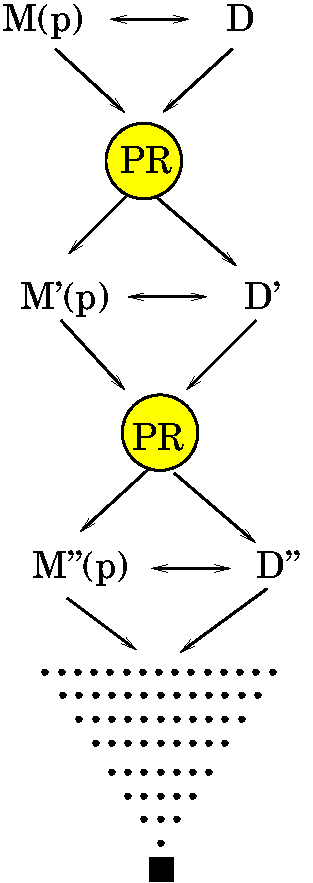
\includegraphics[width=0.30\textwidth, height=0.75\textheight]{figures/dinamica_pr.pdf}
\end{figure}
   
\end{frame}



\begin{frame}[fragile]
%[fragile, allowframebreaks=0.9]

\frametitle{Onde o objetivo da PR é:}

\begin{figure}[!htb]
\begin{center}
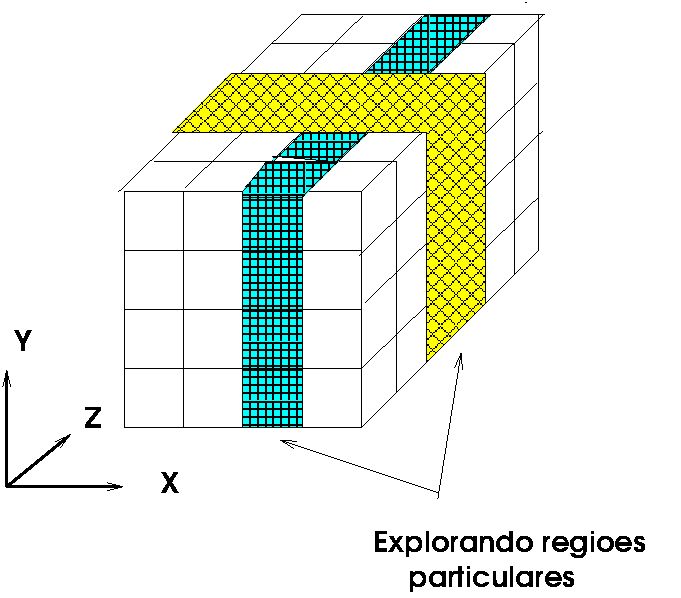
\includegraphics[width=0.70\textwidth, height=0.60\textheight]{figures/reducao_PR_01.pdf}
\caption{Realizar buscas com regiões reduzidas -- promissoras (regiões factíveis de soluções)}
\end{center}
\end{figure}
    
\end{frame}




\begin{frame}[fragile]
%[fragile, allowframebreaks=0.9]

\frametitle{Redução Iterativa em Sub-problemas}

\begin{figure}[!htb]

\begin{center}
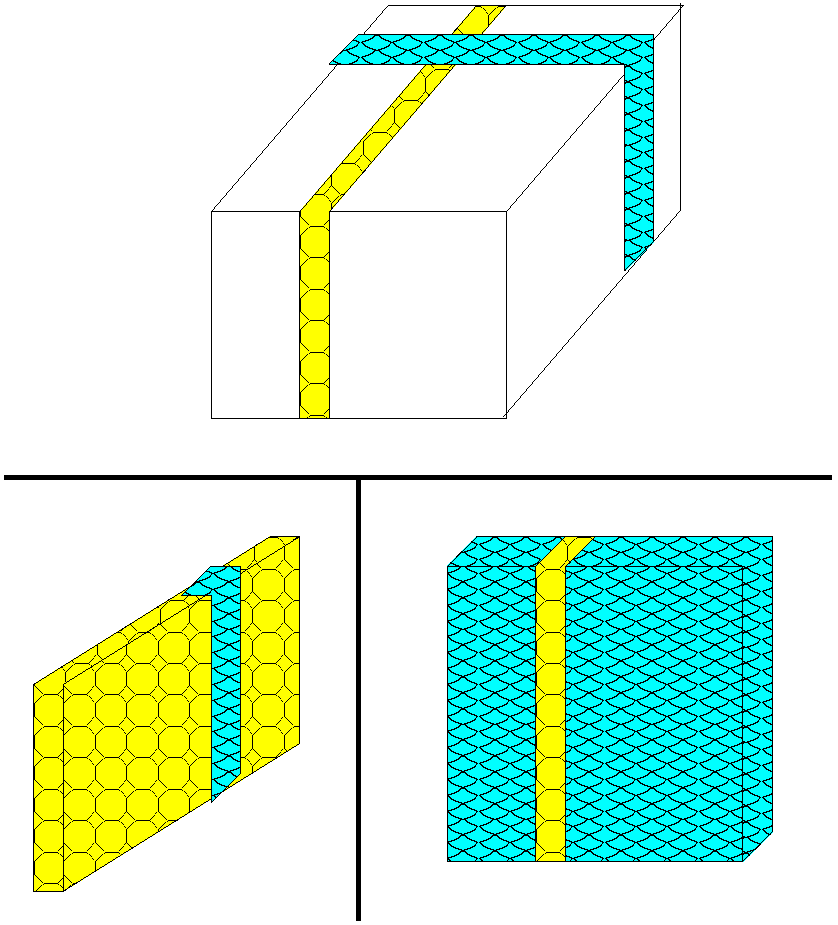
\includegraphics[width=0.70\textwidth, height=0.60\textheight]{figures/reducao_PR_02.pdf}
\caption{Redução de um CP em outros sub-problemas CPs equivalentes}
\end{center}
\end{figure}

    
\end{frame}



\begin{frame}[fragile]
%[fragile, allowframebreaks=0.9]
\frametitle{Conceitos}

\begin{block}{A PR tem os seguintes elementos:}
\pause
\begin{itemize}
  \item Um conjunto de \textbf{variáveis}: $X_1$, $X_2$, $X_3$, ..., $X_n$ 

  \pause
    \item Um conjunto de \textbf{domínios} dessas variáveis: $D_{X_1}$, $D_{X_2}$, $D_{X_3}$, ..., $D_{X_n}$

    \pause
      \item Finalmente, as \textbf{restrições}, que são relações n-árias entre estas variáveis
      
       \pause
      \item Exemplo: $D_{X_1} = D_{X_2}= \{3,4\}$ e $X_1 \neq X_2$
      
\end{itemize}

\end{block}
    
\end{frame}


\begin{frame}[fragile]
%[fragile, allowframebreaks=0.9]
\frametitle{PR e Picat}

\begin{block}{}

\begin{itemize}
    \item Para o exemplo anterior um  código em Picat é dado por:
      \pause
    \begin{itemize}
        \item \texttt{[X1, X2] :: 3..4}
        \item \texttt{X1 \#!= X2} 
     \end{itemize}  
      
      \pause
     \item Em resumo, as relações da PR tem o símbolo `{\#}' 

  \pause
  \item Para tornar toda esta sintaxe da PR disponível, Picat tem um módulo para suporte da PR: \texttt{import cp}
    
\end{itemize}

\end{block}
    
\end{frame}


\begin{frame}[fragile] 

\frametitle{Exemplo -- 01 -- Soma de Números Primos}

\begin{itemize}
  \item Dado um número par qualquer, encontre  dois de números primos, $N_1$ e $N_2$,
diferentes entre si, que somados deêm este número 
par.

\pause
\item Exemplo:\\
Seja o PAR = 18\\
Uma soluç~ao:\\
$N_1 = 7$  e $N_2 = 11$\\
pois\\
$N_1 + N_2 = 18$
\end{itemize}

\end{frame}
%%%%%%%%%%%%%%%%%
\begin{frame}[fragile] 

\frametitle{Modelagem do Problema}

\begin{itemize}
  \item  $N_1$ e $N_2$ assumem valores no domínio dos números primos. \\
  Logo, é importante ter os números primos prontos!

  \pause
   \item A soma destes números é o par fornecido como entrada, $N_{PAR}$:\\
         $N_1 + N_2 = N_{PAR}$

  \pause
  \item  $N_1$ e $N_2$  são diferentes entre si\\
   $N_1 \neq N_2$

  \pause
  \item Como são inteiros: $N_1 < N_{PAR}$ e $N_2 < N_{PAR}$ \\
  Sim, é óbvio, mas isto faz uma redução significativa de domínio!

\end{itemize}

\end{frame}


%%%%%%%%%%%%%%%%%%%%%%%%%%
\begin{frame}[fragile]
 \frametitle{Código Completo}

\begin{itemize}
  \item Acompanhar as explicações do código de:\\
\url{https://github.com/claudiosa/CCS/blob/master/picat/soma_N1_N2_primos_CP.pi}

  \item Confira a execução e testes
\end{itemize}
\end{frame}


%%%%%%%%%%%%%%%%%%%%%%%%%%
\begin{frame}[fragile] 

\frametitle{Código em Partes}

\begin{small}
\begin{verbatim}
modelo => 
    PAR = 382,
    Variaveis = [N1,N2],
    % Gerando um domino soh de primos
    % L_dom = [I : I in 1..1000, eh_primo(I) == true],   %OU
    L_dom = [I : I in 1..1000, prime(I)],
    Variaveis :: L_dom,
\end{verbatim}
\end{small}
   
   Uma ótima estratégia: sair com um domínio de números candidatos!
    
\end{frame}
%%%%%%%%%%%%%%%%%
\begin{frame}[fragile] 

\frametitle{Código em Partes}

\begin{small}
\begin{verbatim}
    % RESTRICOES
    N1 #!= N2,
    N1 #< PAR,  
    N2 #< PAR,
    N1 + N2 #= PAR,
  
	% A BUSCA
	solve([ff], Variaveis),
  % UMA SAIDA
	printf("\n  N1: %d\t N2: %d", N1,N2),
	printf("\n.....................................")
	.
\end{verbatim}
\end{small}
    
\end{frame}
%%%%%%%%%%%%%%%%%
\begin{frame}[fragile] 

\frametitle{Código em Partes}

\begin{small}
\begin{verbatim}
import cp.

% main => modelo	.
% main ?=> modelo, fail.	
% main =>  true.	

main =>
    L = findall(_, $modelo),
    writef("\n Total de solucoes:  %d \n", length(L)) .

\end{verbatim}
\end{small}
    
\end{frame}


\begin{frame}[fragile]
%[fragile, allowframebreaks=0.9]

\frametitle{Saída -- I}

\begin{small}
\begin{verbatim}
Picat> cl('soma_N1_N2_primos_CP').
Compiling:: soma_N1_N2_primos_CP.pi
** Warning  : redefine_preimported_symbol(math): prime / 1
soma_N1_N2_primos_CP.pi compiled in 7 milliseconds
loading...

yes

Picat> main.                      

  N1: 3	 N2: 379
.....................................
  N1: 23	 N2: 359
.....................................
  N1: 29	 N2: 353
.....................................
\end{verbatim}
    
\end{small}
\end{frame}


\begin{frame}[fragile]
%[fragile, allowframebreaks=0.9]

\frametitle{Saída -- II}

\begin{small}
\begin{verbatim}
 .....................................
  N1: 353	 N2: 29
.....................................
  N1: 359	 N2: 23
.....................................
  N1: 379	 N2: 3
.....................................
 Total de solucoes:  18 

yes

Picat> 
\end{verbatim}
    
\end{small}
\end{frame}
%%%%%%%%%%%%%%%%%%%%%%%%%%%%%%%%%%%%%%%%%%%%%%%%%%%%%%%%%%%%%%%%%%%%
\begin{frame}[fragile] 

\frametitle{Exemplo -- 02 -- Escala de Consultórios}

\begin{itemize}
\item Seja um Posto Atendimento Médico, um PA, com 4 consultórios e 7 especialidades
  médicas

\pause
\item O problema é distribuir estes médicos nestes 4 consultórios
tal que alguns requisitos sejam atendidos (restrições  satisfeitas)

\pause
\item A abordagem aqui é ingênua e sem muitos critérios
\end{itemize}

\end{frame}
\begin{frame}[fragile] 

\frametitle{Modelagem do Problema}

\begin{itemize}
  \item  Vamos usar uma matriz bi-dimensional para 
  representar o problema. Linhas $\leftrightarrow$ consultórios (1 a 4), e 
  as colunas $\leftrightarrow$ dias da semana (1 a 5)

  \pause
  \item Esta matriz será preenchida com valores/códigos de 1 a 7, de acordo com a especialidade médica.
  
  \pause
  \item Assim o domínio da matriz \texttt{Quadro} ($4 \times 5$) será
  preenchida com um destes códigos.
   
  \pause
  \item Vamos utilizar restrições globais: \texttt{member} e \texttt{all\_different}

  \pause
  \item As restrições globais se aplicam sobre um conjunto de variáveis.


\end{itemize}

\end{frame}

%%%%%%%%%%%%%%%%%%%%%%%%%%%%%%%%%%%%%%%%%%%%%
\begin{frame}[fragile] 

\frametitle{Modelagem -- Comentários}

\begin{itemize}
  \item A fase de busca e propagação do comando 	\texttt{solve(Critérios, Variáveis)}, 
  há dezenas de combinações possíveis: consultar o guia do usuário
  
  \pause
  \item Tem-se os predicados extras ... são muitos, todos os da CP

  \pause
  \item Finalmente, exemplos sofisticados-- de PR com PICAT:\\
  \url{http://www.hakank.org/picat/} -- \textit{\textbf{My Picat page}} --
  por Hakan Kjellerstrand 

\end{itemize}

\end{frame}

%%%%%%%%%%%%%%%%%%%%%%%%%%
\begin{frame}[fragile]
 \frametitle{Código Completo}

\begin{itemize}
  \item Acompanhar as explicações do código de:\\
\url{https://github.com/claudiosa/CCS/blob/master/picat/horario_medico_CP.pi}

  \item Confira a execução e testes
\end{itemize}
\end{frame}


%%%%%%%%%%%%%%%%%%%%%%%%%%%%%%%%%%%%%%%%%%%%%%%%%%%%
\begin{frame}[fragile] 

\frametitle{Código em Partes}

\begin{small}
\begin{verbatim}
modelo => 
    Dias = 5, % segunda= 1, ...., sexta-feira = 5
    Consultorio = 4,
    L_dom = [ oftalmo, otorrino, pediatra,  gineco, 
%                1        2          3         4
              cardio, dermato, clin_geral ],
%                5       6        7
   Quadro = new_array(Consultorio, Dias ), %% Lin x Col
   Quadro :: 1 .. L_dom.len , %% operador len . "eh colado"
...
\end{verbatim}
\end{small}
   
    
\end{frame}
%%%%%%%%%%%%%%%%%%%%%%%%%%%%%%%%%%%%%%%%%%%%%%%%%%%%
\begin{frame}[fragile] 

\frametitle{Código em Partes}

\begin{small}
\begin{verbatim}
    %% O medico 2 NUNCA trabalha no consultorio 1
    foreach ( J in 1 .. Dias ) 
        Quadro[1,J] #!= 2
    end,
    
    %% O medico 5 NUNCA trabalha no consultorio 4
    foreach ( J in 1 .. Dias ) 
        Quadro[4,J] #!= 5
    end,
...
\end{verbatim}
\end{small}
    
\end{frame}
%%%%%%%%%%%%%%%%%%%%%%%%%%%%%%%%%%%%%%%%%%%%%%%%%%%%
\begin{frame}[fragile] 

\frametitle{Código em Partes}

\begin{small}
\begin{verbatim}

  %% O Clin Geral deve vir o maior numero de dias ... 
  %% Esta restricao eh matematicamente é HARD
   foreach ( I in 1 .. Consultorio )
     member(7,[Quadro[I,J] : J in 1..Dias]) 
   end,  
  
  %% Ninguém trabalha no mesmo consultorio em dias seguidos
  foreach ( J in 1 .. Dias )
      all_different( [Quadro[I,J] : I in 1..Consultorio] )
  end,  
 
  %% Ninguém trabalha no mesmo dia em mais de um consultorio
   foreach ( I in 1 .. Consultorio )
      all_different( [Quadro[I,J] : J in 1..Dias] )
   end,  
...  
\end{verbatim}
\end{small}
    
\end{frame}
%%%%%%%%%%%%%%%%%%%%%%%%%%%%%%%%%%%%%%%%%%%%%%%%%%%%
\begin{frame}[fragile] 

\frametitle{Código em Partes}

\begin{small}
\begin{verbatim}
	% A BUSCA
	solve([ff], Quadro),
  % UMA SAIDA
	
   printf("\n Uma escolha:"),
   print_matrix( Quadro ),
   print_matrix_NAMES( Quadro , L_dom ),
	 printf(".............................\n") .
\end{verbatim}
\end{small}
    
\end{frame}
%%%%%%%%%%%%%%%%%%%%%%%%%%%%%%%%%%%%%%%%%%%%%%%%%%%%
\begin{frame}[fragile] 

\frametitle{Código em Partes}

\begin{small}
\begin{verbatim}
print_matrix_NAMES( M, Lista ) =>
 L = M.length,
 C = M[1].length,
  nl,
   foreach(I in 1  .. L)
     foreach(J in 1  ..  C)
      printf(":%w \t" , print_n_lista( M[I,J], Lista) )
     % printf("(%d,%d): %w " , I, J, M[I,J] ) -- FINE
     end,
     nl
   end.
%%%%%%%%%%%%%%%%%%%%%%%%%%%%%%%%%%%%%%%%%%%%%%%%%%%%%%%%%%%%%%%%%%
print_n_lista( _, [] ) =  [].
print_n_lista( 1, [A|_] ) = A.
print_n_lista( N, [_|B] ) = print_n_lista( (N-1), B ) .
%%%%%%%%%%%%%%%%%%%%%%%%%%%%%%%%%%%%%%%%%%%%%%%%%%%%%%%%%%%%%%%%%%
\end{verbatim}
\end{small}
    
\end{frame}
%%%%%%%%%%%%%%%%%%%%%%%%%%%%%%%%%%%%%%%%%%%%%%%%%%%%


\begin{frame}[fragile]
%[fragile, allowframebreaks=0.9]

\frametitle{Saída - I}

\begin{small}
\begin{verbatim}
Picat> cl('horario_medico_CP.pi').
Compiling:: horario_medico_CP.pi
horario_medico_CP.pi compiled in 10 milliseconds
loading...

yes

Picat> main                       

 Uma escolha:
7 1 3 4 5 
4 7 2 3 1 
1 3 7 5 2 
3 2 1 7 4 
\end{verbatim}
  
\end{small}
\end{frame}

%%%%%%%%%%%%%%%%%%%%%%%%%%%%%%%%%%%%%%%%%%%%%%%%%%%%

\begin{frame}[fragile]
%[fragile, allowframebreaks=0.9]

\frametitle{Saída - II}

\begin{small}
\begin{verbatim}
:clin_geral 	:oftalmo 	:pediatra 	:gineco 	:cardio 	
:gineco 	:clin_geral 	:otorrino 	:pediatra 	:oftalmo 	
:oftalmo 	:pediatra 	:clin_geral 	:cardio 	:otorrino 	
:pediatra 	:otorrino 	:oftalmo 	:clin_geral 	:gineco 	
....................................
yes
\end{verbatim}
  
\end{small}
\end{frame}

\begin{frame}[fragile]
%[fragile, allowframebreaks=0.9]

\frametitle{Saída - III}

\begin{small}
\begin{verbatim}

$ time(picat horario_medico_CP.pi )

 Uma escolha:
7 1 3 4 5 
4 7 2 3 1 
1 3 7 5 2 
3 2 1 7 4 

:clin_geral 	:oftalmo 	:pediatra 	:gineco 	:cardio 	
:gineco 	:clin_geral 	:otorrino 	:pediatra 	:oftalmo 	
:oftalmo 	:pediatra 	:clin_geral 	:cardio 	:otorrino 	
:pediatra 	:otorrino 	:oftalmo 	:clin_geral 	:gineco 	
....................................
real	0m0,023s
user	0m0,007s
sys	0m0,013s
[ccs@gerzat picat]$ 
\end{verbatim}
  
\end{small}
\end{frame}

%%%%%%%%%%%%%%%%%%%%%%%%%%%%%%%%%%%%%%%%%%%%%%%%%%%%

\begin{frame}[fragile]
\frametitle{Reflexões}


\begin{itemize}
  \item Há outros métodos para se resolver estes problemas.\\
  Exemplo: Programação Linear, Buscas Heurísticas, etc

  \pause  
  \item As restrições globais se aplicam sobre um conjunto de variáveis
  e há muitas outras importantes disponíveis no Picat

  \pause
  \item A área é extensa, contudo, Picat adere há todos requisitos da PR

    \pause
  \item Resumo da PR: segue por uma notação/manipulação algébrica restrita,
        simplificar e bissecionar as restrições, instanciar variáveis, 
        verificar inconsistências,
        avançar sobre as demais variáveis, até que todas 
        estejam instanciadas.
  
\end{itemize}

\end{frame}
 % cap  finalizar aqui

\section{Conclusões}
%%%%%%%%%%%%%%%%%%%%%%%%%%
\begin{frame}[fragile]
\frametitle{Conclusões}
\begin{minipage}{0.47\textwidth}
    \begin{itemize}
        \item O que foi visto
        \item O que tem a ser feito
        \item Oportunidades
    \end{itemize}
\end{minipage}
\begin{minipage}{0.5\textwidth}
\begin{figure}[ht!]
\begin{center}
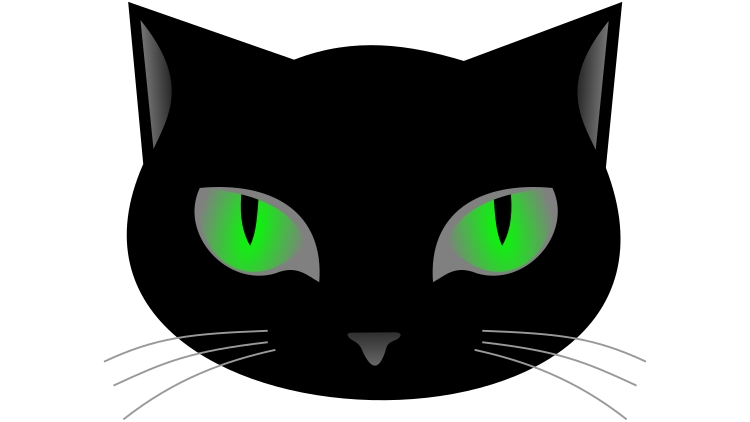
\includegraphics[width=1.2\textwidth, height=0.40\textheight]{figures/logo_picat_alex.jpg}
\end{center}
\end{figure}
\end{minipage}
\end{frame}
%%%%%%%%%%%%%%%%%%%%%%%%%%
\begin{frame}[fragile]

    \frametitle{Conclusões}

    \begin{itemize}
      \item Picat é jovem (nascida em 2013); 
      \pause
      \item Uma evolução ao Prolog após seus mais de 40 anos de existência e sucesso!
      \pause
      \item Sua sintaxe é moderna e intuitiva;
      \pause
      \item Código aberto, multi-plataforma, e repleta de possibilidades;
      \pause
      \item Uso para fins diversos;
      \pause
      \item Muitas bibliotecas específicas prontas: CP, SAT, Planner, etc;
      \pause
      \item A sintaxe de PR exige um pouco mais do programador
      \pause
      \item Dúvidas: o guia do usuário, livro do Hakan e o Fórum de discussão do Picat

    \end{itemize}
\end{frame}


%%%%%%%%%%%%%%%%%%%%%%%%%%

\subsection{Faltando}
\begin{frame}[fragile]

    \frametitle{O que ficou faltando:}

    \begin{itemize}
      \item Uso do \texttt{debug} e \texttt{trace} (cansativo -- uma oportunidade)
      \pause
      \item Explorar uso dos solvers de PO (fácil)

      \pause
      \item Explorar a criação e  uso de módulos  (mais fácil ainda)

      \pause
      \item Inscreva-se no fórum e consulte o Guia do Usuário (tudo em inglês)


    \end{itemize}
\end{frame}


\subsection{Agradecimentos}
\begin{frame}[fragile]

    \frametitle{Agradecimentos}

    \begin{itemize}
      \item Muito obrigado a voce!
      \pause
      \item Algumas pessoas que deram opiniões e me incentivaram a 
            fazer este material
  
      \pause
      \item Claudio Cesar de Sá
     \item Contacto: \url{claudio.sa@udesc.br} e\\
           \url{claudio@colmeia.udesc.br}

    \end{itemize}
\end{frame}

\end{document}
